\documentclass[11pt]{article}
\usepackage[a4paper,margin=21mm]{geometry}
\usepackage{fontspec}
\setmainfont{Latin Modern Roman}
\newfontfamily\CJKfont{Noto Serif CJK SC}
\XeTeXlinebreaklocale "zh"
\XeTeXlinebreakskip=0pt plus 1pt
\usepackage{amsmath,amssymb,amsthm,amscd,graphicx,color}
\usepackage{xurl}
\usepackage[unicode,hidelinks]{hyperref}
\allowdisplaybreaks
\setlength\emergencystretch{3em}
\numberwithin{equation}{section}

\usepackage{amstext}
\usepackage{amscd}
\usepackage{enumerate}
\usepackage{mathrsfs}
\usepackage{mathtools}

\usepackage{tikz}
\usepackage{tikz-cd}
\usetikzlibrary{arrows}
\usetikzlibrary{decorations.markings}
\usetikzlibrary{patterns,decorations.pathreplacing}

\numberwithin{equation}{section}
\numberwithin{figure}{section}
\numberwithin{table}{section}

\newtheorem{Theorem}{Theorem}[section]
\newtheorem*{Theorem*}{Theorem}
\newtheorem{Corollary}[Theorem]{Corollary}
\newtheorem{Lemma}[Theorem]{Lemma}
\newtheorem{Proposition}[Theorem]{Proposition}
 { \theoremstyle{definition}
\newtheorem{Definition}[Theorem]{Definition}
\newtheorem{Note}[Theorem]{Note}
\newtheorem{Example}[Theorem]{Example}
\newtheorem{Remark}[Theorem]{Remark}
\newtheorem{observation}[Theorem]{Observation}
\newtheorem{operation}[Theorem]{Operation}
\newtheorem{setting}[Theorem]{Setting}}

\newcommand{\ZZ}{\mathbb{Z}}
\newcommand{\QQ}{\mathbb{Q}}
\newcommand{\RR}{\mathbb{R}}
\newcommand{\CC}{\mathbb{C}}
\newcommand{\PP}{\mathbb{P}}
\newcommand{\TT}{\mathbb{T}}

\newcommand{\rmH}{\mathrm{H}}
\newcommand{\rmI}{\mathrm{I}}
\newcommand{\calP}{\mathcal{P}}
\newcommand{\calQ}{\mathcal{Q}}
\newcommand{\calR}{\mathcal{R}}
\newcommand{\calV}{\mathcal{V}}
\newcommand{\calX}{\mathcal{X}}
\newcommand{\calY}{\mathcal{Y}}
\newcommand{\calZ}{\mathcal{Z}}
\newcommand{\fkX}{\mathfrak{X}}
\newcommand{\fkY}{\mathfrak{Y}}

\newcommand{\pt}{\mathsf{pt}}
\newcommand{\sfh}{\mathsf{h}}
\newcommand{\sfI}{\mathsf{I}}
\newcommand{\sfM}{\mathsf{M}}
\newcommand{\sfN}{\mathsf{N}}
\newcommand{\sfP}{\mathsf{P}}
\newcommand{\sfQ}{\mathsf{Q}}
\newcommand{\sfT}{\mathsf{T}}

\newcommand{\bfI}{\mathbf{I}}
\newcommand{\bfp}{\mathbf{p}}
\newcommand{\bfq}{\mathbf{q}}
\newcommand{\bfSigma}{{\bf\Sigma}}

\newcommand{\height}{\operatorname{ht}}
\newcommand{\Spec}{\operatorname{Spec}}
\newcommand{\rad}{\operatorname{rad}}
\newcommand{\rank}{\operatorname{rank}}
\newcommand{\Hom}{\operatorname{Hom}}
\newcommand{\GL}{\operatorname{GL}}
\newcommand{\SL}{\operatorname{SL}}

\newcommand{\Zig}{\mathsf{Zig}}
\newcommand{\Zag}{\mathsf{Zag}}
\newcommand{\zig}{\mathsf{zig}}
\newcommand{\zag}{\mathsf{zag}}
\newcommand{\PM}{\mathsf{PM}}
\newcommand{\MP}{\mathsf{MP}}
\newcommand{\Newt}{\mathsf{Newt}}
\newcommand{\mutation}{\mathsf{mut}}
\newcommand{\mut}{\mathsf{mut}}
\newcommand{\width}{\mathsf{width}}

\newcommand{\new}[1]{{\color{blue} #1}}
\newcommand{\old}[1]{{\color{red} #1}}
\newcommand{\comment}[1]{{\color{green} #1}}

\makeatletter\newlabel{app_large_example}{{B}{}{Original source locator}{}{}}\makeatother
\makeatletter\newlabel{app_mutationdimer}{{A}{}{Original source locator}{}{}}\makeatother
\makeatletter\newlabel{def_deformation_zag}{{4.4}{}{Original source locator}{}{}}\makeatother
\makeatletter\newlabel{def_exdeformation_zag}{{6.3}{}{Original source locator}{}{}}\makeatother
\makeatletter\newlabel{ex_not_isoradial}{{4.8}{}{Original source locator}{}{}}\makeatother
\makeatletter\newlabel{mutation_typeII_to_I}{{A.4}{}{Original source locator}{}{}}\makeatother
\makeatletter\newlabel{skip_hexagonal_square}{{7.12}{}{Original source locator}{}{}}\makeatother
\begin{document}
\begin{center}\Large Single-type-I zig deformations realize polygon mutations for reduced consistent torus dimers with an interior origin at edge height minus one\end{center}
\noindent\textbf{Stable ID:} 1222\quad\textbf{Author:} Akihiro Higashitani; Yusuke Nakajima\par
\noindent\textbf{Work:} Deformations of Dimer Models\par
\noindent\textbf{Source:} \url{https://sigma-journal.com/2022/030/}\par
\noindent\textbf{Version:} Official SIGMA 18 (2022) article 030, DOI 10.3842/SIGMA.2022.030; journal PDF and native TeX acquired 2026-09-30, exact bytes pinned by SHA256\par
\noindent\textbf{Rights:} CC BY 4.0. Authors retain copyright. \url{https://creativecommons.org/licenses/by/4.0/}. Reuse and typesetting adaptation; original language and mathematical content preserved.\par
\noindent\textbf{Difficulty (prior selection preserved):} {\CJKfont H3: The proof constructs an edge-by-edge deformation and proves that every resulting edge lies in a perfect matching using a reduced triangular or trapezoidal submodel. It tracks all zigzag trajectories on the universal cover, computes their homology shifts by a height pairing, and identifies the resulting polygon through its polar supporting vectors. These linked combinatorial and lattice constructions provide the new deformation-to-mutation correspondence rather than a direct application of the prior polygon mutation identity.}\par
\medskip\noindent\textbf{Editorial boundary note (not author text):} Selected author obligation is exactly the first zig equation of Theorem5.10 for r=1 under Setting8.1, with a strict interior lattice origin and hmin=-1. Every reduced/consistent torus-dimer, typeI path, edge outer-normal v=[z], w=-v, p=hmax=length(z)/2-1 and oriented primitive factor F=conv\{0,h(Pzprime,Pz)\} convention is retained, with original/deformed origins aligned along unchanged y-edges. Full dimer/perfect-matching/height/zigzag prerequisites, all current support Lemmas3.9–3.16, actual zig procedures, explicit r=1 no-bypass identification, complete nondegeneracy matching construction, all current universal-cover trajectory/height/slope proofs and complete polar-support main proof are retained. The general cleanup operation and its source explanation are also included as context, while the author explicitly says that the counted r=1 branch skips bypasses/removal. Prior properly ordered/corner-cutting and polygon dual-mutation facts remain author references; the full local polar presentation is retained. All63 author-coded native TikZ diagrams and20 figures are editable. Full printed multi-path/zag/boundary-origin statements and corresponding ancillary formulas remain original context, not additional obligations/counts. The printed sign chain at native5683 is preserved literally beside explicit source slope and normal definitions, without editor repair. Long standalone examples, zag-only diagrams, inverse and hexagonal/rectangular outcomes are unselected.\par
\noindent\textbf{External original reference app\_large\_example:} Original AppendixB, native5989–6813, an additional long illustration; every new selected matching/trajectory/height/polar proof is retained without dependence on this example.\par
\noindent\textbf{External original reference app\_mutationdimer:} Original AppendixA, native5751–5988, prior local mutation survey mentioned only in background/optional type-II-to-I commentary; the selected path is already typeI.\par
\noindent\textbf{External original reference def\_deformation\_zag:} Original Definition4.4, native1531–1564, parallel zag operation referenced by the unchanged two-branch statement; the counted scope is first zig equation only.\par
\noindent\textbf{External original reference def\_exdeformation\_zag:} Original Definition6.3, native3560–3586, parallel extended zag procedure; its branch is contextual and unselected.\par
\noindent\textbf{External original reference ex\_not\_isoradial:} Original Example4.8, native2144–2263, illustrative lack of isoradiality; the selected theorem assumes consistency, not isoradiality.\par
\noindent\textbf{External original reference mutation\_typeII\_to\_I:} Original ExampleA.4, native5912–5987, optional replacement of a typeII path; the selected path is already typeI.\par
\noindent\textbf{External original reference skip\_hexagonal\_square:} Original Proposition7.12, native5420–5467, separate hexagonal/rectangular branch; the selected single-path branch instead uses complete Remark6.4 and matching/trajectory core.\par
\medskip\hrule\medskip\noindent\textbf{Author text begins below.}\par
\setcounter{section}{1}
% Original source lines 236--1272
\section{Dimer models and perfect matching polygons}\label{sec_pre_dimer}

\subsection{What is a dimer model?}
We first introduce dimer models. Some ideas and concepts contained in this subsection are originally derived from theoretical physics (e.g., \cite{FHK,HV}).

A \emph{dimer model} (or \emph{brane tiling}) $\Gamma$ is a finite bipartite graph on the real two-torus~$\TT\coloneqq\RR^2/\ZZ^2$; that is, the set~$\Gamma_0$ of nodes is divided into two parts~$\Gamma_0^+$,~$\Gamma_0^-$, and the set~$\Gamma_1$ of edges consists of the edges connecting nodes in~$\Gamma_0^+$ with those in~$\Gamma_0^-$.
In order to make the situation clear, we color the nodes in~$\Gamma_0^+$ white, and those in~$\Gamma_0^-$ black.
A connected component of $\TT{\setminus}\Gamma_1$ is called a \emph{face} of $\Gamma$, and we denote by~$\Gamma_2$ the set of faces.
We also obtain the bipartite graph $\widetilde{\Gamma}$ on $\RR^2$ induced via the universal cover $\RR^2\rightarrow\TT$.
We call $\widetilde{\Gamma}$ the universal cover of the dimer model~$\Gamma$.
For example, the bipartite graph shown on the left side of Figure~\ref{ex_dimer_4b} is a dimer model
where the outer frame is the fundamental domain of~$\TT$.

As the dual of a dimer model $\Gamma$, we define the quiver $Q_\Gamma$ associated with $\Gamma$.
Namely, we assign a vertex dual to each face in $\Gamma_2$, and an arrow dual to each edge in $\Gamma_1$.
The orientation of arrows is determined so that the white node is on the right of the arrow.
For example, the right side of Figure~\ref{ex_dimer_4b} is the quiver associated with the dimer model on the left.
Sometimes we simply denote the quiver $Q_\Gamma$ by $Q$.

%%%%%%%%%%%%%%%%%%%%%
%%% type 4b %%%%%%%%%%%%%
%%%%%%%%%%%%%%%%%%%%%
\newcommand{\basicdimerB}{
%coordinate setting
\coordinate (W1) at (5,1); \coordinate (W2) at (1,3); \coordinate (W3) at (3,5);
\coordinate (B1) at (3,1); \coordinate (B2) at (1,5); \coordinate (B3) at (5,3);
\draw[line width=\edgewidth] (0,0) rectangle (6,6);
%edge
\draw[line width=\edgewidth] (W2)--(B1)--(W1)--(B3)--(W3)--(B2)--(W2); \draw[line width=\edgewidth] (B1)--(W3);
\draw[line width=\edgewidth] (0,3)--(W2); \draw[line width=\edgewidth] (3,0)--(B1); \draw[line width=\edgewidth] (6,0)--(W1);
\draw[line width=\edgewidth] (6,3)--(B3); \draw[line width=\edgewidth] (3,6)--(W3); \draw[line width=\edgewidth] (0,6)--(B2);
%black
\draw [line width=\nodewidth, fill=black] (B1) circle [radius=\noderad] ;
\draw [line width=\nodewidth, fill=black] (B2) circle [radius=\noderad] ;
\draw [line width=\nodewidth, fill=black] (B3) circle [radius=\noderad] ;
%white
\draw [line width=\nodewidth, fill=white] (W1) circle [radius=\noderad] ;
\draw [line width=\nodewidth, fill=white] (W2) circle [radius=\noderad] ;
\draw [line width=\nodewidth, fill=white] (W3) circle [radius=\noderad] ;
}

\begin{figure}[h!]\centering
\newcommand{\edgewidth}{0.07cm}
\newcommand{\nodewidth}{0.07cm}
\newcommand{\noderad}{0.24} %radius_of_node
\newcommand{\arrowwidth}{0.08cm}
\begin{tikzpicture}
\node (DM) at (0,0)
{\scalebox{0.45}{
\begin{tikzpicture}
\basicdimerB
\end{tikzpicture}
} };

\node (QV) at (5,0)
{\scalebox{0.45}{
\begin{tikzpicture}[sarrow/.style={black, -latex, very thick}]
%vertex
\node (Q1) at (2,3.5){{\LARGE$1$}}; \node (Q0) at (4,2.5){{\LARGE$0$}};
\node (Q3) at (5,5){{\LARGE$3$}}; \node (Q2) at (1,1){{\LARGE$2$}};
\draw[line width=\edgewidth] (0,0) rectangle (6,6);

%edge
\draw[lightgray, line width=\edgewidth] (W2)--(B1)--(W1)--(B3)--(W3)--(B2)--(W2); \draw[lightgray, line width=\edgewidth] (B1)--(W3);
\draw[lightgray, line width=\edgewidth] (0,3)--(W2); \draw[lightgray, line width=\edgewidth] (3,0)--(B1);
\draw[lightgray, line width=\edgewidth] (6,0)--(W1); \draw[lightgray, line width=\edgewidth] (6,3)--(B3);
\draw[lightgray, line width=\edgewidth] (3,6)--(W3); \draw[lightgray, line width=\edgewidth] (0,6)--(B2);

%black
\draw [line width=\nodewidth, draw=lightgray, fill=lightgray] (B1) circle [radius=\noderad] ;
\draw [line width=\nodewidth, draw=lightgray, fill=lightgray] (B2) circle [radius=\noderad] ;
\draw [line width=\nodewidth, draw=lightgray, fill=lightgray] (B3) circle [radius=\noderad] ;
%white
\draw [line width=\nodewidth, draw=lightgray, fill=white] (W1) circle [radius=\noderad] ;
\draw [line width=\nodewidth, draw=lightgray, fill=white] (W2) circle [radius=\noderad] ;
\draw [line width=\nodewidth, draw=lightgray, fill=white] (W3) circle [radius=\noderad] ;

\draw[sarrow, line width=\arrowwidth] (Q0)--(Q1); \draw[sarrow, line width=\arrowwidth] (Q3)--(Q0); \draw[sarrow, line width=\arrowwidth] (Q1)--(Q2);
\draw[sarrow, line width=\arrowwidth] (Q2)--(3,0); \draw[sarrow, line width=\arrowwidth] (3,6)--(Q3); \draw[sarrow, line width=\arrowwidth] (Q3)--(4.7,6);
\draw[sarrow, line width=\arrowwidth] (4.7,0)--(Q0); \draw[sarrow, line width=\arrowwidth] (Q0)--(6,1.5); \draw[sarrow, line width=\arrowwidth] (0,1.5)--(Q2);
\draw[sarrow, line width=\arrowwidth] (Q2)--(0,3); \draw[sarrow, line width=\arrowwidth] (6,3)--(Q3); \draw[sarrow, line width=\arrowwidth] (Q3)--(6,4.5);
\draw[sarrow, line width=\arrowwidth] (0,4.5)--(Q1);
\draw[sarrow, line width=\arrowwidth] (1.3,0)--(Q2); \draw[sarrow, line width=\arrowwidth] (Q1)--(1.3,6); \draw[sarrow, line width=\arrowwidth] (Q2)--(0,0);
\draw[sarrow, line width=\arrowwidth] (6,6)--(Q3);
\end{tikzpicture}
} };

\end{tikzpicture}
\caption{A dimer model and the associated quiver.}\label{ex_dimer_4b}
\end{figure}

The \emph{valency} of a node is the number of edges incident to that node.
We say that a~node on a~dimer model is \emph{$n$-valent} if its valency is $n$.
We then define several operations on a dimer model.
The \emph{join move} is the operation removing a $2$-valent node and joining the two distinct nodes connected to it as shown in Figure~\ref{split_join}.
Thus, using join moves we obtain a dimer model having no $2$-valent nodes.
We say that a dimer model is \emph{reduced} if it has no $2$-valent nodes.
We can see that the quiver associated with a reduced dimer model contains no $2$-cycles.
On the other hand, there is the operation called the \emph{split move}, which inserts a $2$-valent node (see Figure~\ref{split_join}).

We say that two reduced dimer models $\Gamma$, $\Gamma^\prime$ are \emph{isomorphic}, which is denoted by $\Gamma\cong\Gamma^\prime$, if their underlying cell decompositions of $\TT$ are homotopy-equivalent.

\begin{figure}[h!]\centering
{\scalebox{1}{
\begin{tikzpicture}

\node at (3.8,0.5) {join move} ; \node at (3.8,-0.5) {split move} ;
\draw[->, line width=0.03cm] (2.6,0.15)--(5,0.15);
\draw[<-, line width=0.03cm] (2.6,-0.15)--(5,-0.15);

\node (Dimer_a) at (0,0)
{\scalebox{0.7}{
\begin{tikzpicture}
%vertex
\coordinate (b1) at (-1,0); \coordinate (b2) at (1,0);
\coordinate (w1) at (-2,1); \coordinate (w2) at (-2.5,0); \coordinate (w3) at (-2,-1);
\coordinate (w4) at (0,0); \coordinate (w5) at (2,1); \coordinate (w6) at (2,-1);

%edge
\draw[line width=0.05cm] (w1)--(b1); \draw[line width=0.05cm] (w2)--(b1);
\draw[line width=0.05cm] (w3)--(b1); \draw[line width=0.05cm] (b1)--(w4); \draw[line width=0.05cm] (w4)--(b2);
\draw[line width=0.05cm] (w5)--(b2); \draw[line width=0.05cm] (w6)--(b2);
%black
\filldraw [line width=0.05cm, fill=black] (b1) circle [radius=0.16] ; \filldraw [line width=0.05cm, fill=black] (b2) circle [radius=0.16] ;
%white
\draw [line width=0.05cm, fill=white] (w4) circle [radius=0.16] ;
\end{tikzpicture} }} ;


\node (Dimer_b) at (7,0)
{\scalebox{0.7}{
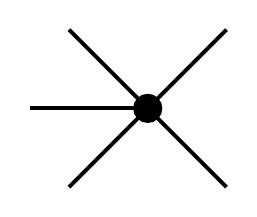
\begin{tikzpicture}
%vertex
\coordinate (b1) at (0,0);
\coordinate (w1) at (-1,1); \coordinate (w2) at (-1.5,0); \coordinate (w3) at (-1,-1);
\coordinate (w5) at (1,1); \coordinate (w6) at (1,-1);
%edge
\draw[line width=0.05cm] (w1)--(b1); \draw[line width=0.05cm] (w2)--(b1);
\draw[line width=0.05cm] (w3)--(b1); \draw[line width=0.05cm] (w5)--(b1); \draw[line width=0.05cm] (w6)--(b1);
%black
\filldraw [line width=0.05cm, fill=black] (b1) circle [radius=0.16] ;
%white
\end{tikzpicture} }} ;

\end{tikzpicture}
}}

\caption{An example of the join and split move.}\label{split_join}
\end{figure}

We sometimes focus on the following type of dimer models.

\begin{Definition}\label{def_hexagonal_square}
We say that a dimer model $\Gamma$ is \emph{hexagonal} (resp.\ \emph{rectangular})
if any face of~$\Gamma$ is hexagon (resp.\ rectangle) and any node of $\Gamma$ is $3$-valent (resp.\ 4-valent).
In particular, a~hexagonal (resp.\ rectangular) dimer model is homotopy-equivalent to a dimer model whose faces are all regular hexagons (resp.\ squares).
\end{Definition}

\subsection{Perfect matchings and the perfect matching polygon}\label{subsection_PM}

Next, we assign a lattice polygon to each dimer model.
For this purpose, we will introduce the notion of perfect matchings, and we construct a polygon called the \emph{perfect matching polygon}.

\begin{Definition}A \emph{perfect matching} (or \emph{dimer configuration}) on a dimer model $\Gamma$ is a subset $\sfP$ of $\Gamma_1$ such that each node is
the end point of precisely one edge in $\sfP$.
\end{Definition}

In general, not every dimer model necessarily has a perfect matching.
In this paper, we will mainly discuss consistent dimer models, and such dimer models have perfect matchings.
Moreover, we can extend a perfect matching $\sfP$ to one on $\widetilde{\Gamma}$ via the universal cover $\RR^2\rightarrow\TT$.
We call this a \emph{perfect matching} on $\widetilde{\Gamma}$, and use the same notation $\sfP$.
For example, some perfect matchings on the dimer model given in Figure~\ref{ex_dimer_4b} are shown in Figure~\ref{pm_4b}.
(This dimer model has eight perfect matchings in total.)

%%% type 4b perfect matching%%%
\begin{figure}[h!]\centering
\newcommand{\edgewidth}{0.07cm}
\newcommand{\nodewidth}{0.07cm}
\newcommand{\noderad}{0.24} %radius_of_node

\newcommand{\pmwidth}{0.5cm}
\newcommand{\pmcolor}{red}

\begin{tikzpicture}
\node at (0,-1.6) {$\sfP_0$};
\node at (3.2,-1.6) {$\sfP_1$}; \node at (6.4,-1.6) {$\sfP_2$}; \node at (9.6,-1.6) {$\sfP_3$}; \node at (12.8,-1.6) {$\sfP_4$};

\node (PM0) at (0,0)
{\scalebox{0.35}{
\begin{tikzpicture}
%perfect matching
\draw[line width=\pmwidth, color=\pmcolor] (W1)--(B3); \draw[line width=\pmwidth, color=\pmcolor] (W3)--(B1);
\draw[line width=\pmwidth, color=\pmcolor] (W2)--(B2);
\basicdimerB
\end{tikzpicture} }};

\node (PM1) at (3.2,0)
{\scalebox{0.35}{
\begin{tikzpicture}
%perfect matching
\draw[line width=\pmwidth, color=\pmcolor] (W3)--(B1);
\draw[line width=\pmwidth, color=\pmcolor] (B3)--(6,3); \draw[line width=\pmwidth, color=\pmcolor] (W2)--(0,3);
\draw[line width=\pmwidth, color=\pmcolor] (W1)--(6,0); \draw[line width=\pmwidth, color=\pmcolor] (B2)--(0,6);
\basicdimerB
\end{tikzpicture} }};

\node (PM2) at (6.4,0)
{\scalebox{0.35}{
\begin{tikzpicture}
%perfect matching
\draw[line width=\pmwidth, color=\pmcolor] (W2)--(B1); \draw[line width=\pmwidth, color=\pmcolor] (W3)--(B3);
\draw[line width=\pmwidth, color=\pmcolor] (W1)--(6,0); \draw[line width=\pmwidth, color=\pmcolor] (B2)--(0,6);
\basicdimerB
\end{tikzpicture} }};

\node (PM3) at (9.6,0)
{\scalebox{0.35}{
\begin{tikzpicture}
%perfect matching
\draw[line width=\pmwidth, color=\pmcolor] (W2)--(B2); \draw[line width=\pmwidth, color=\pmcolor] (W1)--(B3);
\draw[line width=\pmwidth, color=\pmcolor] (W3)--(3,6); \draw[line width=\pmwidth, color=\pmcolor] (B1)--(3,0);
\basicdimerB
\end{tikzpicture} }};

\node (PM4) at (12.8,0)
{\scalebox{0.35}{
\begin{tikzpicture}
%perfect matching
\draw[line width=\pmwidth, color=\pmcolor] (W1)--(B1); \draw[line width=\pmwidth, color=\pmcolor] (W3)--(B2);
\draw[line width=\pmwidth, color=\pmcolor] (B3)--(6,3); \draw[line width=\pmwidth, color=\pmcolor] (W2)--(0,3);
\basicdimerB
\end{tikzpicture} }};

\end{tikzpicture}
\caption{Some perfect matchings on the dimer model given in Figure~\ref{ex_dimer_4b}.}\label{pm_4b}
\end{figure}

We say that a dimer model is \emph{non-degenerate} if every edge is contained in some perfect matchings.
It is known that this non-degeneracy condition is equivalent to the \emph{strong marriage condition}; that is, the dimer model has equal numbers of black and white nodes and every proper subset of the black nodes of size $n$ is connected to at least $n+1$ white nodes (e.g., \cite[Remark~2.12]{Bro}).

Following \cite[Section~5]{IU2}, we next define the perfect matching polygon.
We first fix a perfect matching $\sfP_0$, and call this the \emph{reference perfect matching}.
For any perfect matching $\sfP$, we consider the connected components of the universal cover $\RR^2$ divided by $\sfP\cup\sfP_0$.
Then, we consider the \emph{height function} $\sfh_{\sfP,\sfP_0}$, which is a locally constant function on $\RR^2{\setminus}(\sfP\cup\sfP_0)$, defined as follows.
First, we choose a connected component of $\RR^2{\setminus}(\sfP\cup\sfP_0)$, and define the value of $\sfh_{\sfP,\sfP_0}$ as $0$.
Then, this function increases by $1$ when we cross
\begin{itemize}\itemsep=0pt
\item[--] an edge $e\in\sfP$ with the black node on the right, or
\item[--] an edge $e\in\sfP_0$ with the white node on the right,
\end{itemize}
and decreases by $1$
when we cross
\begin{itemize}\itemsep=0pt
\item[--] an edge $e\in\sfP$ with the white node on the right, or
\item[--] an edge $e\in\sfP_0$ with the black node on the right.
\end{itemize}
This function is determined up to a choice of a connected component of value $0$.
For example, Figure~\ref{fig_heightchnge} shows the height function $\sfh_{\sfP_2,\sfP_3}$ on the dimer model given in Figure~\ref{ex_dimer_4b},
where the red square stands for a fundamental domain of $\TT$, the edges in $\sfP_2$ (resp.~$\sfP_3$) are colored blue (resp.\ green),
and the number filled in each component is the value of $\sfh_{\sfP_2,\sfP_3}$.

\begin{figure}[h!]\centering
\newcommand{\edgewidth}{0.07cm}
\newcommand{\nodewidth}{0.07cm}
\newcommand{\noderad}{0.24} %radius_of_node
\newcommand{\arrowwidth}{0.08cm}
\newcommand{\pmwidth}{0.5cm}

\scalebox{0.33}{
\begin{tikzpicture}
%coordinate setting
\coordinate (W1a) at (5,1); \coordinate (W2a) at (1,3); \coordinate (W3a) at (3,5);
\coordinate (B1a) at (3,1); \coordinate (B2a) at (1,5); \coordinate (B3a) at (5,3);
\coordinate (W1b) at (5,7); \coordinate (W2b) at (1,9); \coordinate (W3b) at (3,11);
\coordinate (B1b) at (3,7); \coordinate (B2b) at (1,11); \coordinate (B3b) at (5,9);
\coordinate (W1c) at (11,1); \coordinate (W2c) at (7,3); \coordinate (W3c) at (9,5);
\coordinate (B1c) at (9,1); \coordinate (B2c) at (7,5); \coordinate (B3c) at (11,3);
\coordinate (W1d) at (11,7); \coordinate (W2d) at (7,9); \coordinate (W3d) at (9,11);
\coordinate (B1d) at (9,7); \coordinate (B2d) at (7,11); \coordinate (B3d) at (11,9);

%perfect matching P2
\draw[line width=\pmwidth, color=blue] (W2a)--(B1a); \draw[line width=\pmwidth, color=blue] (W3a)--(B3a);
\draw[line width=\pmwidth, color=blue] (W1a)--(6,0); \draw[line width=\pmwidth, color=blue] (B2a)--(0,6);
\draw[line width=\pmwidth, color=blue] (W2b)--(B1b); \draw[line width=\pmwidth, color=blue] (W3b)--(B3b);
\draw[line width=\pmwidth, color=blue] (W1b)--(B2c); \draw[line width=\pmwidth, color=blue] (B2b)--(0,12);
\draw[line width=\pmwidth, color=blue] (W2c)--(B1c); \draw[line width=\pmwidth, color=blue] (W3c)--(B3c);
\draw[line width=\pmwidth, color=blue] (W1c)--(12,0); \draw[line width=\pmwidth, color=blue] (B2c)--(6,6);
\draw[line width=\pmwidth, color=blue] (W2d)--(B1d); \draw[line width=\pmwidth, color=blue] (W3d)--(B3d);
\draw[line width=\pmwidth, color=blue] (W1d)--(12,6); \draw[line width=\pmwidth, color=blue] (B2d)--(6,12);

%perfect matching P3
\draw[line width=\pmwidth, color=green] (W2a)--(B2a); \draw[line width=\pmwidth, color=green] (W1a)--(B3a);
\draw[line width=\pmwidth, color=green] (W3a)--(B1b); \draw[line width=\pmwidth, color=green] (B1a)--(3,0);
\draw[line width=\pmwidth, color=green] (W2b)--(B2b); \draw[line width=\pmwidth, color=green] (W1b)--(B3b);
\draw[line width=\pmwidth, color=green] (W3b)--(3,12);
\draw[line width=\pmwidth, color=green] (W2c)--(B2c); \draw[line width=\pmwidth, color=green] (W1c)--(B3c);
\draw[line width=\pmwidth, color=green] (W3c)--(B1d); \draw[line width=\pmwidth, color=green] (B1c)--(9,0);
\draw[line width=\pmwidth, color=green] (W2d)--(B2d); \draw[line width=\pmwidth, color=green] (W1d)--(B3d);
\draw[line width=\pmwidth, color=green] (W3d)--(9,12);

%edge
\draw[line width=\edgewidth] (W2a)--(B1a)--(W1a)--(B3a)--(W3a)--(B2a)--(W2a); \draw[line width=\edgewidth] (B1a)--(W3a);
\draw[line width=\edgewidth] (0,3)--(W2a); \draw[line width=\edgewidth] (3,0)--(B1a); \draw[line width=\edgewidth] (6,0)--(W1a);
\draw[line width=\edgewidth] (0,6)--(B2a);
\draw[line width=\edgewidth] (W2b)--(B1b)--(W1b)--(B3b)--(W3b)--(B2b)--(W2b); \draw[line width=\edgewidth] (B1b)--(W3b);
\draw[line width=\edgewidth] (0,9)--(W2b); \draw[line width=\edgewidth] (0,12)--(B2b); \draw[line width=\edgewidth] (3,12)--(W3b);
\draw[line width=\edgewidth] (W2c)--(B1c)--(W1c)--(B3c)--(W3c)--(B2c)--(W2c); \draw[line width=\edgewidth] (B1c)--(W3c);
\draw[line width=\edgewidth] (9,0)--(B1c); \draw[line width=\edgewidth] (12,0)--(W1c); \draw[line width=\edgewidth] (12,3)--(B3c);
\draw[line width=\edgewidth] (W2d)--(B1d)--(W1d)--(B3d)--(W3d)--(B2d)--(W2d); \draw[line width=\edgewidth] (B1d)--(W3d);
\draw[line width=\edgewidth] (12,6)--(W1d);\draw[line width=\edgewidth] (6,12)--(B2d);
\draw[line width=\edgewidth] (12,9)--(B3d); \draw[line width=\edgewidth] (9,12)--(W3d);
\draw[line width=\edgewidth] (W3a)--(B1b); \draw[line width=\edgewidth] (B3a)--(W2c);
\draw[line width=\edgewidth] (B3b)--(W2d); \draw[line width=\edgewidth] (B2c)--(W1b);
\draw[line width=\edgewidth] (W3c)--(B1d);

%black
\draw [line width=\nodewidth, fill=black] (B1a) circle [radius=\noderad] ;
\draw [line width=\nodewidth, fill=black] (B2a) circle [radius=\noderad] ;
\draw [line width=\nodewidth, fill=black] (B3a) circle [radius=\noderad] ;
\draw [line width=\nodewidth, fill=black] (B1b) circle [radius=\noderad] ;
\draw [line width=\nodewidth, fill=black] (B2b) circle [radius=\noderad] ;
\draw [line width=\nodewidth, fill=black] (B3b) circle [radius=\noderad] ;
\draw [line width=\nodewidth, fill=black] (B1c) circle [radius=\noderad] ;
\draw [line width=\nodewidth, fill=black] (B2c) circle [radius=\noderad] ;
\draw [line width=\nodewidth, fill=black] (B3c) circle [radius=\noderad] ;
\draw [line width=\nodewidth, fill=black] (B1d) circle [radius=\noderad] ;
\draw [line width=\nodewidth, fill=black] (B2d) circle [radius=\noderad] ;
\draw [line width=\nodewidth, fill=black] (B3d) circle [radius=\noderad] ;
%white
\draw [line width=\nodewidth, fill=white] (W1a) circle [radius=\noderad] ;
\draw [line width=\nodewidth, fill=white] (W2a) circle [radius=\noderad] ;
\draw [line width=\nodewidth, fill=white] (W3a) circle [radius=\noderad] ;
\draw [line width=\nodewidth, fill=white] (W1b) circle [radius=\noderad] ;
\draw [line width=\nodewidth, fill=white] (W2b) circle [radius=\noderad] ;
\draw [line width=\nodewidth, fill=white] (W3b) circle [radius=\noderad] ;
\draw [line width=\nodewidth, fill=white] (W1c) circle [radius=\noderad] ;
\draw [line width=\nodewidth, fill=white] (W2c) circle [radius=\noderad] ;
\draw [line width=\nodewidth, fill=white] (W3c) circle [radius=\noderad] ;
\draw [line width=\nodewidth, fill=white] (W1d) circle [radius=\noderad] ;
\draw [line width=\nodewidth, fill=white] (W2d) circle [radius=\noderad] ;
\draw [line width=\nodewidth, fill=white] (W3d) circle [radius=\noderad] ;

%height
\node at (1,1) {\Huge$\mathchar`-1$}; \node at (0.35,4) {\Huge$\mathchar`-1$};
\node at (2,3.5) {\Huge$0$}; \node at (4,2.5) {\Huge$0$}; \node at (4,0.5) {\Huge$0$}; \node at (1,7) {\Huge$0$}; \node at (0.35,10) {\Huge$0$};
\node at (5,5) {\Huge$1$}; \node at (7,1) {\Huge$1$}; \node at (4,8.5) {\Huge$1$}; \node at (2,9.5) {\Huge$1$}; \node at (2,11.65) {\Huge$1$};
\node at (10,0.5) {\Huge$2$}; \node at (8,3.5) {\Huge$2$}; \node at (10,2.5) {\Huge$2$}; \node at (7,7) {\Huge$2$}; \node at (5,11) {\Huge$2$};
\node at (11.65,2) {\Huge$3$}; \node at (11,5) {\Huge$3$}; \node at (8,9.5) {\Huge$3$}; \node at (10,8.5) {\Huge$3$}; \node at (8,11.65) {\Huge$3$};
\node at (11,11) {\Huge$4$}; \node at (11.65,8) {\Huge$4$};

%fundamental domain
\draw[line width=0.12cm, red] (0,0) rectangle (6,6);
\end{tikzpicture}
}
\caption{The height function $\sfh_{\sfP_2,\sfP_3}$.}\label{fig_heightchnge}
\end{figure}

We then take a point $\pt\in\RR^2{\setminus}(\sfP\cup\sfP_0)$, and define the \emph{height change}
\begin{displaymath}
h(\sfP,\sfP_0)=(h_x(\sfP,\sfP_0),h_y(\sfP,\sfP_0))\in\ZZ^2
\end{displaymath}
of $\sfP$ with respect to $\sfP_0$ as the differences of the height function:
\begin{gather*}
h_x(\sfP,\sfP_0)=\sfh_{\sfP,\sfP_0}(\pt+(1,0))-\sfh_{\sfP,\sfP_0}(\pt),
\\
h_y(\sfP,\sfP_0)=\sfh_{\sfP,\sfP_0}(\pt+(0,1))-\sfh_{\sfP,\sfP_0}(\pt).
\end{gather*}
We remark that this does not depend on the choice of $\pt\in\RR^2{\setminus}(\sfP\cup\sfP_0)$.
We then consider the height change $h(\sfP,\sfP^\prime)$ for any pair of perfect matchings $\sfP$, $\sfP^\prime$,
but since we have
\begin{equation*}%\label{relation_height}
h(\sfP,\sfP^\prime)=h(\sfP,\sfP_0)-h(\sfP^\prime,\sfP_0),
\end{equation*}
it is enough to consider height changes with respect to the reference perfect matching $\sfP_0$.
Then, the \emph{perfect matching} (= \emph{PM}) \emph{polygon} (or \emph{characteristic polygon}) $\Delta_\Gamma\subset\RR^2$ of a dimer model $\Gamma$ is defined
as the convex hull of $\big\{h(\sfP,\sfP_0)\in\ZZ^2\,|\, \sfP\in\PM(\Gamma)\big\}$ where $\PM(\Gamma)$ is the set of perfect matchings on~$\Gamma$.

\begin{Remark}\label{rem_polygon}
The description of height changes depends on the choice of the coordinate system fixed in $\TT$
(i.e., the choice of a fundamental domain).
A change of a coordinate system induces a $\GL(2,\ZZ)$-action on the PM polygon, and this action does not affect our problem.
In the following, we say that two polygons $P$ and $Q$ are \emph{$\GL(2,\ZZ)$-equivalent} if they are transformed into each other by $\GL(2,\ZZ)$-transformations, in which case we denote $P\cong Q$.
Thus, we may fix some fundamental domain of~$\TT$.
Also, we remark that the description of the polygon $\Delta_\Gamma$ depends on the choice of a reference perfect matching, but it is determined up to translations.
\end{Remark}

\begin{Definition}\label{def_corner}
Fix a perfect matching $\sfP_0$ and let $\Delta_\Gamma$ be the perfect matching polygon.
We say that a perfect matching $\sfP$ is
\begin{itemize}\itemsep=0pt
\item a \emph{corner} (or \emph{extremal}) \emph{perfect matching} if $h(\sfP,\sfP_0)$ is a vertex of $\Delta_\Gamma$,
\item a \emph{boundary} (or \emph{external}) \emph{perfect matching} if $h(\sfP,\sfP_0)$ is a lattice point on an edge of $\Delta_\Gamma$
(in particular, corner perfect matchings are boundary perfect matchings),
\item an \emph{internal} \emph{perfect matching} if $h(\sfP,\sfP_0)$ is an interior lattice point of $\Delta_\Gamma$.
\end{itemize}
\end{Definition}

In the next subsection, we will introduce consistent dimer models (see Definition~\ref{def_consistent}), which have several nice properties.
If a dimer model is consistent, then there exists a unique corner perfect matching corresponding to each vertex of $\Delta_\Gamma$
(e.g., \cite[Corollary~4.27]{Bro}, \cite[Proposition~9.2]{IU2}).
Thus, we can give a cyclic order to corner perfect matchings along the corresponding vertices of $\Delta_\Gamma$ in the anti-clockwise direction.
We say that two corner perfect matchings are \emph{adjacent} if they are adjacent with respect to the given cyclic order.

\begin{Example}
We consider the dimer model given in Figure~\ref{ex_dimer_4b}, which is consistent as we will see in the next subsection.
Fix the perfect matching $\sfP_0$ shown in Figure~\ref{pm_4b} as the reference one.
Then, we see that the perfect matchings $\sfP_1,\dots,\sfP_4$ correspond to lattice points $(1,0)$, $(1,1)$, $(-1,0)$, $(0,-1)$, respectively.
Since $\sfP_0$ is the reference perfect matching, it corresponds to $(0,0)$.
In addition, this dimer model has three perfect matchings that are not listed in Figure~\ref{pm_4b},
and such perfect matchings also correspond to $(0,0)$.
Thus, the PM polygon takes the form shown in Figure~\ref{polygon_4b}, and hence $\sfP_1,\dots,\sfP_4$ are corner perfect matchings.

\begin{figure}[h!]\centering
\scalebox{0.75}{
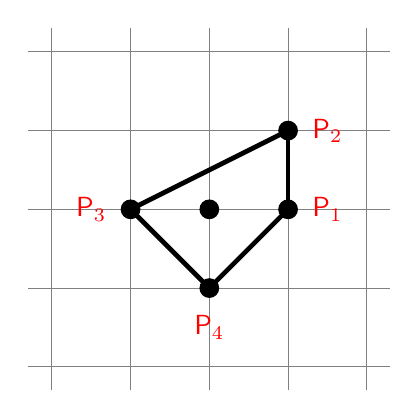
\begin{tikzpicture}
\coordinate (00) at (0,0); \coordinate (10) at (1,0); \coordinate (01) at (0,1); \coordinate (-10) at (-1,0); \coordinate (11) at (1,1);
\coordinate (0-1) at (0,-1);

\draw [step=1, gray] (-2.3,-2.3) grid (2.3,2.3);
\draw [line width=0.06cm] (10)--(11) ; \draw [line width=0.06cm] (11)--(-10) ;
\draw [line width=0.06cm] (-10)--(0-1) ; \draw [line width=0.06cm] (0-1)--(10) ;

\draw [line width=0.05cm, fill=black] (00) circle [radius=0.1] ; \draw [line width=0.05cm, fill=black] (10) circle [radius=0.1] ;
\draw [line width=0.05cm, fill=black] (11) circle [radius=0.1] ;
\draw [line width=0.05cm, fill=black] (-10) circle [radius=0.1] ; \draw [line width=0.05cm, fill=black] (0-1) circle [radius=0.1] ;

\node [red] at (1.5,0) {$\sfP_1$} ;
\node [red] at (1.5,1) {$\sfP_2$} ; \node [red] at (-1.5,0) {$\sfP_3$} ;
\node [red] at (0,-1.5) {$\sfP_4$} ;

\end{tikzpicture}
}
\caption{The PM polygon of the dimer model given in Figure~\ref{ex_dimer_4b}.}\label{polygon_4b}
\end{figure}
\end{Example}

In this way, we can obtain the PM polygon from a dimer model.
On the other hand, it is known that any lattice polygon can be obtained as the PM polygon of a certain dimer model.

\begin{Theorem}[\cite{Gul,IU2}]\label{existence_dimer}
For any lattice polygon $\Delta$ in $\RR^2$, there exists a dimer model $\Gamma$ giving $\Delta$ as the PM polygon $\Delta_\Gamma$.
Furthermore, we can take this $\Gamma$ as it satisfies the consistency condition $($see Definition~{\rm \ref{def_consistent})}.
\end{Theorem}

Thus, for a given lattice polygon $\Delta$, we say that $\Gamma$ is a \emph{dimer model associated with $\Delta$} if the PM polygon of~$\Gamma$ coincides with~$\Delta$.
We remark that for a given polygon $\Delta$, the associated consistent dimer model is not unique in general.

\section{Zigzag paths and their properties}\label{sec_zigzag}

\subsection{Consistency conditions}\label{subsec_consistency}

In this subsection, we introduce the consistency condition.
In order to define this condition, we first introduce the notion of zigzag paths.
These paths are also the main ingredients for introducing deformations of dimer models.

\begin{Definition}We say that a path on a dimer model is a \emph{zigzag path} if it makes a maximum turn to the right on a white node and a maximum turn to the left on a black node.
Also, we say that a zigzag path is \emph{reduced} if it does not pass through $2$-valent nodes.
(We remark that we can make a zigzag path reduced using the join moves. In particular, any zigzag path on a~reduced dimer model is reduced.)
\end{Definition}

Since a dimer model has only finitely many edges, we see that all zigzag paths are periodic.
For a zigzag path $z$ on $\Gamma$, we define the length of~$z$, which is denoted by~$\ell(z)$, as the number of edges of~$\Gamma$ constituting~$z$.
In particular, we see that $\ell(z)$ is an even integer.
Thus, edges on a~zigzag path are indexed by elements in $\ZZ/(2n)\ZZ$ for some integer $\ell(z)/2=n\ge 1$.
Fix a black node on a zigzag path $z$ as the starting point of~$z$, and denote~$z$ as a sequence of edges starting from the fixed black node:
$z=z[1]z[2]\cdots z[2n-1]z[2n]$.

\begin{center}
{\scalebox{0.7}{
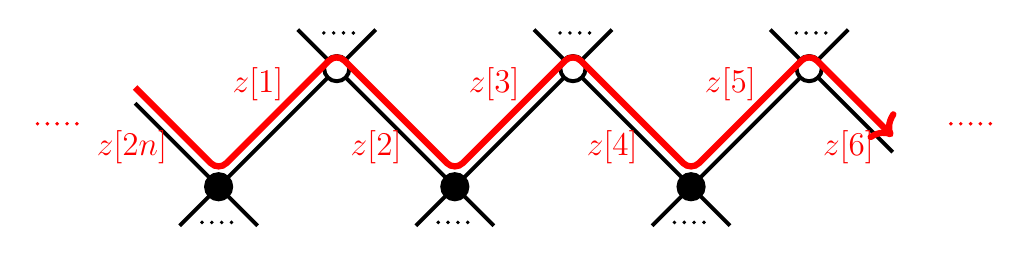
\begin{tikzpicture}
\newcommand{\edgewidth}{0.05cm} %line_width_of _edges
\newcommand{\nodewidth}{0.05cm} %line_width_around_nodes
\newcommand{\noderad}{0.16} %radius_of_node

%coordinate setting
\coordinate (B1) at (0,0); \coordinate (B2) at (3,0); \coordinate (B3) at (6,0);
\coordinate (W1) at (1.5,1.5); \coordinate (W2) at (4.5,1.5); \coordinate (W3) at (7.5,1.5);

\path (B1) ++(135:1.5cm) coordinate (B1w); \path (B1) ++(225:0.7cm) coordinate (B1s); \path (B1) ++(315:0.7cm) coordinate (B1e);
\path (W1) ++(45:0.7cm) coordinate (W1w); \path (W1) ++(135:0.7cm) coordinate (W1s);
\path (B2) ++(225:0.7cm) coordinate (B2s); \path (B2) ++(315:0.7cm) coordinate (B2e);
\path (W2) ++(45:0.7cm) coordinate (W2w); \path (W2) ++(135:0.7cm) coordinate (W2s);
\path (B3) ++(225:0.7cm) coordinate (B3s); \path (B3) ++(315:0.7cm) coordinate (B3e);
\path (W3) ++(315:1.5cm) coordinate (W3n); \path (W3) ++(45:0.7cm) coordinate (W3w); \path (W3) ++(135:0.7cm) coordinate (W3s);

\path (B1) ++(245:0.5cm) coordinate (B1ss); \path (B1) ++(295:0.5cm) coordinate (B1ee);
\path (W1) ++(65:0.5cm) coordinate (W1ww); \path (W1) ++(115:0.5cm) coordinate (W1ss);
\path (B2) ++(245:0.5cm) coordinate (B2ss); \path (B2) ++(295:0.5cm) coordinate (B2ee);
\path (W2) ++(65:0.5cm) coordinate (W2ww); \path (W2) ++(115:0.5cm) coordinate (W2ss);
\path (B3) ++(245:0.5cm) coordinate (B3ss); \path (B3) ++(295:0.5cm) coordinate (B3ee);
\path (W3) ++(65:0.5cm) coordinate (W3ww); \path (W3) ++(115:0.5cm) coordinate (W3ss);
%edge
\draw [line width=\edgewidth] (B1w)--(B1)--(W1)--(B2)--(W2)--(B3)--(W3)--(W3n);
\draw [line width=\edgewidth] (B1s)--(B1)--(B1e); \draw[line width=\edgewidth] (B2s)--(B2)--(B2e); \draw [line width=\edgewidth] (B3s)--(B3)--(B3e);
\draw [line width=\edgewidth] (W1w)--(W1)--(W1s); \draw[line width=\edgewidth] (W2w)--(W2)--(W2s); \draw [line width=\edgewidth] (W3w)--(W3)--(W3s);

\draw [line width=\edgewidth,line cap=round, dash pattern=on 0pt off 2.5\pgflinewidth] (B1ss)--(B1ee);
\draw [line width=\edgewidth,line cap=round, dash pattern=on 0pt off 2.5\pgflinewidth] (W1ww)--(W1ss);
\draw [line width=\edgewidth,line cap=round, dash pattern=on 0pt off 2.5\pgflinewidth] (B2ss)--(B2ee);
\draw [line width=\edgewidth,line cap=round, dash pattern=on 0pt off 2.5\pgflinewidth] (W2ww)--(W2ss);
\draw [line width=\edgewidth,line cap=round, dash pattern=on 0pt off 2.5\pgflinewidth] (B3ss)--(B3ee);
\draw [line width=\edgewidth,line cap=round, dash pattern=on 0pt off 2.5\pgflinewidth] (W3ww)--(W3ss);
%blacknode
\draw [line width=\nodewidth, fill=black] (B1) circle [radius=\noderad] ;
\draw [line width=\nodewidth, fill=black] (B2) circle [radius=\noderad] ;
\draw [line width=\nodewidth, fill=black] (B3) circle [radius=\noderad] ;
%whitenode
\draw [line width=\nodewidth, fill=white] (W1) circle [radius=\noderad] ;
\draw [line width=\nodewidth, fill=white] (W2) circle [radius=\noderad] ;
\draw [line width=\nodewidth, fill=white] (W3) circle [radius=\noderad] ;
%zigzag
\path (B1w) ++(90:0.2cm) coordinate (B1w+);
\path (B1) ++(90:0.2cm) coordinate (B1+); \path (W1) ++(90:0.2cm) coordinate (W1+);
\path (B2) ++(90:0.2cm) coordinate (B2+); \path (W2) ++(90:0.2cm) coordinate (W2+);
\path (B3) ++(90:0.2cm) coordinate (B3+); \path (W3) ++(90:0.2cm) coordinate (W3+);
\path (W3n) ++(90:0.2cm) coordinate (W3n+);
\draw [->, rounded corners, line width=0.08cm, red] (B1w+)--(B1+)--(W1+)--(B2+)--(W2+)--(B3+)--(W3+)--(W3n+) ;
\draw [line width=0.05cm, red, line cap=round, dash pattern=on 0pt off 2.5\pgflinewidth] (-1.8,0.8)--(-2.4,0.8) ;
\draw [line width=0.05cm, red, line cap=round, dash pattern=on 0pt off 2.5\pgflinewidth] (9.3,0.8)--(9.9,0.8) ;
%index
\node[red] at (0.5,1.3) {\large$z[1]$} ; \node[red] at (2,0.5) {\large$z[2]$} ;
\node[red] at (3.5,1.3) {\large$z[3]$} ; \node[red] at (5,0.5) {\large$z[4]$} ;
\node[red] at (6.5,1.3) {\large$z[5]$} ; \node[red] at (8,0.5) {\large$z[6]$} ;
\node[red] at (-1.1,0.5) {\large$z[2n]$} ;
\end{tikzpicture}
} }
\end{center}

An edge in a zigzag path $z$ is called a \emph{zig} (resp.\ \emph{zag}) of $z$ if it is indexed by an odd (resp.~even) integer.
We denote by $\Zig(z)$ (resp.~$\Zag(z)$) the set of zigs (resp.~zags) appearing in a~zigzag path~$z$, which is a~finite set.
Two zigzag paths are said to \emph{intersect} if they share an edge (not a node).
We note that if $z$ does not have a self-intersection, $\Zig(z)$ and $\Zag(z)$ are disjoint sets.
For any edge~$e$ of a dimer model, we can consider the zigzag path containing $e$ as a zig and the zigzag path containing $e$ as a zag.
Thus, any edge $e$ is contained in at most two zigzag paths.
If such zigzag paths do not have a self-intersection, $e$ is contained in exactly two zigzag paths.
For example, zigzag paths on the dimer model given in the left of Figure~\ref{ex_dimer_4b} are shown in Figure~\ref{zigzag_4b}.

\begin{figure}[h!]
\centering

\newcommand{\edgewidth}{0.07cm}
\newcommand{\nodewidth}{0.07cm}
\newcommand{\noderad}{0.24} %radius_of_node

{\scalebox{1}{
\begin{tikzpicture}

\node at (0,-1.6) {$z_1$}; \node at (3.5,-1.6) {$z_2$}; \node at (7,-1.6) {$z_3$}; \node at (10.5,-1.6) {$z_4$};

\node (ZZ1) at (0,0)
{\scalebox{0.4}{
\begin{tikzpicture}
\basicdimerB
%zigzag path
\draw[->, line width=0.2cm, rounded corners, color=red] (0,3)--(W2)--(B1)--(W3)--(B3)--(6,3);
\end{tikzpicture} }};

\node (ZZ2) at (3.5,0)
{\scalebox{0.4}{
\begin{tikzpicture}
\basicdimerB
%zigzag path
\draw[->, line width=0.2cm, rounded corners, color=red] (3,0)--(B1)--(W2)--(B2)--(0,6);
\draw[->, line width=0.2cm, rounded corners, color=red] (6,0)--(W1)--(B3)--(W3)--(3,6);
\end{tikzpicture} }} ;

\node (ZZ3) at (7,0)
{\scalebox{0.4}{
\begin{tikzpicture}
\basicdimerB
%zigzag path
\draw[->, line width=0.2cm, rounded corners, color=red] (3,6)--(W3)--(B2)--(W2)--(0,3);
\draw[->, line width=0.2cm, rounded corners, color=red] (6,3)--(B3)--(W1)--(B1)--(3,0);
\end{tikzpicture} }};

\node (ZZ4) at (10.5,0)
{\scalebox{0.4}{
\begin{tikzpicture}
\basicdimerB
%zigzag path
\draw[->, line width=0.2cm, rounded corners, color=red] (0,6)--(B2)--(W3)--(B1)--(W1)--(6,0);
\end{tikzpicture} }} ;

\end{tikzpicture}
}}
\caption{All zigzag paths on the dimer model given in Figure~\ref{ex_dimer_4b}.}\label{zigzag_4b}
\end{figure}

For a zigzag path $z$ on a dimer model $\Gamma$, we also consider the lift of $z$ to the universal cover~$\widetilde{\Gamma}$.
Let $\widetilde{z}{(\alpha)}$ denote a zigzag path on $\widetilde{\Gamma}$ whose projection on $\Gamma$ is $z$ where $\alpha\in\ZZ$.
When we do not need to specify these, we simply denote each of them by~$\widetilde{z}$.
Then, we see that a zigzag path on~$\widetilde{\Gamma}$ is either periodic or infinite in both directions.
Using these notions, we introduce the consistency condition.

\begin{Definition}[{see \cite[Definition~3.5]{IU1}}]
\label{def_consistent}
We say that a dimer model is (\emph{zigzag}) \emph{consistent} if it satisfies the following conditions:
\begin{itemize}\itemsep=0pt
\item [(1)] there is no homologically trivial zigzag path,
\item [(2)] no zigzag path on the universal cover has a self-intersection,
\item [(3)] no pair of zigzag paths on the universal cover intersect each other in the same direction more than once.
That is, if a pair of zigzag paths $(\widetilde{z},\widetilde{w})$ on the universal cover has two intersected edges $a_1$, $a_2$
and $\widetilde{z}$ points from $a_1$ to $a_2$, then $\widetilde{w}$ points from $a_2$ to $a_1$.
\end{itemize}
\end{Definition}

In the literature, there are several conditions that are equivalent to Definition~\ref{def_consistent} (for more details, see \cite{Boc1,IU1}),
and it is known that a consistent dimer model is non-degenerate (e.g., \cite[Proposition~8.1]{IU2}).
For example, we see that the dimer model given in Figure~\ref{ex_dimer_4b} is consistent by checking all zigzag paths, which are shown in Figure~\ref{zigzag_4b}.
We also remark that this dimer model satisfies the stronger condition called \emph{isoradial} (see Definition~\ref{def_isoradial}).

In this paper, we also use another condition called \emph{properly ordered}.
To explain the proper ordering, we prepare several notation.
First, considering a zigzag path $z$ as a $1$-cycle on $\TT$, we have the homology class $[z]\in\rmH_1(\TT)\cong\ZZ^2$. We call this element $[z]\in\ZZ^2$ the \emph{slope} of $z$.
We remark that even if we apply the join and split moves to nodes contained in a zigzag path, such operations do not change the slope.
If a zigzag path does not have any self-intersection, the slope of each zigzag path is primitive.
Now, we consider slopes $(a,b)\in\ZZ^2$ of zigzag paths that are not homologically trivial.
The set of such slopes has a natural cyclic order by considering~$(a,b)$ as an element of the unit circle:
\begin{displaymath}
\frac{(a,b)}{\sqrt{a^2+b^2}}\in S^1.
\end{displaymath}
We say that two zigzag paths are \emph{adjacent} if their slopes are adjacent with respect to the above cyclic order.
Using this cyclic order, we define a properly ordered dimer model below.
In particular, it is known that a dimer model is consistent in the sense of Definition~\ref{def_consistent} if and only if it is properly ordered (see \cite[Proposition~4.4]{IU1}).

\begin{Definition}[{see \cite[Section~3.1]{Gul}}]\label{def_properly}
A dimer model is said to be \emph{properly ordered} if
\begin{itemize}\itemsep=0pt
\item [(1)] there is no homologically trivial zigzag path,
\item [(2)] no zigzag path on the universal cover has a self-intersection,
\item [(3)] no pair of zigzag paths with the same slope have a common node,
\item [(4)] for any node on the dimer model, the natural cyclic order on the set of zigzag paths incident to that node
coincides with the cyclic order determined by their slopes.
\end{itemize}
\end{Definition}

We also introduce isoradial dimer models which are stronger than consistent ones.
The dimer model given in Figure~\ref{ex_dimer_4b} is isoradial in particular.

\begin{Definition}[{\cite[Theorem~5.1]{KS}; see also \cite{Duf,Mer}}]
\label{def_isoradial}
We say that a dimer model $\Gamma$ is \emph{isoradial} (or \emph{geometrically consistent}) if
\begin{itemize}\itemsep=0pt
\item [(1)] every zigzag path is a simple closed curve,
\item [(2)] any pair of zigzag paths on the universal cover share at most one edge.
\end{itemize}
\end{Definition}

\subsection{Relationships between perfect matchings and zigzag paths}\label{subsec_relation_zigzag_pm}

We can now discuss the relationship between perfect matchings and zigzag paths.
The following proposition is essential throughout this paper.

\begin{Proposition}[{see \cite[Theorem~3.3 and Corollary~3.8]{Gul}, \cite[Proposition~9.2 and Corollary~9.3]{IU2}}]\label{zigzag_sidepolygon}
There exists a one-to-one correspondence between the set of slopes of zigzag paths on a consistent dimer model $\Gamma$ and
the set of primitive side segments of the PM polygon $\Delta_\Gamma$. More precisely, each slope of a zigzag path is the primitive outer normal vector for a primitive side segment of~$\Delta_\Gamma$.

Moreover, zigzag paths having the same slope arise as the difference of two adjacent corner perfect matchings $\sfP$, $\sfP^\prime$ $($i.e., the edges in $\sfP\cup\sfP^\prime{\setminus}\sfP\cap\sfP^\prime$ form zigzag paths$)$. Thus, any corner perfect matching intersects with half of the edges constituting a certain zigzag path.
\end{Proposition}

For example, the zigzag path $z_1$ shown in Figure~\ref{zigzag_4b} is obtained from the pair of adjacent corner perfect matchings $(\sfP_1,\sfP_2)$ given in Figure~\ref{pm_4b}. Also, the zigzag paths $z_2$, $z_3$, $z_4$ are obtained by pairs $(\sfP_2,\sfP_3)$, $(\sfP_3,\sfP_4)$, $(\sfP_4,\sfP_1)$, respectively.

By Proposition~\ref{zigzag_sidepolygon}, we can assign each edge of the PM polygon to a zigzag path~$z$;
thus we will call this the edge corresponding to~$z$.
In particular, the edges corresponding to zigzag paths having the same slope are all the same.

Let $\sfP$, $\sfP^\prime$ be adjacent corner perfect matchings on a consistent dimer model, and $z_1,\dots, z_r$ be the zigzag paths arising from $\sfP$ and $\sfP^\prime$ as in Proposition~\ref{zigzag_sidepolygon}.
In particular, these zigzag paths have the same slope.
We see that $\sfP\cap z_i=\Zig(z_i)$ and $\sfP^\prime\cap z_i=\Zag(z_i)$ (or $\sfP\cap z_i=\Zag(z_i)$ and $\sfP^\prime\cap z_i=\Zig(z_i)$) for any $i=1,\dots,r$. Here, $\sfP\cap z_i$ denotes the subset of edges in $\sfP$ contained in~$z_i$.
Then, we have the description of boundary perfect matchings using the corner ones.

\begin{Proposition}[{e.g., \cite[Proposition~4.35]{Bro}, \cite[Corollary~3.8]{Gul}}]\label{char_bound}
Let $\sfP$, $\sfP^\prime$ and $z_1,\dots, z_r$ be as above.
Let $E$ be the edge of the PM polygon of $\Gamma$ corresponding to $z_1,\dots, z_r$.
We assume that $\sfP\cap z_i=\Zig(z_i)$ and $\sfP^\prime\cap z_i=\Zag(z_i)$.
Then, any boundary perfect matching corresponding to a~lattice point on $E$ can be described as
\begin{displaymath}
\bigg(\sfP{\setminus}\bigcup_{i\in I}\Zig(z_i)\bigg)\cup\bigcup_{i\in I}\Zag(z_i) \qquad or \qquad \bigg(\sfP^\prime{\setminus}\bigcup_{i\in I}\Zag(z_i)\bigg)\cup\bigcup_{i\in I}\Zig(z_i),
\end{displaymath}
where $I$ is a subset of $\{1, \dots, r\}$.
In particular, the number of perfect matchings corresponding to a~lattice point~$\mathsf{q}$ on~$E$ is~$\dbinom{r}{m}$,
where~$m$ is the number of primitive side segments of~$E$ between~$\mathsf{q}$ and one of the endpoints of~$E$.
\end{Proposition}

We then observe the relationships between zigzag paths and height changes of perfect matchings.
Some of these relationships are well-known to experts, but we will consider them in detail because these statements are quite important
when we define the deformation of consistent dimer models in Section~\ref{sec_def_deform}, and also for the self-containedness.

\begin{observation}[{cf.~\cite[Section~5.3]{IU2}}]\label{height_zigzag}
Let $\Gamma$ be a consistent dimer model.
For any zigzag path~$z$, the slope $[z]$ is an element in $\rmH_1(\TT)$.
On the other hand, we can consider height changes as elements in the cohomology group $\rmH^1(\TT)\cong\ZZ^2$.
We consider a pairing \mbox{$\langle{-},{-}\rangle\colon \! \rmH^1(\TT)\!\times\!\rmH_1(\TT)\!\rightarrow\!\ZZ$}.
By Propositions~\ref{zigzag_sidepolygon} and \ref{char_bound}, there is a perfect matching $\sfP^\prime$ that intersects half of the edges constituting~$z$.
Then, for any perfect matching $\sfP$, we have $\langle h(\sfP,\sfP^\prime),[z]\rangle\le 0$.
In fact, we first replace~$z$ by the path~$p_z$ on the quiver $Q_\Gamma$ going along the left side of~$z$ (see the figure below).

\begin{center}
{\scalebox{0.6}{
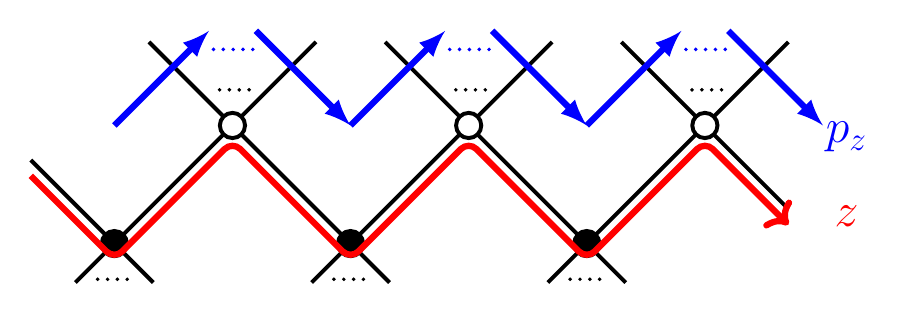
\begin{tikzpicture}[sarrow/.style={black, -latex, very thick},tarrow/.style={black, latex-, very thick}]
\newcommand{\edgewidth}{0.05cm} %line_width_of _edges
\newcommand{\nodewidth}{0.05cm} %line_width_around_nodes
\newcommand{\noderad}{0.16} %radius_of_node

%coordinate setting
\coordinate (B1) at (0,0); \coordinate (B2) at (3,0); \coordinate (B3) at (6,0);
\coordinate (W1) at (1.5,1.5); \coordinate (W2) at (4.5,1.5); \coordinate (W3) at (7.5,1.5);

\path (B1) ++(135:1.5cm) coordinate (B1w); \path (B1) ++(225:0.7cm) coordinate (B1s); \path (B1) ++(315:0.7cm) coordinate (B1e);
\path (W1) ++(45:1.5cm) coordinate (W1w); \path (W1) ++(135:1.5cm) coordinate (W1s);
\path (B2) ++(225:0.7cm) coordinate (B2s); \path (B2) ++(315:0.7cm) coordinate (B2e);
\path (W2) ++(45:1.5cm) coordinate (W2w); \path (W2) ++(135:1.5cm) coordinate (W2s);
\path (B3) ++(225:0.7cm) coordinate (B3s); \path (B3) ++(315:0.7cm) coordinate (B3e);
\path (W3) ++(315:1.5cm) coordinate (W3n); \path (W3) ++(45:1.5cm) coordinate (W3w); \path (W3) ++(135:1.5cm) coordinate (W3s);

\path (B1) ++(245:0.5cm) coordinate (B1ss); \path (B1) ++(295:0.5cm) coordinate (B1ee);
\path (W1) ++(65:0.5cm) coordinate (W1ww); \path (W1) ++(115:0.5cm) coordinate (W1ss);
\path (B2) ++(245:0.5cm) coordinate (B2ss); \path (B2) ++(295:0.5cm) coordinate (B2ee);
\path (W2) ++(65:0.5cm) coordinate (W2ww); \path (W2) ++(115:0.5cm) coordinate (W2ss);
\path (B3) ++(245:0.5cm) coordinate (B3ss); \path (B3) ++(295:0.5cm) coordinate (B3ee);
\path (W3) ++(65:0.5cm) coordinate (W3ww); \path (W3) ++(115:0.5cm) coordinate (W3ss);
%edge
\draw [line width=\edgewidth] (B1w)--(B1)--(W1)--(B2)--(W2)--(B3)--(W3)--(W3n);
\draw [line width=\edgewidth] (B1s)--(B1)--(B1e); \draw[line width=\edgewidth] (B2s)--(B2)--(B2e); \draw [line width=\edgewidth] (B3s)--(B3)--(B3e);
\draw [line width=\edgewidth] (W1w)--(W1)--(W1s); \draw[line width=\edgewidth] (W2w)--(W2)--(W2s); \draw [line width=\edgewidth] (W3w)--(W3)--(W3s);

\draw [line width=\edgewidth,line cap=round, dash pattern=on 0pt off 2.5\pgflinewidth] (B1ss)--(B1ee);
\draw [line width=\edgewidth,line cap=round, dash pattern=on 0pt off 2.5\pgflinewidth] (W1ww)--(W1ss);
\draw [line width=\edgewidth,line cap=round, dash pattern=on 0pt off 2.5\pgflinewidth] (B2ss)--(B2ee);
\draw [line width=\edgewidth,line cap=round, dash pattern=on 0pt off 2.5\pgflinewidth] (W2ww)--(W2ss);
\draw [line width=\edgewidth,line cap=round, dash pattern=on 0pt off 2.5\pgflinewidth] (B3ss)--(B3ee);
\draw [line width=\edgewidth,line cap=round, dash pattern=on 0pt off 2.5\pgflinewidth] (W3ww)--(W3ss);
%blacknode
\draw [line width=\nodewidth, fill=black] (B1) circle [radius=\noderad] ;
\draw [line width=\nodewidth, fill=black] (B2) circle [radius=\noderad] ;
\draw [line width=\nodewidth, fill=black] (B3) circle [radius=\noderad] ;
%whitenode
\draw [line width=\nodewidth, fill=white] (W1) circle [radius=\noderad] ;
\draw [line width=\nodewidth, fill=white] (W2) circle [radius=\noderad] ;
\draw [line width=\nodewidth, fill=white] (W3) circle [radius=\noderad] ;
%zigzag
\path (B1w) ++(-90:0.2cm) coordinate (B1w+);
\path (B1) ++(-90:0.2cm) coordinate (B1+); \path (W1) ++(-90:0.2cm) coordinate (W1+);
\path (B2) ++(-90:0.2cm) coordinate (B2+); \path (W2) ++(-90:0.2cm) coordinate (W2+);
\path (B3) ++(-90:0.2cm) coordinate (B3+); \path (W3) ++(-90:0.2cm) coordinate (W3+);
\path (W3n) ++(-90:0.2cm) coordinate (W3n+);
\draw [->, rounded corners, line width=0.08cm, red] (B1w+)--(B1+)--(W1+)--(B2+)--(W2+)--(B3+)--(W3+)--(W3n+) ;

%arrow
\path (B1)++(90:1.5cm) coordinate (V1);
\path (B2)++(90:1.5cm) coordinate (V2);
\path (B3)++(90:1.5cm) coordinate (V3);
\path (9,0)++(90:1.5cm) coordinate (V4);
\draw [sarrow, line width=0.08cm, blue] (V1)-- ++(45:1.7cm);
\draw [sarrow, line width=0.08cm, blue] (V2)-- ++(45:1.7cm);
\draw [tarrow, line width=0.08cm, blue] (V2)-- ++(135:1.7cm);
\draw [sarrow, line width=0.08cm, blue] (V3)-- ++(45:1.7cm);
\draw [tarrow, line width=0.08cm, blue] (V3)-- ++(135:1.7cm);
\draw [tarrow, line width=0.08cm, blue] (V4)-- ++(135:1.7cm);

\path (W1) ++(75:1cm) coordinate (W1www); \path (W1) ++(105:1cm) coordinate (W1sss);
\path (W2) ++(75:1cm) coordinate (W2www); \path (W2) ++(105:1cm) coordinate (W2sss);
\path (W3) ++(75:1cm) coordinate (W3www); \path (W3) ++(105:1cm) coordinate (W3sss);
\draw [line width=\edgewidth,line cap=round, dash pattern=on 0pt off 2.5\pgflinewidth,blue] (W1www)--(W1sss);
\draw [line width=\edgewidth,line cap=round, dash pattern=on 0pt off 2.5\pgflinewidth,blue] (W2www)--(W2sss);
\draw [line width=\edgewidth,line cap=round, dash pattern=on 0pt off 2.5\pgflinewidth,blue] (W3www)--(W3sss);
%node
\node[red] at (9.3,0.35) {\LARGE $z$} ; \node[blue] at (9.3,1.35) {\LARGE $p_z$} ;
\end{tikzpicture}
} }
\end{center}


Then, considering this path $p_z$ as the element $[p_z]\in\rmH_1(\TT)$, we have $[z]=[p_z]$.
By a choice of $\sfP^\prime$, this $p_z$ does not cross any edge in $\sfP^\prime$, and if $p_z$ crosses an edge in $\sfP$, we can see the white node on the right by the definition of $Q_\Gamma$. Thus, we have the desired inequality.
\end{observation}

For a perfect matching $\sfP$ and a zigzag path $z$ on a dimer model $\Gamma$, we denote by $|\sfP\cap z|$ the number of edges in $\sfP\cap z$.
Since the number of perfect matchings is finite, the maximum (resp.\ minimum) number $\omega_{\max}(z)$ (resp.\ $\omega_{\min}(z)$) of $|\sfP\cap z|$ exists for each zigzag path $z$.
For a~consistent dimer model, $z$ can be obtained as the difference of adjacent perfect matchings (see Proposition~\ref{char_bound});
thus we clearly have $\ell(z)/2=\omega_{\max}(z)$.
We set
\begin{gather*}
\PM_{\max}(z)=\{\sfP\in\PM(\Gamma) \,|\, |\sfP\cap z|=\omega_{\max}(z)\},
\\
\PM_{\min}(z)=\{\sfP\in\PM(\Gamma) \,|\, |\sfP\cap z|=\omega_{\min}(z)\}.
\end{gather*}
In particular, if $\sfP$, $\sfP^\prime$ are adjacent corner perfect matchings on a consistent dimer model $\Gamma$, and $z$ is one of the zigzag paths obtained by $\sfP$, $\sfP^\prime$, then we have $\sfP\cap z=\Zig(z)$ and $\sfP^\prime\cap z=\Zag(z)$ (or $\sfP\cap z=\Zag(z)$ and $\sfP^\prime\cap z=\Zig(z)$),
and hence the next lemma easily follows from Propositions~\ref{zigzag_sidepolygon} and~\ref{char_bound}.

\begin{Lemma}\label{number_zigzag_corner}
Let $z$ be a zigzag path on a consistent dimer model $\Gamma$, and $E$ be the edge of the PM polygon of~$\Gamma$ corresponding to~$z$.
If $\sfP_1,\dots,\sfP_s$ are boundary perfect matchings corresponding to lattice points on~$E$, then we have
$\{\sfP_1,\dots,\sfP_s\}=\PM_{\max}(z)$, and $\omega_{\max}(z)=|\sfP_i\cap z|=\ell(z)/2$ for any $i=1,\dots,s$.
\end{Lemma}

Next, we prepare several lemmas, which play crucial roles to define deformations of consistent dimer models.

\begin{Lemma}\label{zigzag_lem1}
Let the notation be the same as Lemma~{\rm \ref{number_zigzag_corner}}.
For any perfect matching~$\sfP$, we have
\begin{displaymath}
|\sfP\cap z|=\ell(z)/2-\langle h(\sfP,\sfP_i),-[z]\rangle.
\end{displaymath}
In particular, we have
\begin{displaymath}
\langle h(\sfP,\sfP_i),-[z]\rangle\le \omega_{\max}(z)-\omega_{\min}(z),
\end{displaymath}
and the equality holds for $\sfP\in \PM_{\min}(z)$.
\end{Lemma}

\begin{proof}
First, the maximum number of $|\sfP\cap z|$ is $\ell(z)/2$, in which case $\sfP=\sfP_i$ by Lemma~\ref{number_zigzag_corner}.
If the path $p_z$ as in Observation~\ref{height_zigzag} crosses an edge $e$ in $\sfP$, it means that $e$ is not an edge constituting $z$, and thus any edge sharing the same white node as $e$ is not contained in $\sfP$.
By Observation~\ref{height_zigzag}, we see that for any perfect matching $\sfP$ the number of edges in $\sfP$ intersecting with $p_z$ coincides with $-\langle h(\sfP,\sfP_i),[z]\rangle$, and thus we have the first equation.

The second assertion follows from the first equation and Lemma~\ref{number_zigzag_corner}.
\end{proof}

By this lemma, we see that $\sfP\in\PM_{\min}(z)$ if and only if $\langle h(\sfP,\sfP_i),[z]\rangle{\le} \langle h(\sfP^\prime,\sfP_i),[z]\rangle$ for any $\sfP^\prime\in\PM(\Gamma)$.
Thus, we see that $\sfP\in\PM_{\min}(z)$ lies either on a vertex of the PM polygon $\Delta_\Gamma$ or an edge of $\Delta_\Gamma$.
Also, even if two zigzag paths $z_j$ and $z_k$ have the same slope, $\ell(z_j)\neq\ell(z_k)$ and $|\sfP\cap z_j|\neq|\sfP\cap z_k|$ in general,
but the difference of these values is the same in the following sense:

\begin{Lemma}\label{zigzag_lem2}
Let $\Gamma$ be a consistent dimer model, and $z$, $z^\prime$ be zigzag paths on $\Gamma$ having the same slope.
Then, for any perfect matching $\sfP$, we have
\begin{displaymath}
\ell(z)/2-|\sfP\cap z|=\ell(z^\prime)/2-|\sfP\cap z^\prime|.
\end{displaymath}
In particular, we have
\begin{displaymath}
\ell(z)/2-\omega_{\min}(z)=\ell(z^\prime)/2-\omega_{\min}(z^\prime).
\end{displaymath}
\end{Lemma}

\begin{proof}Since $[z]=[z^\prime]$, the first equation follows from Lemma~\ref{zigzag_lem1}.
Considering a perfect matching $\sfP$ such that the value of $\langle h(\sfP,\sfP_i),-[z]\rangle=\langle h(\sfP,\sfP_i),-[z^\prime]\rangle$ is maximal, we have the second equation.
\end{proof}

We then divide zigzag paths on a consistent dimer model into the following two types. Note that type I zigzag paths are used to define the deformation of consistent dimer models.

\begin{Definition}\label{def_zigzag_type}
Let $\Gamma$ be a dimer model, and $z$ be a zigzag path on $\Gamma$.
\begin{itemize}\itemsep=0pt
\item[(1)] We say that $z$ is \emph{type I} if $z$ is reduced and $\widetilde{z}$ intersects with any other zigzag path on the universal cover $\widetilde{\Gamma}$ at most once.
\item[(2)] We say that $z$ is \emph{type II} if $z$ is reduced and there exists a zigzag path $\widetilde{w}$ on the universal cover $\widetilde{\Gamma}$ such that $\widetilde{w}$ intersects with $\widetilde{z}$ in the opposite direction more than once.
\end{itemize}
We note that any zigzag path on a reduced consistent dimer model is either type~I or type~II.
In particular, if $\Gamma$ is isoradial, then all zigzag paths are type~I (see Definition~\ref{def_isoradial}).
\end{Definition}

As the following lemmas show, the properties of type I zigzag paths are particularly nice.

\begin{Lemma}\label{lem_existence_pm}
Let $z$ be a type I zigzag path on a consistent dimer model $\Gamma$.
Then, there exists a perfect matching $\sfP$ on $\Gamma$ satisfying $|\sfP\cap z|=0$, which means that $\sfP$ is in $\PM_{\min}(z)$.
\end{Lemma}

\begin{proof}
In order to find a perfect matching $\sfP$, we will use the method discussed in \cite[Section~3]{Gul}, \cite[Section~4]{Bro}.
For this, we first prepare some notation.

We consider the sequence $[z_1],\dots,[z_n]$ of slopes of zigzag paths on~$\Gamma$.
Since $\Gamma$ is consistent, it is properly ordered, and thus we can assume that the slopes are ordered cyclically with this order.
We note that some of the slopes may coincide.
Then, we define the normal fan in $\rmH_1(\TT)\otimes_\ZZ\RR$ whose rays are slopes $[z_1],\dots,[z_n]$.
In particular, each two-dimensional cone $\sigma$ is generated by different adjacent slopes.
We denote by $\theta_i$ the angle formed by $[z_i]$. Here, we suppose that $z=z_k$.
Let $\calR$ be a ray whose angle is $\theta_k+\pi+\epsilon$ where $\epsilon>0$ is a sufficiently small angle satisfying the condition that $\theta_k+\pi+\epsilon$ does not coincide with any $\theta_i$.

Then, for each node $v\in\Gamma_0$, we define the fan $\xi(v)$ generated by the slopes of zigzag paths factoring through $v$.
In this fan $\xi(v)$, we can find the zigzag path $z^\prime_v$ whose slope makes the smallest clockwise angle with $\calR$, and the zigzag path $z^{\prime\prime}_v$ whose slope makes the smallest anti-clockwise angle with~$\calR$.
Since $\Gamma$ is properly ordered, these zigzag paths are consecutive around~$v$.
The intersection of~$z^\prime_v$ and $z^{\prime\prime}_v$ is the edge~$e(v)$ which has~$v$ as an endpoint.

\begin{center}
{\scalebox{0.7}{
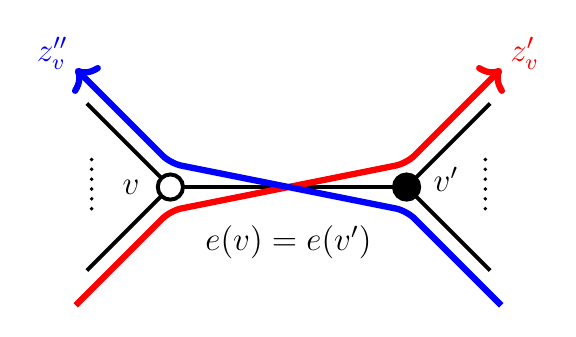
\begin{tikzpicture}
\newcommand{\edgewidth}{0.05cm} %line_width_of _edges
\newcommand{\nodewidth}{0.05cm} %line_width_around_nodes
\newcommand{\noderad}{0.16} %radius_of_node

%coordinate setting
\coordinate (W1) at (0,0); \coordinate (B1) at (3,0);
\path (W1) ++(135:1.5cm) coordinate (W1a); \path (W1) ++(225:1.5cm) coordinate (W1b);
\path (B1) ++(45:1.5cm) coordinate (B1a); \path (B1) ++(315:1.5cm) coordinate (B1b);

%edge
\draw [line width=\edgewidth] (W1)--(B1); \draw [line width=\edgewidth] (W1)--(W1a); \draw [line width=\edgewidth] (W1)--(W1b);
\draw [line width=\edgewidth] (B1)--(B1a); \draw [line width=\edgewidth] (B1)--(B1b);
\draw [line width=\edgewidth,line cap=round, dash pattern=on 0pt off 2.5\pgflinewidth] (-1,0.35)--(-1,-0.35);
\draw [line width=\edgewidth,line cap=round, dash pattern=on 0pt off 2.5\pgflinewidth] (4,0.35)--(4,-0.35);
\draw [line width=\nodewidth, fill=white] (W1) circle [radius=\noderad] ;
\draw [line width=\nodewidth, fill=black] (B1) circle [radius=\noderad] ;

%zigzag
\path (W1) ++(270:0.3cm) coordinate (W1-); \path (W1) ++(90:0.3cm) coordinate (W1+);
\path (B1) ++(270:0.3cm) coordinate (B1-); \path (B1) ++(90:0.3cm) coordinate (B1+);
\path (W1-) ++(225:1.7cm) coordinate (W1--); \path (W1+) ++(135:1.7cm) coordinate (W1++);
\path (B1-) ++(315:1.7cm) coordinate (B1--); \path (B1+) ++(45:1.7cm) coordinate (B1++);
\draw [->, rounded corners, line width=0.08cm, red] (W1--)--(W1-)--(B1+)--(B1++) ;
\draw [->, rounded corners, line width=0.08cm, blue] (B1--)--(B1-)--(W1+)--(W1++) ;

%node
\node at (-0.5,0) {\large$v$} ; \node at (3.5,0.1) {\large$v^\prime$} ;
\node at (1.5,-0.7) {\large$e(v)=e(v^\prime)$} ;
\node[red] at (4.5,1.7) {\large$z_v^\prime$}; \node[blue] at (-1.5,1.7) {\large$z_v^{\prime\prime}$};

\end{tikzpicture}
} }
\end{center}

We then apply the same argument to the node $v^\prime$ which is the other endpoint of $e(v)$.
The proper ordering on $\Gamma$ leads to the conclusion that $e(v)=e(v^\prime)$ (see the above figure).
We repeat these arguments for any node, but it is enough to consider $e(v)$'s for any $v\in\Gamma^+_0$ (or $v\in\Gamma^-_0$).
By \cite[Section~3.2]{Gul} or \cite[Lemma~4.19]{Bro}, we see that the subset of edges $e(v)$ for all $v\in\Gamma^+_0$ forms a perfect matching.
Furthermore, since $z=z_k$ is type I, there exists a zigzag path whose slope is located at an angle less than $\pi$ in an anti-clockwise (resp.\ clockwise) direction from~$[z]$ in~$\xi(v)$ by \cite[Lemma~4.11 and its proof]{Bro}, in which case such a slope is located between $[z]$ and $[z^\prime_v]$ (resp.~$[z^{\prime\prime}_v]$) or coincides with $[z^\prime_v]$ (resp.~$[z^{\prime\prime}_v]$). Thus, we have $z\neq z^\prime_v$ and $z\neq z^{\prime\prime}_v$ by the definition of the ray $\calR$.
Therefore, in this case $e(v)$ is not contained in~$z$ by the above construction.
Also, we see that if a node~$v$ does not lie on~$z$, $e(v)$ is not contained in~$z$.
Thus, the perfect matching constructed in the above fashion satisfies the desired condition.
\end{proof}

\begin{Lemma}\label{lem_same_length}
Let $z$ be a type I zigzag path on a consistent dimer model.
Then, we have $\omega_{\min}(z)=0$, and hence $\ell(z)$ is the same for all type I zigzag paths having the same slope.
\end{Lemma}

\begin{proof}
This follows from Lemmas~\ref{zigzag_lem2} and \ref{lem_existence_pm}.
\end{proof}

For zigzag paths $z$, $w$ on a dimer model $\Gamma$, we denote by $z\cap w$ the subset of edges that are intersections of $z$ and $w$ on $\Gamma$.
We remark that if $z$ is type I then the number of intersections of~$\widetilde{z}$ and~$\widetilde{w}$ on $\widetilde{\Gamma}$ is less than or equal to one, but there are possibly more intersections of~$z$ and~$w$ if we consider them on~$\Gamma$.

\begin{Lemma}\label{intersect_zigorzag}
Let $z$ be a type I zigzag path on a reduced consistent dimer model $\Gamma$.
We suppose that a zigzag path $w$ has intersections with~$z$ on~$\Gamma$.
Then, we see that $z\cap w\subset \Zig(z)$ or $z\cap w\subset \Zag(z)$.
\end{Lemma}

\begin{proof}
Let $e_1$, $e_2$ be edges of $\Gamma$, and we assume that $w$ intersects with $z$ at $e_1$ and~$e_2$.
If~$e_i$ is a~zig of~$z$, then it is a~zag of~$w$, and vice versa. We assume that $e_1$ is a zig of~$z$ and~$e_2$ is a~zag of~$z$.

We then lift these edges on the universal cover $\widetilde{\Gamma}$. Let $\widetilde{e_1}$, $\widetilde{e_2}$ be edges of $\widetilde{\Gamma}$ whose restrictions on $\Gamma$ are $e_1$, $e_2$, respectively. In particular, $\widetilde{e_1}$ is a~zig of~$\widetilde{z}$ and~$\widetilde{e_2}$ is a~zag of~$\widetilde{z}$.
Then, there exist zigzag paths $\widetilde{w}_1$, $\widetilde{w}_2$ on~$\widetilde{\Gamma}$ whose restriction on~$\Gamma$ is just~$w$,
and $\widetilde{w}_1$ (resp.~$\widetilde{w}_2$) intersects with~$\widetilde{z}$ at~$\widetilde{e_1}$ (resp.~$\widetilde{e_2}$).
The zigzag path $\widetilde{z}$ splits $\RR^2$ into two pieces, and~$\widetilde{w}_1$ (resp.~$\widetilde{w}_2$) intersects with~$\widetilde{z}$ from left to right (resp.\ right to left) by the definition of zigzag paths (see the figure below).

\begin{center}
\newcommand{\edgewidth}{0.05cm} %line_width_of _edges
\newcommand{\nodewidth}{0.05cm} %line_width_around_nodes
\newcommand{\noderad}{0.16} %radius_of_node
\scalebox{0.6}{
\begin{tikzpicture}
%coordinate setting
\coordinate (B1) at (1,2); \coordinate (B2) at (3,2); \coordinate (B3) at (3,4);
\coordinate (B4) at (6,2); \coordinate (B5) at (6,4); \coordinate (B6) at (8,2);

\coordinate (W1) at (2,1); \coordinate (W2) at (2,3); \coordinate (W3) at (4,3);
\coordinate (W4) at (7,1); \coordinate (W5) at (7,3);
%edge
\draw [line width=\edgewidth] (2.5,0.5)--(W1)--(B2)--(W2)--(B3)--(2.5,4.5) ;
\draw [line width=\edgewidth,line cap=round, dash pattern=on 0pt off 2.5\pgflinewidth] (2.6,0.4)--(3,0);
\draw [line width=\edgewidth,line cap=round, dash pattern=on 0pt off 2.5\pgflinewidth] (2.4,4.6)--(2,5);
\draw [line width=\edgewidth] (0.5,2.5)--(B1)--(W2)--(B2)--(W3)--(4.5,2.75) ;
\draw [line width=\edgewidth,line cap=round, dash pattern=on 0pt off 2.5\pgflinewidth] (0.4,2.6)--(0,3);
\draw [line width=\edgewidth,line cap=round, dash pattern=on 0pt off 2.5\pgflinewidth] (4.7,2.65)--(5.4,2.3);
\draw [line width=\edgewidth] (5.5,2.25)--(B4)--(W5)--(B6)--(8.5,2.5) ;
\draw [line width=\edgewidth,line cap=round, dash pattern=on 0pt off 2.5\pgflinewidth] (8.6,2.6)--(9,3);
\draw [line width=\edgewidth] (6.5,0.5)--(W4)--(B4)--(W5)--(B5)--(6.5,4.5) ;
\draw [line width=\edgewidth,line cap=round, dash pattern=on 0pt off 2.5\pgflinewidth] (6.4,0.4)--(6,0);
\draw [line width=\edgewidth,line cap=round, dash pattern=on 0pt off 2.5\pgflinewidth] (6.6,4.6)--(7,5);

%blacknode
\draw [line width=\nodewidth, fill=black] (B1) circle [radius=\noderad] ; \draw [line width=\nodewidth, fill=black] (B2) circle [radius=\noderad] ;
\draw [line width=\nodewidth, fill=black] (B3) circle [radius=\noderad] ;
\draw [line width=\nodewidth, fill=black] (B4) circle [radius=\noderad] ; \draw [line width=\nodewidth, fill=black] (B5) circle [radius=\noderad] ;
\draw [line width=\nodewidth, fill=black] (B6) circle [radius=\noderad] ;
%whitenode
\draw [line width=\nodewidth, fill=white] (W1) circle [radius=\noderad] ; \draw [line width=\nodewidth, fill=white] (W2) circle [radius=\noderad] ;
\draw [line width=\nodewidth, fill=white] (W3) circle [radius=\noderad] ;
\draw [line width=\nodewidth, fill=white] (W4) circle [radius=\noderad] ; \draw [line width=\nodewidth, fill=white] (W5) circle [radius=\noderad] ;

%zigzag
\draw [->, rounded corners, line width=0.08cm, blue] (0,3.25)--(1,2.25)--(2,3.25)--(3,2.25)--(4,3.25)--(6,2.25)--(7,3.25)--(8,2.25)--(9,3.25);
\node[blue] at (9.5,3.25) {\Large$\widetilde{z}$} ;
\draw [->, rounded corners, line width=0.08cm, red] (2.75,0)--(1.75,1)--(2.75,2)--(1.75,3)--(2.75,4)--(1.75,5);
\node[red] at (1.75,5.5) {\Large$\widetilde{w}_2$} ;
\draw [<-, rounded corners, line width=0.08cm, red] (6.25,0)--(7.25,1)--(6.25,2)--(7.25,3)--(6.25,4)--(7.25,5);
\node[red] at (6.25,-0.5) {\Large$\widetilde{w}_1$} ;

\node at (4.5,1) {\Large right of $\widetilde{z}$} ; \node at (4.5,4.5) {\Large left of $\widetilde{z}$} ;
\end{tikzpicture}
}
\end{center}

Since $z$ is type I, there is no intersections of $\widetilde{z}$ and $\widetilde{w}_i$ except $\widetilde{e_i}$ where $i=1,2$.
Thus, we can not superimpose $\widetilde{w}_1$ and $\widetilde{w}_2$ using translations.
This contradicts a choice of $\widetilde{w}_1$, $\widetilde{w}_2$.
\end{proof}

The following lemma follows from the argument in the proof of \cite[Proposition~3.12]{Bro}.

\begin{Lemma}\label{slope_linearly_independent}
Let $z$, $w$ be zigzag paths on a consistent dimer model~$\Gamma$.
We assume that $\widetilde{z}$ intersects with $\widetilde{w}$ on the universal cover $\widetilde{\Gamma}$ at most once.
Then, the slopes $[z]$, $[w]$ are linearly independent if and only if~$\widetilde{z}$ and~$\widetilde{w}$ intersect on precisely one edge.
\end{Lemma}

\begin{Lemma}\label{intersect_zigorzag2}
Let $z_1,\dots,z_r$ be type~I zigzag paths on a reduced consistent dimer model $\Gamma$ having the same slope.
We suppose that a zigzag path~$w$ has intersections with $z_j$ for some $j$.
Then, $w$~intersects with every $z_i$ $(i=1,\dots,r)$, and the intersections $w\cap z_1,\dots, w\cap z_r$ are all in $\Zig(w)$ or all in $\Zag(w)$.
Moreover, we have $|w\cap z_1|=\cdots=|w\cap z_r|$.
\end{Lemma}

\begin{proof}
Since $z_1,\dots,z_r$ are type I, $\widetilde{w}$ intersects with each $\widetilde{z_i}$ at most once.
Thus, each pair of zigzag paths $(\widetilde{w},\widetilde{z_i})$ for $i=1,\dots,r$ satisfies the assumption in Lemma~\ref{slope_linearly_independent}.
Since~$w$ has intersections with~$z_j$, $\widetilde{w}$ intersects with $\widetilde{z_j}$ precisely once on the universal cover.
By Lemma~\ref{slope_linearly_independent}, we see that $[w]$ and $[z_j]$ are linearly independent, and hence $[w]$ and $[z_i]$ are linearly independent for any~$i$.
Thus, $\widetilde{w}$ intersects with $\widetilde{z_i}$ precisely once for any $i=1,\dots,r$.

The latter assertion follows from a similar argument as in the proof of Lemma~\ref{intersect_zigorzag}.
More precisely, since $\widetilde{w}$ intersects with $\widetilde{z_i}$ precisely once for any $i=1,\dots,r$,
if $\widetilde{w}$ intersects with $\widetilde{z_i}$ from right to left (resp.\ left to right), then so do zigzag paths having the same slope.
This means that intersections are all in $\Zig(w)$ (resp.\ all in $\Zag(w))$.

Also, let $\widetilde{z_1}$ and $\widetilde{z_1}^\prime$ be zigzag paths on $\widetilde{\Gamma}$ that are projected onto the zigzag path $z_1$ on $\Gamma$.
We assume that there is no zigzag path projected onto $z_1$ between $\widetilde{z_1}$ and $\widetilde{z_1}^\prime$.
Also, we assume that~$\widetilde{w}$ first intersects with~$\widetilde{z_1}$, then intersects with $\widetilde{z_1}^\prime$.
Then, for all $i=2,\dots,r$ we can find a~unique zigzag path~$\widetilde{z_i}$ on $\widetilde{\Gamma}$ such that it is projected onto $z_i$ and is located between~$\widetilde{z_1}$ and~$\widetilde{z_1}^\prime$.
Thus, after $\widetilde{w}$ intersects with $\widetilde{z_1}$, it intersects with $\widetilde{z_2}, \dots, \widetilde{z_r}$ precisely once and then arrives at~$\widetilde{z_1}^\prime$.
We can apply the same arguments for any pair $(\widetilde{z_1},\widetilde{z_1}^\prime)$ of zigzag paths on~$\widetilde{\Gamma}$ satisfying the above properties. Thus, projecting onto~$\Gamma$ we have $|w\cap z_1|=\cdots=|w\cap z_r|$.
\end{proof}


% Original source lines 1274--1527
\section{Deformations of dimer models}\label{sec_def_deform}

In this section, we will introduce the concept of a deformation of consistent dimer models.
This operation is defined for type I zigzag paths on a consistent dimer model, and there are two kinds of deformations,
which we call the zig-deformation (see Definition~\ref{def_deformation_zig}) and the zag-deformation (see Definition~\ref{def_deformation_zag}).
For some special cases, these deformations preserve the consistency condition (see Proposition~\ref{prop_preserve_consistent1}),
but they change the associated PM polygon, whereas we will see that the PM polygon of the deformed dimer model is exactly the combinatorial mutation of a~polygon (see Theorem~\ref{mutation=deformation1}).

\subsection{Definition of deformations of dimer models}\label{subsec_def_deform}

Let $\Gamma$ be a reduced consistent dimer model.
In particular, any slope of a zigzag path on $\Gamma$ is primitive.
Let $\calZ_v(\Gamma)$ be the subset of zigzag paths on $\Gamma$ whose slopes are the primitive vector~$v\in\ZZ^2$,
and $\calZ_v^\rmI(\Gamma)$ be the subset of $\calZ_v(\Gamma)$ consisting of type I zigzag paths.
We first prepare the \emph{deformation data}.

\begin{Definition}[deformation data]\label{def_deformation_data}
Let $\Gamma$ be a reduced consistent dimer model. In order to define the deformation of $\Gamma$, we fix the following data.
\begin{itemize}\itemsep=0pt
\item[(1)] We choose a type I zigzag path $z$, and let $2n\coloneqq\ell(z)$ and $v\coloneqq [z]$.
\item[(2)] We then fix a positive integer $r$ such that $r\le |\calZ_v^\rmI(\Gamma)|$, and let $h=n-r$.
\item[(3)] We take a subset $\{z_1,\dots,z_r\}\subset\calZ_v^\rmI(\Gamma)$ of type I zigzag paths, in which case we have $2n=\ell(z_1)=\cdots=\ell(z_r)$ by Lemma~\ref{lem_same_length}.
Therefore, each $z_i$ can be described as
\begin{displaymath} z_i=z_i[1]z_i[2]\cdots z_i[2n-1]z_i[2n]. \end{displaymath}
\item[(4)]
We consider non-negative integers $p_1,\dots,p_r\in\ZZ_{\ge0}$ such that $p_1+\cdots+p_r=n-r=h$.
We call $\bfp\coloneqq(p_1,\dots,p_r)$ a \emph{deformation weight} of $\{z_1, \dots, z_r\}$.
\end{itemize}
\end{Definition}

\begin{Remark}\label{rem_typeI_to_typeII}
To define the deformation data, we need a type I zigzag path.
If a dimer model is isoradial, then any zigzag path is type I (see Definition~\ref{def_isoradial}), and hence $\big|\calZ_v^\rmI(\Gamma)\big|=|\calZ_v(\Gamma)|$.
Also, even if $\Gamma$ contains no type I zigzag paths, we sometimes change a type II zigzag path into type I by using the \emph{mutations of dimer models}
(see Appendix~\ref{app_mutationdimer}, especially Example~\ref{mutation_typeII_to_I}).
\end{Remark}

\begin{Definition}[zig-deformation]\label{def_deformation_zig}
Let the notation be the same as in Definition~\ref{def_deformation_data}.
For a~deformation weight $\bfp=(p_1,\dots,p_r)$ of $\{z_1, \dots, z_r\}$, we consider the following procedures:
\begin{enumerate}[(\text{zig}-1)]
\setlength{\parskip}{0pt}\itemsep=0pt
\item Using split moves, we insert $p_i$ white nodes and $p_i$ black nodes in each zig of $z_i$.

\noindent{\bf [Notation]}
\begin{itemize}\itemsep=0pt
\item For any zig $z_i[2m-1]$ of $z_i$ where $m=1,\dots,n$ and $i=1,\dots,r$, we denote by $b_i[2m-1]$ (resp.~$w_i[2m-1]$) the black (resp.\ white) node that is the endpoint of $z_i[2m-1]$.
\item We denote the white nodes added in the zig $z_i[2m-1]$ by $w_{i,1}[2m-1],\dots,w_{i,p_i}[2m-1]$, and the black ones by $b_{i,1}[2m-1],\dots,b_{i,p_i}[2m-1]$.
Here, the subscripts increase in the direction from $b_i[2m-1]$ to $w_i[2m-1]$.
\end{itemize}
\item We remove all zags of $z_i$ for every $i=1,\dots,r$.
\item If $p_i\neq 0$, then we connect the white node $w_{i,j}[2m-1]$ to the black node $b_{i,j}[2m+1]$ where $j=1,\dots,p_i$ and $m=1,\dots,n$.
(Note that $w_{i,j}[2n-1]$ is connected to $b_{i,j}[2n+1]\coloneqq b_{i,j}[1]$.)
We denote by $z_{i,j}$ the new $1$-cycle, which will be a zigzag path on the deformed dimer model, obtained by connecting
\begin{displaymath}
w_{i,j}[2n-1], b_{i,j}[2n-1], w_{i,j}[2n-3], b_{i,j}[2n_i-3],\dots,w_{i,j}[1], b_{i,j}[1]
\end{displaymath}
cyclically ($i=1,\dots,r$ and $j=1,\dots,p_i$).
\item[(join)] If there exist $2$-valent nodes, then we apply the join moves to the dimer model obtained by the above procedures and make it reduced.
\end{enumerate}
We denote the resulting dimer model by $\nu^\zig_\bfp(\Gamma, \{z_1,\dots,z_r\})$,
and call it the \emph{zig-deformation of~$\Gamma$ at $\{z_1,\dots,z_r\}$ with respect to the weight $\bfp$}.
If a situation is clear, we simply denote this by~$\nu^\zig_\bfp(\Gamma)$.
\end{Definition}

\begin{figure}[h!]\centering
\scalebox{0.55}{
\begin{tikzpicture}
\newcommand{\edgewidth}{0.05cm} %line_width_of _edges
\newcommand{\nodewidth}{0.05cm} %line_width_around_nodes
\newcommand{\noderad}{0.16} %radius_of_node
%coordinate setting
\coordinate (W1) at (0,1.2); \coordinate (W2) at (0,3.6);
%\coordinate (B1) at (3,0); \coordinate (B2) at (3,2.4);
\path (W1) ++(-20:4cm) coordinate (B1); \path (W2) ++(-20:4cm) coordinate (B2);
\path (B1) ++(200:2cm) coordinate (B0); \path (W2) ++(20:2cm) coordinate (W3);

\path (W1) ++(-20:0.8cm) coordinate (B1-1); \path (W1) ++(-20:1.6cm) coordinate (W1-1);
\path (W1) ++(-20:2.4cm) coordinate (B1-2); \path (W1) ++(-20:3.2cm) coordinate (W1-2);
\path (W2) ++(-20:0.8cm) coordinate (B2-1); \path (W2) ++(-20:1.6cm) coordinate (W2-1);
\path (W2) ++(-20:2.4cm) coordinate (B2-2); \path (W2) ++(-20:3.2cm) coordinate (W2-2);

\path (B1) ++(30:1cm) coordinate (B1e); \path (B1) ++(330:1cm) coordinate (B1s);
\path (W1) ++(150:1cm) coordinate (W1w); \path (W1) ++(210:1cm) coordinate (W1s);
\path (B2) ++(30:1cm) coordinate (B2e); \path (B2) ++(330:1cm) coordinate (B2s);
\path (W2) ++(150:1cm) coordinate (W2w); \path (W2) ++(210:1cm) coordinate (W2s);

\path (W1) ++(160:0.7cm) coordinate (W1+); \path (W1) ++(200:0.7cm) coordinate (W1-);
\path (W2) ++(160:0.7cm) coordinate (W2+); \path (W2) ++(200:0.7cm) coordinate (W2-);
\path (B1) ++(20:0.7cm) coordinate (B1+); \path (B1) ++(340:0.7cm) coordinate (B1-);
\path (B2) ++(20:0.7cm) coordinate (B2+); \path (B2) ++(340:0.7cm) coordinate (B2-);

\node (original) at (0,0) {
\begin{tikzpicture}
%edge
\draw [line width=\edgewidth] (B1)--(W1); \draw [line width=\edgewidth] (B2)--(W1) ; \draw [line width=\edgewidth] (B2)--(W2) ;
\draw [line width=\edgewidth] (B1)--(B0) ; \draw [line width=\edgewidth] (W2)--(W3) ;
\draw [line width=\edgewidth] (B1)--(B1e); \draw [line width=\edgewidth] (B1)--(B1s);
\draw [line width=\edgewidth] (W1)--(W1w); \draw [line width=\edgewidth] (W1)--(W1s);
\draw [line width=\edgewidth] (B2)--(B2e); \draw [line width=\edgewidth] (B2)--(B2s);
\draw [line width=\edgewidth] (W2)--(W2w); \draw [line width=\edgewidth] (W2)--(W2s);

\draw [line width=\edgewidth,line cap=round, dash pattern=on 0pt off 2.5\pgflinewidth] (W1+)--(W1-);
\draw [line width=\edgewidth,line cap=round, dash pattern=on 0pt off 2.5\pgflinewidth] (W2+)--(W2-);
\draw [line width=\edgewidth,line cap=round, dash pattern=on 0pt off 2.5\pgflinewidth] (B1+)--(B1-);
\draw [line width=\edgewidth,line cap=round, dash pattern=on 0pt off 2.5\pgflinewidth] (B2+)--(B2-);
%blacknode
\draw [line width=\nodewidth, fill=black] (B1) circle [radius=\noderad] ; \draw [line width=\nodewidth, fill=black] (B2) circle [radius=\noderad] ;
%whitenode
\draw [line width=\nodewidth, fill=white] (W1) circle [radius=\noderad] ; \draw [line width=\nodewidth, fill=white] (W2) circle [radius=\noderad] ;

%zigzag path
\coordinate (W1z) at (0,1.2); \coordinate (W2z) at (0,3.6);
\path (W1) ++(90:0.2cm) coordinate (W1z); \path (W2) ++(90:0.2cm) coordinate (W2z);
\path (W1z) ++(-20:4cm) coordinate (B1z); \path (W2z) ++(-20:4cm) coordinate (B2z);
\path (B1z) ++(200:2cm) coordinate (B0z); \path (W2z) ++(20:2cm) coordinate (W3z);
\path (B1z) ++(200:2cm) coordinate (B0z); \path (W2z) ++(20:2.2cm) coordinate (W3z);

\path (W1) ++(-90:0.2cm) coordinate (W1zz); \path (W1zz) ++(150:1.5cm) coordinate (W1wzz);
\draw [->, rounded corners, line width=0.08cm, red] (B0z)--(B1z)--(W1z)--(B2z)--(W2z)--(W3z);

\node at (2.5,3.5) {\color{red}\large$z_i[2m+1]$};
\node at (1.2,2.2) {\color{red}\large$z_i[2m]$};
\node at (2.5,1.1) {\color{red}\large$z_i[2m-1]$};
\end{tikzpicture}};

\node (original_insert) at (10,0) {
\begin{tikzpicture}
%edge
\draw [line width=\edgewidth] (B1)--(W1); \draw [line width=\edgewidth] (B2)--(W1) ; \draw [line width=\edgewidth] (B2)--(W2) ;
\draw [line width=\edgewidth] (B1)--(B0) ; \draw [line width=\edgewidth] (W2)--(W3) ;
\draw [line width=\edgewidth] (B1)--(B1e); \draw [line width=\edgewidth] (B1)--(B1s);
\draw [line width=\edgewidth] (W1)--(W1w); \draw [line width=\edgewidth] (W1)--(W1s);
\draw [line width=\edgewidth] (B2)--(B2e); \draw [line width=\edgewidth] (B2)--(B2s);
\draw [line width=\edgewidth] (W2)--(W2w); \draw [line width=\edgewidth] (W2)--(W2s);

\draw [line width=\edgewidth,line cap=round, dash pattern=on 0pt off 2.5\pgflinewidth] (W1+)--(W1-);
\draw [line width=\edgewidth,line cap=round, dash pattern=on 0pt off 2.5\pgflinewidth] (W2+)--(W2-);
\draw [line width=\edgewidth,line cap=round, dash pattern=on 0pt off 2.5\pgflinewidth] (B1+)--(B1-);
\draw [line width=\edgewidth,line cap=round, dash pattern=on 0pt off 2.5\pgflinewidth] (B2+)--(B2-);
%blacknode
\draw [line width=\nodewidth, fill=black] (B1) circle [radius=\noderad] ; \draw [line width=\nodewidth, fill=black] (B2) circle [radius=\noderad] ;
\draw [line width=\nodewidth, fill=black] (B1-1) circle [radius=\noderad] ; \draw [line width=\nodewidth, fill=black] (B1-2) circle [radius=\noderad] ;
\draw [line width=\nodewidth, fill=black] (B2-1) circle [radius=\noderad] ; \draw [line width=\nodewidth, fill=black] (B2-2) circle [radius=\noderad] ;
%whitenode
\draw [line width=\nodewidth, fill=white] (W1) circle [radius=\noderad] ; \draw [line width=\nodewidth, fill=white] (W2) circle [radius=\noderad] ;
\draw [line width=\nodewidth, fill=white] (W1-1) circle [radius=\noderad] ; \draw [line width=\nodewidth, fill=white] (W1-2) circle [radius=\noderad] ;
\draw [line width=\nodewidth, fill=white] (W2-1) circle [radius=\noderad] ; \draw [line width=\nodewidth, fill=white] (W2-2) circle [radius=\noderad] ;
\end{tikzpicture}};


\node (original_remove) at (10,-6.5) {
\begin{tikzpicture}
%edge
\draw [line width=\edgewidth] (B1)--(W1); \draw [line width=\edgewidth] (B2)--(W2);
%\draw [line width=\edgewidth] (B2)--(W1); \draw [line width=\edgewidth] (B1)--(B0); \draw [line width=\edgewidth] (W2)--(W3);
\draw [line width=\edgewidth] (B1)--(B1e); \draw [line width=\edgewidth] (B1)--(B1s);
\draw [line width=\edgewidth] (W1)--(W1w); \draw [line width=\edgewidth] (W1)--(W1s);
\draw [line width=\edgewidth] (B2)--(B2e); \draw [line width=\edgewidth] (B2)--(B2s);
\draw [line width=\edgewidth] (W2)--(W2w); \draw [line width=\edgewidth] (W2)--(W2s);

\draw [line width=\edgewidth,line cap=round, dash pattern=on 0pt off 2.5\pgflinewidth] (W1+)--(W1-);
\draw [line width=\edgewidth,line cap=round, dash pattern=on 0pt off 2.5\pgflinewidth] (W2+)--(W2-);
\draw [line width=\edgewidth,line cap=round, dash pattern=on 0pt off 2.5\pgflinewidth] (B1+)--(B1-);
\draw [line width=\edgewidth,line cap=round, dash pattern=on 0pt off 2.5\pgflinewidth] (B2+)--(B2-);
%blacknode
\draw [line width=\nodewidth, fill=black] (B1) circle [radius=\noderad] ; \draw [line width=\nodewidth, fill=black] (B2) circle [radius=\noderad] ;
\draw [line width=\nodewidth, fill=black] (B1-1) circle [radius=\noderad] ; \draw [line width=\nodewidth, fill=black] (B1-2) circle [radius=\noderad] ;
\draw [line width=\nodewidth, fill=black] (B2-1) circle [radius=\noderad] ; \draw [line width=\nodewidth, fill=black] (B2-2) circle [radius=\noderad] ;
%whitenode
\draw [line width=\nodewidth, fill=white] (W1) circle [radius=\noderad] ; \draw [line width=\nodewidth, fill=white] (W2) circle [radius=\noderad] ;
\draw [line width=\nodewidth, fill=white] (W1-1) circle [radius=\noderad] ; \draw [line width=\nodewidth, fill=white] (W1-2) circle [radius=\noderad] ;
\draw [line width=\nodewidth, fill=white] (W2-1) circle [radius=\noderad] ; \draw [line width=\nodewidth, fill=white] (W2-2) circle [radius=\noderad] ;
\end{tikzpicture}};


\node (before) at (20,-6.5) {
\begin{tikzpicture}
%edge
\draw [line width=\edgewidth] (B1)--(W1); \draw [line width=\edgewidth] (B2)--(W2) ;
\draw [line width=\edgewidth] (B1)--(B1e); \draw [line width=\edgewidth] (B1)--(B1s);
\draw [line width=\edgewidth] (W1)--(W1w); \draw [line width=\edgewidth] (W1)--(W1s);
\draw [line width=\edgewidth] (B2)--(B2e); \draw [line width=\edgewidth] (B2)--(B2s);
\draw [line width=\edgewidth] (W2)--(W2w); \draw [line width=\edgewidth] (W2)--(W2s);

\draw [line width=\edgewidth,line cap=round, dash pattern=on 0pt off 2.5\pgflinewidth] (W1+)--(W1-);
\draw [line width=\edgewidth,line cap=round, dash pattern=on 0pt off 2.5\pgflinewidth] (W2+)--(W2-);
\draw [line width=\edgewidth,line cap=round, dash pattern=on 0pt off 2.5\pgflinewidth] (B1+)--(B1-);
\draw [line width=\edgewidth,line cap=round, dash pattern=on 0pt off 2.5\pgflinewidth] (B2+)--(B2-);

\draw [line width=\edgewidth] (B2-1)--(W1-1); \draw [line width=\edgewidth] (B2-2)--(W1-2);
\path (B1-1) ++(-70:1.5cm) coordinate (B1-1-); \draw [line width=\edgewidth] (B1-1)--(B1-1-);
\path (B1-2) ++(-70:1.5cm) coordinate (B1-2-); \draw [line width=\edgewidth] (B1-2)--(B1-2-);
\path (W2-1) ++(110:1.5cm) coordinate (W2-1-); \draw [line width=\edgewidth] (W2-1)--(W2-1-);
\path (W2-2) ++(110:1.5cm) coordinate (W2-2-); \draw [line width=\edgewidth] (W2-2)--(W2-2-);
%blacknode
\draw [line width=\nodewidth, fill=black] (B1) circle [radius=\noderad] ; \draw [line width=\nodewidth, fill=black] (B2) circle [radius=\noderad] ;
\draw [line width=\nodewidth, fill=black] (B1-1) circle [radius=\noderad] ; \draw [line width=\nodewidth, fill=black] (B1-2) circle [radius=\noderad] ;
\draw [line width=\nodewidth, fill=black] (B2-1) circle [radius=\noderad] ; \draw [line width=\nodewidth, fill=black] (B2-2) circle [radius=\noderad] ;
%whitenode
\draw [line width=\nodewidth, fill=white] (W1) circle [radius=\noderad] ; \draw [line width=\nodewidth, fill=white] (W2) circle [radius=\noderad] ;
\draw [line width=\nodewidth, fill=white] (W1-1) circle [radius=\noderad] ; \draw [line width=\nodewidth, fill=white] (W1-2) circle [radius=\noderad] ;
\draw [line width=\nodewidth, fill=white] (W2-1) circle [radius=\noderad] ; \draw [line width=\nodewidth, fill=white] (W2-2) circle [radius=\noderad] ;
\end{tikzpicture}};

\iffalse
\node (after) at (20,-6.5) {
\begin{tikzpicture}
%edge
\draw [line width=\edgewidth] (B1)--(W1); \draw [line width=\edgewidth] (B2)--(W2) ;
\draw [line width=\edgewidth] (B1)--(B1e); \draw [line width=\edgewidth] (B1)--(B1s);
\draw [line width=\edgewidth] (W1)--(W1w); \draw [line width=\edgewidth] (W1)--(W1s);
\draw [line width=\edgewidth] (B2)--(B2e); \draw [line width=\edgewidth] (B2)--(B2s);
\draw [line width=\edgewidth] (W2)--(W2w); \draw [line width=\edgewidth] (W2)--(W2s);

\draw [line width=\edgewidth,line cap=round, dash pattern=on 0pt off 2.5\pgflinewidth] (W1+)--(W1-);
\draw [line width=\edgewidth,line cap=round, dash pattern=on 0pt off 2.5\pgflinewidth] (W2+)--(W2-);
\draw [line width=\edgewidth,line cap=round, dash pattern=on 0pt off 2.5\pgflinewidth] (B1+)--(B1-);
\draw [line width=\edgewidth,line cap=round, dash pattern=on 0pt off 2.5\pgflinewidth] (B2+)--(B2-);

\draw [line width=\edgewidth] (B2-1)--(W1-1); \draw [line width=\edgewidth] (B2-2)--(W1-2);
\path (B1-1) ++(-70:1.5cm) coordinate (B1-1-); \draw [line width=\edgewidth] (B1-1)--(B1-1-);
\path (B1-2) ++(-70:1.5cm) coordinate (B1-2-); \draw [line width=\edgewidth] (B1-2)--(B1-2-);
\path (W2-1) ++(110:1.5cm) coordinate (W2-1-); \draw [line width=\edgewidth] (W2-1)--(W2-1-);
\path (W2-2) ++(110:1.5cm) coordinate (W2-2-); \draw [line width=\edgewidth] (W2-2)--(W2-2-);

\draw [line width=\edgewidth] (B2-1)--(W1); \draw [line width=\edgewidth] (B2-2)--(W1-1); \draw [line width=\edgewidth] (B2)--(W1-2);
%blacknode
\draw [line width=\nodewidth, fill=black] (B1) circle [radius=\noderad] ; \draw [line width=\nodewidth, fill=black] (B2) circle [radius=\noderad] ;
\draw [line width=\nodewidth, fill=black] (B1-1) circle [radius=\noderad] ; \draw [line width=\nodewidth, fill=black] (B1-2) circle [radius=\noderad] ;
\draw [line width=\nodewidth, fill=black] (B2-1) circle [radius=\noderad] ; \draw [line width=\nodewidth, fill=black] (B2-2) circle [radius=\noderad] ;
%whitenode
\draw [line width=\nodewidth, fill=white] (W1) circle [radius=\noderad] ; \draw [line width=\nodewidth, fill=white] (W2) circle [radius=\noderad] ;
\draw [line width=\nodewidth, fill=white] (W1-1) circle [radius=\noderad] ; \draw [line width=\nodewidth, fill=white] (W1-2) circle [radius=\noderad] ;
\draw [line width=\nodewidth, fill=white] (W2-1) circle [radius=\noderad] ; \draw [line width=\nodewidth, fill=white] (W2-2) circle [radius=\noderad] ;
\end{tikzpicture}};
\fi

\path (original) ++(0:3.5cm) coordinate (original+); \path (original_insert) ++(180:3.5cm) coordinate (original_insert+);
\draw [->, line width=\edgewidth] (original+)--(original_insert+) node[midway,xshift=0cm,yshift=0.5cm] {\LARGE(zig-1)} ;

\path (original_insert) ++(0:3.5cm) coordinate (original_insert-); \path (original_remove) ++(180:3.5cm) coordinate (original_remove+);
\path (original_remove) ++(0:3.5cm) coordinate (original_remove++);
\path (before) ++(180:3.5cm) coordinate (before-); \path (0,-6.5) ++(0:3.5cm) coordinate (before--);

\draw [->, line width=\edgewidth] (before--)--(original_remove+) node[midway,xshift=0cm,yshift=0.5cm] {\LARGE(zig-2)} ;
\draw [->, line width=\edgewidth] (original_remove++)--(before-) node[midway,xshift=0cm,yshift=0.5cm] {\LARGE(zig-3)} ;

%\path (before) ++(0:3.5cm) coordinate (before+); \path (after) ++(180:3.5cm) coordinate (after+);
%\draw [->, line width=\edgewidth] (before+)--(after+) node[midway,xshift=0cm,yshift=0.5cm] {\LARGE(zig-4)} ;
\end{tikzpicture}
}
\caption{The zig-deformation at $z_i$ with $p_i=2$.}\label{fig_zigdeform_p2}
\end{figure}

\setcounter{Theorem}{4}
% Original source lines 1719--1730
\begin{Proposition}\label{prop_preserve_consistent1}
Let the notation be the same as Definitions~{\rm \ref{def_deformation_data}}, {\rm \ref{def_deformation_zig}} and {\rm \ref{def_deformation_zag}}.
We assume that either one of the following conditions is satisfied:
\begin{itemize}\itemsep=0pt
\item[$(i)$] $r=1$ or
\item[$(ii)$] $\Gamma$ is a hexagonal or rectangular dimer model $($see Definition~{\rm \ref{def_hexagonal_square})}.
\end{itemize}
Then, the dimer models $\nu^\zig_\bfp(\Gamma, \{z_1,\dots,z_r\})$ and $\nu^\zag_\bfp(\Gamma, \{z_1,\dots,z_r\})$ are consistent.
\end{Proposition}

\begin{proof}This follows from Proposition~\ref{prop_make_consistent} (see also Remark~\ref{r=1case} and Proposition~\ref{skip_hexagonal_square}).
\end{proof}


% Original source lines 2485--2558
\section{Combinatorial mutations of perfect matching polygons}\label{sec_mutation_polygon1}
In this section, we discuss a relationship between deformations of consistent dimer models and combinatorial mutations of polygons.
We first define combinatorial mutations for lattice polytopes of any dimension, and then we mainly discuss the case of polygons.

\subsection{Preliminaries on combinatorial mutations of polytopes}\label{sec_pre_mutation_polygon}

Following \cite{ACGK}, we introduce combinatorial mutations of polytopes.
Let $N\cong\ZZ^d$ be a lattice of rank $d$, and $P\subset N_\RR\coloneqq N\otimes_\ZZ\RR$ be a convex lattice polytope.
We assume that $P$ contains the origin ${\bf 0}$.
We denote by $\calV(P)$ the set of vertices of $P$.
We say that two polytopes $P,Q\subset N_\RR$ are \emph{isomorphic} if they are transformed into each other by $\GL(d,\ZZ)$-transformations, in which case we denote $P\cong Q$.

We first prepare some notions used in the definition of combinatorial mutations of polytopes.

\begin{Definition}[mutation data]\label{def_mutation_data}
Let $P$ be a convex lattice polytope as above.
In order to define a combinatorial mutation of $P$, we fix the data consisting of a vector $w$ and the associated integers $h_{\max}(P,w)$,
$h_{\min}(P,w)$ and $\width(P,w)$ defined as follows.

Let $w\in M\coloneqq\Hom_\ZZ(N,\ZZ)\cong\ZZ^d$ be a primitive lattice vector.
The element $w\in M$ determines the linear map $\langle w,-\rangle\colon N_\RR\rightarrow \RR$, where $\langle-,- \rangle$ is the natural inner product.
We set
\begin{displaymath}
h_{\max}(P,w)\coloneqq{\max}\{\langle w,u\rangle \,|\, u\in P\} \qquad\text{and}\qquad
h_{\min}(P,w)\coloneqq{\min}\{\langle w,u\rangle \,|\, u\in P\},
\end{displaymath}
which are integers since $P$ is a lattice polytope.
When the situation is clear, we simply denote these by $h_{\max}$ and $h_{\min}$, respectively.
We define the \emph{width} of $P$ with respect to $w$ as
\begin{displaymath}
\width(P,w)\coloneqq h_{\max}(P,w)-h_{\min}(P,w).
\end{displaymath}
\end{Definition}

We note that if the origin ${\bf 0}$ is contained in the strict interior $P^\circ$ of $P$, then $h_{\min}<0$ and $h_{\max}>0$, in which case we have $\width(P,w)\ge2$.
We say that a lattice point $u\in N$ (resp.\ a~subset $F\in N_\RR$) is at \emph{height} $m$ with respect to $w$ if $\langle w,u\rangle=m$
(resp.\ $\langle w,u\rangle=m$ for any $u\in F$).

For each height $h\in\ZZ$, we let
\begin{displaymath}
w_h(P)\coloneqq\operatorname{conv}\{u\in P\cap N \,|\, \langle w,u\rangle=h\},
\end{displaymath}
which is the (possibly empty) convex hull of all lattice points in $P$ at height $h$.
By definition, $w_{h_{\min}}(P)$ and $w_{h_{\max}}(P)$ are faces of $P$.
Using these notions, a combinatorial mutation of $P$ is defined as follows.

\begin{Definition}\label{def_mutation_polygon}
Let the notation be the same as above.
We assume that there exists a lattice polytope $F\subset N_\RR$ such that $\langle w,u\rangle=0$ for any $u\in F$, and
for each negative height $h_{\min}\le h<0$ there exists a possibly empty lattice polytope $G_h\subset N_\RR$ satisfying
\begin{equation}\label{condition_Gh}
\{u\in\calV(P)\,|\, \langle w,u \rangle=h\}\subseteq G_h+(-h)F\subseteq w_h(P),
\end{equation}
where $+$ means the Minkowski sum, and we especially define $Q+\varnothing=\varnothing$ for any polytope $Q$.
We call $F$ a \emph{factor} of $P$ with respect to~$w$.
Then, we define the \emph{combinatorial mutation} of $P$ given by the vector $w$, factor $F$ and polytopes $\{G_h\}$ as
\begin{displaymath}
\mutation_w(P,F)\coloneqq\operatorname{conv}\bigg(\bigcup_{h=h_{\min}}^{-1}G_h\cup\bigcup_{h=0}^{h_{\max}}(w_h(P)+hF)\bigg).
\end{displaymath}
\end{Definition}

We note that the combinatorial mutation is independent of the choice of the polytopes $\{G_h\}$ (see \cite[Proposition~1]{ACGK}).
Also, a translation of the factor $F$ does not affect the combinatorial mutation; that is,
for any $u\in N$ with $\langle w,u\rangle=0$ we have $\mutation_w(P,F)\cong\mutation_w(P,u+F)$; see~\cite{ACGK} for more details.

\begin{Remark}[the combinatorial mutation for the case of $d=2$]\label{rem_def_mutation}
When $d=2$, we choose an edge $E$ of a lattice polygon~$P$, and take $w\in M\cong\ZZ^2$ as a primitive inner normal vector for~$E$.
By the choice of $w$, we see that $w_{h_{\min}}(P)=E$ and $w_{h_{\max}}(P)$ is either a vertex or an edge of~$P$.
Then, we take a primitive lattice element $u_E\in N$ satisfying $\langle w,u_E \rangle=0$, and define the line segment $F\coloneqq\operatorname{conv}\{{\bf 0},u_E\}$,
which is parallel to $E$ at height $0$ and has unit lattice length. Since $u_E$ is uniquely determined up to sign, so is $F$.
In this case, $P$ admits a combinatorial mutation with respect to $w$ (equivalently, there exit polytopes $\{G_h\}$ satisfying (\ref{condition_Gh})) if and only if $|E\cap N|-1\ge -h_{\min}$, see \cite[Lemma~1]{KNP}.
We note that the combinatorial mutation does not depend on the choice of $u_E$ (and hence $F$). That is,
$\mutation_w(P,F)\cong\mutation_w(P,-F)$, which means they are $\GL(2,\ZZ)$-equivalent.
\end{Remark}

\setcounter{Theorem}{4}
% Original source lines 2656--2777
\begin{Proposition}[{see \cite[Lemma~2 and Proposition~2]{ACGK}}]\label{properties_mutation_polygon}
Let the notation be the same as above.
\begin{itemize}\itemsep=0pt
\item[\rm (1)] If $Q\coloneqq\mutation_w(P,F)$, then we have $P=\mutation_{(-w)}(Q,F)$.
\item[\rm (2)] $P$ is a Fano polytope if and only if $\mutation_w(P,F)$ is a Fano polytope.
\end{itemize}
\end{Proposition}

Here, we recall that a convex lattice polytope $P\subset N_\RR$ with $\dim P=d$ is called \emph{Fano} if the origin is contained in the strict interior of $P$,
and the vertices $\calV(P)$ of $P$ are primitive lattice points of $N$.

Then, we consider the combinatorial mutation of a lattice polytope $P$ in terms of the polar dual $P^*$ of $P$ in $M$.
To do this, we must first discuss the polar dual $P^*$ for a polyhedron $P$.
We consider the family of polyhedra (not necessarily convex polytopes) which are of the following form:
\begin{displaymath}
\calP^d \coloneqq \bigg\{ \bigcap_{v \in S} H_{v,\geq -k_v} \cap \bigcap_{v' \in T}H_{v',\geq 0} \subset N_\RR \,|\, S,T \subset M, \; |S|, |T| < \infty, \; k_v \in \ZZ_{>0} \bigg\},
\end{displaymath}
where $H_{v,\geq k}=\{u \in N_\RR \,|\, \langle v,u \rangle \geq k\}$ for $v \in M$ and $k \in \RR$.
We note that any lattice polytope containing the origin of~$N_\RR$ belongs to $\calP^d$ but the ones not containing the origin do not belong to~$\calP^d$
since one of the supporting hyperplanes of such a polytope is of the form $H_{v, \geq k}$ for some $v \in M$ and some positive integer~$k$.
Similarly, we define~$\calQ^d$ by swapping the roles of~$N_\RR$ and~$M_\RR$.

For a given $P \in \calP^d$, we consider the \emph{polar dual} $P^* \subset M_\RR$ of $P$ defined as
\begin{displaymath}
P^* \coloneqq \{v \in M_\RR\,|\,\langle v,u\rangle\ge-1 \text{ for all } u\in P\}\subset M_\RR.
\end{displaymath}
Then, we have the following statements.

\begin{Proposition}\label{prop_dual_polytope}
Let the notation be the same as above. Then, for any $P \in \calP^d$ we have
\begin{itemize}\itemsep=0pt
\item[$(i)$] $P^* \in \calQ^d$,
\item[$(ii)$] $(P^*)^*=P$.
\end{itemize}
\end{Proposition}

\begin{proof}(i) Let $P \in \calP^d$. Since $P$ is a polyhedron, there exist a polytope~$Q$ and a polyhedral cone~$C$ such that
$P=Q+C$, where $+$ denotes the Minkowski sum (see \cite[Corollary~7.1b]{Sch}).
Let $Q=\operatorname{conv}\big(\big\{\frac{1}{k_1}u_1,\dots,\frac{1}{k_p}u_p\big\}\big)$ and let $C=\operatorname{cone}(\{u_1',\dots,u_q'\})$.
Note that we can choose~$u_i$,~$u_j'$ from $N$ and $k_i \in \ZZ_{>0}$ because of the form of~$P$.
In what follows, we will show that
\begin{displaymath}
P^*=\bigcap_{i=1}^p H_{u_i,\geq -k_i} \cap \bigcap_{j=1}^qH_{u_j',\geq 0}.
\end{displaymath}

First, we take $v \in P^*$. Then, we have $\langle v,u \rangle \geq -1$ for any $u \in P$.
Since $\frac{1}{k_i}u_i \in Q+{\bf 0} \subset P$, where ${\bf 0} \in C$ denotes the origin,
we see that $\langle v, \frac{1}{k_i}u_i \rangle \geq -1$, i.e., $\langle v, u_i \rangle \geq -k_i$ for each $i$.
If there is $j$ with $\langle v,u_j' \rangle<0$, then $\langle v, u'+ru_j' \rangle < -1$ for some $u' \in Q$ and some sufficiently large~$r$.
Moreover, we have $u'+ru_j' \in Q+C=P$. This contradicts $v \in P^*$; thus $\langle v,u_j' \rangle\geq 0$ for each~$j$.
Therefore, $v \in \bigcap_{i=1}^p H_{u_i,\geq -k_i} \cap \bigcap_{j=1}^qH_{u_j',\geq 0}$.

On the other hand, we take $v \in \bigcap_{i=1}^p H_{u_i,\geq -k_i} \cap \bigcap_{j=1}^qH_{u_j',\geq 0}$.
For any $u \in P$, as mentioned above, there exist $u' \in Q$ and $u'' \in C$ such that $u=u'+u''$.
Let $u'=\sum_{i=1}^p \frac{r_i}{k_i}u_i$, where $r_i \geq 0$ with $\sum_{i=1}^pr_i=1$, and let $u''=\sum_{j=1}^q s_ju_j'$, where $s_j \geq 0$.
By using these expressions together with the inequalities $\langle v,u_i \rangle \geq -k_i$ for each $i$ and $\langle v,u_j' \rangle \geq 0$ for each $j$, we see that
\begin{align*}
\langle v,u \rangle = \langle v,u' \rangle+\langle v,u'' \rangle =
\sum_{i=1}^p \frac{r_i}{k_i}\langle v,u_i \rangle+\sum_{j=1}^q s_j\langle v,u_j' \rangle \geq -\sum_{i=1}^pr_i=-1,
\end{align*}
and thus we have $v \in P^*$.

(ii) For any $u \in P$, we have $\langle v,u\rangle\geq -1$ for any $v \in P^*$, which means that $P \subset (P^*)^*$.
For the other inclusion, we take $u \in N_\RR \setminus P$.
Let $P=\bigcap_{v \in S} H_{v,\geq -k_v} \cap \bigcap_{v' \in T}H_{v',\geq 0}$.
Then either $\langle v,u \rangle <-k_v$ for some $v \in S$ or $\langle v',u \rangle < 0$ for some $v' \in T$ holds.
In the former case, since $\langle v,u' \rangle \geq -k_v$ for any $u' \in P$, we have $\frac{1}{k_v}v \in P^*$.
This means that there is $v''\coloneqq\frac{1}{k_v}v \in P^*$ such that $\langle v'',u \rangle<-1$, and hence $u \not\in (P^*)^*$.
Similarly, in the latter case, since $\langle rv',u' \rangle \geq 0 \geq -1$ for any $u' \in P$ and $r \geq 0$, we have $rv' \in P^*$.
This implies that $u \not\in (P^*)^*$ for sufficiently large $r$, and hence $u \not\in (P^*)^*$. Therefore, we obtain $(P^*)^* \subset P$, as required.
\end{proof}

We next define a map
\[
\varphi_{w,F}\colon \ M_\RR\rightarrow M_\RR \qquad \text{as} \quad \varphi_{w,F}(v)\coloneqq v-v_{\min}w,
\]
where \mbox{$v_{\min}\coloneqq {\min}\{\langle v, u\rangle\,|\, u\in F\}$}.
In particular, when $d=2$ (see Remark~\ref{rem_def_mutation}), this map can be described as
\begin{equation}\label{mutation_M}
\varphi_{w,F}(v)=
\begin{cases}
v & \text{if $\langle v,u_E\rangle\ge0$}, \\
v-\langle v,u_E\rangle w&\text{if $\langle v,u_E\rangle<0$},
\end{cases}
\end{equation}
with $F=\operatorname{conv}\{{\bf 0},u_E\}$.
The next proposition is crucial to prove our main result Theorem~\ref{mutation=deformation}.


\begin{Proposition}
\label{prop_mutation_dual_polytope}
For any $P \in \calP^d$, we have
\begin{displaymath}\varphi_{w,F}(P^*)=\mut_w(P,F)^*.
\end{displaymath}
\end{Proposition}

\begin{proof}
Although this equality essentially follows from \cite[Proposition~4]{ACGK} and the discussions in \cite[p.~12]{ACGK}, we give a precise proof for completeness.

Let $\varphi=\varphi_{w,F}$ and $Q=\mut_w(P,F)$.
To show $\varphi(P^*)\subset Q^*$, we take $v \in P^*$ arbitrarily and consider $\varphi(v)=v - v_{\min}w \in \varphi(P^*)$.
We will show that $\langle v - v_{\min}w,u \rangle \geq -1$ for any $u \in Q$.
It suffices to show this for each vertex $u\in\calV(Q)$.
\begin{itemize}\itemsep=0pt
\item Let $u\in\calV(Q)$ with $\langle w,u \rangle \geq 0$. Then we can write $u=u_P+\langle w,u_P \rangle u_F$ for some $u_P \in \calV(P)$ and $u_F \in \calV(F)$.
In particular, we have
\begin{displaymath}
\langle v-v_{\min}w, u\rangle = \langle v,u_P \rangle + \langle w,u_P \rangle(\langle v,u_F \rangle-v_{\min}) \geq \langle v,u_P \rangle \geq -1.
\end{displaymath}

\item Let $u\in\calV(Q)$ with $\langle w,u \rangle < 0$. For any $u_F \in \calV(F)$, we have $u-\langle w,u \rangle u_F \in P$.
Hence, $\langle v,u-\langle w,u \rangle u_F \rangle \geq -1$. In particular, $\langle v,u \rangle \geq -1 + v_{\min} \langle w,u \rangle$. Thus, we see that
\begin{displaymath}
\langle v-v_{\min}w, u\rangle =\langle v, u\rangle - v_{\min} \langle w, u\rangle \geq -1.
\end{displaymath}
\end{itemize}

To show $Q^*\subset\varphi(P^*)$, we will show that for any $v \in Q^*$ there is $v' \in P^*$ such that $v=\varphi(v')$.
Let $\Delta_F$ be the normal fan of $F$ in $M_\RR$ and let $\sigma \in \Delta_F$ be a maximal cone in $\Delta_F$.
The discussions in \cite[p.~12]{ACGK} say that there exists $M_\sigma \in \GL_d(\ZZ)$ such that the map $\varphi$ is equal to $M_\sigma$,
i.e., $\varphi(v)=vM_\sigma$. Thus, we conclude that $\varphi(v')=v$ for $v'=vM_\sigma^{-1}$.
\end{proof}

\setcounter{Theorem}{9}
% Original source lines 3310--3324
\begin{Theorem}\label{mutation=deformation1}
Let the notation be the same as in Definitions {\rm \ref{def_deformation_data}}, {\rm \ref{def_deformation_zig}} and {\rm \ref{def_deformation_zag}}.
We assume that either one of the following conditions is satisfied:
\begin{itemize}\itemsep=0pt
\item[$(i)$] $r=1$ or
\item[$(ii)$] $\Gamma$ is a hexagonal or rectangular dimer model $($see Definition~{\rm \ref{def_hexagonal_square})}.
\end{itemize}
Then we have
\begin{gather*}
\mutation_{w}(\Delta_\Gamma,F)=\Delta_{\nu^\zig_\bfp(\Gamma,\{z_1,\dots,z_r\})},
\\
\mutation_{w}(\Delta_\Gamma,-F)=\Delta_{\nu^\zag_\bfp(\Gamma,\{z_1,\dots,z_r\})}
\end{gather*}
for certain choices of the deformation data and the mutation data $($see Setting~{\rm \ref{mutation_deformation_setting})}.
\end{Theorem}


% Original source lines 3338--3556
\section{Extended deformations of dimer models}\label{sec_def_exdeform}

In this section, we add some procedures to the deformations given in Definitions~\ref{def_deformation_zig} and \ref{def_deformation_zag}
to construct a consistent dimer model having the same properties as Theorem~\ref{mutation=deformation1} in a more general situation.
The operations which will be introduced in this section might be complicated, thus we refer the reader to Figures~\ref{def_leftright}--\ref{fig_observation_zigzag4}
in the next section and Appendix~\ref{app_large_example} for recognizing their points.

\begin{setting}\label{def_deformation_exdata}
Let $\Gamma$ be a reduced consistent dimer model.
As in Definition~\ref{def_deformation_data}, we choose a~type~I zigzag path $z$, and we let $2n\coloneqq\ell(z)$ and $v\coloneqq [z]$.
We fix positive integers $r, h$ such that $r\le \big|\calZ_v^\rmI(\Gamma)\big|$ and $n=r+h$,
and take a subset $\{z_1,\dots,z_r\}\subset\calZ_v^\rmI(\Gamma)$ of type I zigzag paths.
We recall that we have $2n=\ell(z_1)=\cdots=\ell(z_r)$ by Lemma~\ref{lem_same_length}, and hence we write $z_i$ as
\begin{displaymath}
z_i=z_i[1]z_i[2]\cdots z_i[2n-1]z_i[2n].
\end{displaymath}

Then we prepare the additional data as follows.
\begin{itemize}\itemsep=0pt
\item[(1)] We consider all zigzag paths $x_1,\dots, x_s$ (resp.~$y_1,\dots, y_t$) intersecting with $z$ at some zags (resp.\ zigs) of $z$.
In this case, each of $x_1,\dots, x_s$ (resp.\ $y_1,\dots, y_t$) intersects with any $z_i$ at some zags (resp.\ zigs) of $z_i$ for all $i=1,\dots,r$ by Lemma~\ref{intersect_zigorzag2}.
We may assume that $z_1,\dots,z_r$ are ordered cyclically in the sense that if $x_j$ (resp.~$y_k$) intersects with $z_i$,
then it also intersects with $z_{i-1}$ (resp.~$z_{i+1}$).
\item[(2)]
We recall that $|x_j\cap z_i|$ (resp.~$|y_k\cap z_i|$) is the same number for any $i=1,\dots,r$ by Lemma~\ref{intersect_zigorzag2}.
Thus, for $j\in\{1,\dots, s\}$ let $m_j\coloneqq|x_j\cap z_i|$ be this constant, and for $k\in\{1,\dots, t\}$ let $m^\prime_k\coloneqq|y_k\cap z_i|$.
We note that $n=m_1+\cdots+m_s=m^\prime_1+\cdots+m^\prime_t$.
\item[(3)] Then, we divide each zigzag path $x_j$ into $m_j$ parts $x_j^{(1)},\dots,x_j^{(m_j)}$ as follows.
We first fix one of the intersections of $z_r$ and $x_j$ as the starting edge of $x_j^{(1)}$,
and tracing along $x_j$ we will arrive at another intersection of~$z_r$ and~$x_j$.
We consider the edge of $x_j$ just before this intersection as the ending edge of $x_j^{(1)}$, and consider the second intersection as the starting edge of $x_j^{(2)}$.
Repeating this procedure, we obtain $x_j^{(1)},\dots,x_j^{(m_j)}$ and the set of sub-zigzag paths:
\begin{equation}\label{subzigzag_x}
\big\{x_1^{(1)},\dots,x_1^{(m_1)}, x_2^{(1)},\dots,x_2^{(m_2)}, \dots, x_s^{(1)},\dots,x_s^{(m_s)}\big\}.
\end{equation}

Similarly, we also divide each zigzag path $y_k$ into $m^\prime_k$ parts $y_k^{(1)},\dots,y_k^{(m^\prime_k)}$
by considering one of the intersections of $z_1$ and $y_k$ as the starting edge of $y_k^{(1)}$, and obtain the set of sub-zigzag paths:
\begin{equation}\label{subzigzag_y}
\big\{y_1^{(1)},\dots,y_1^{(m^\prime_1)}, y_2^{(1)},\dots,y_2^{(m^\prime_2)}, \dots, y_t^{(1)},\dots,y_t^{(m^\prime_t)}\big\}.
\end{equation}
\item[(4)]
We then assign one of $\{z_1, \dots, z_r\}$ to $x_j^{(a_j)}$ for $j=1, \dots, s$ and $a_j=1, \dots, m_j$.
Then, we define $X_i$ as the set of edges consisting of the intersections between $z_i$ and the sub-zigzag paths in~(\ref{subzigzag_x}) that are assigned with~$z_i$.
We can make this assignment so that $|X_i|\ge1$, and then set $p_i\coloneqq|X_i|-1$ for $i=1,\dots,r$.
We call $\calX\coloneqq\{X_1,\dots,X_r\}$ a \emph{zig-deformation parameter} with respect to $z_1,\dots,z_r$ and call the tuple $\bfp=(p_1,\dots,p_r)\in\ZZ^r_{\ge0}$ the \emph{weight} of $\calX$.
Similarly, we assign one of $\{z_1, \dots, z_r\}$ to $y_k^{(b_k)}$ for $k=1, \dots, t$ and $b_k=1, \dots, m^\prime_k$.
Then, we define $Y_i$ as the set of edges consisting of the intersections between $z_i$ and the sub-zigzag paths in~(\ref{subzigzag_y}) that are assigned with~$z_i$.
We can make this assignment so that $|Y_i|\ge1$, and then set $q_i\coloneqq|Y_i|-1$ for $i=1,\dots,r$.
We call $\calY\coloneqq\{Y_1,\dots,Y_r\}$ a \emph{zag-deformation parameter} with respect to $z_1,\dots,z_r$ and call the tuple $\bfq=(q_1,\dots,q_r)\in\ZZ^r_{\ge0}$ the \emph{weight} of $\calY$.
We remark that $p_1+\cdots+p_r=m_1+\cdots+m_s-r=n-r=h$, and also that $q_1+\cdots+q_r=h$.
\end{itemize}
\end{setting}

\begin{Definition}[extended zig-deformation]\label{def_exdeformation_zig}
Let the notation be the same as in Setting~\ref{def_deformation_exdata}.
For a zig-deformation parameter $\calX=\{X_1,\dots,X_r\}$ of weight $\bfp=(p_1,\dots,p_r)$, we consider
the operations (zig-1), (zig-2), (zig-3) defined in Definition~\ref{def_deformation_zig} and use the same notation.
Then we conduct the following procedures:
\begin{itemize}\itemsep=0pt
\setlength{\parskip}{0pt}
\setlength{\leftskip}{0.3cm}
\item[(\text{zig}-4)]
For $m=1,\dots,n$ and $i=1, \dots, r$, if the zag $z_i[2m]$ of the original zigzag path~$z_i$ on~$\Gamma$ is not contained in~$X_i$,
then we add edges, which we call \emph{bypasses}
(since these edges provide a new route that connect edges of the zigzag path $x_j$ contained in non-deformed parts, see Figure~\ref{fig_observation_zigzag4}),
connecting the following pairs of black and white nodes:
\begin{align*}
(w_{i,1}[2m-1], &\, b_i[2m+1]), \,(w_{i,2}[2m-1],b_{i,1}[2m+1]), \\ &\dots, (w_{i,p_i}[2m-1],b_{i,p_i-1}[2m+1]),\, (w_i[2m-1],b_{i,p_i}[2m+1]).
\end{align*}
We denote the resulting dimer mode by $\overline{\nu}^\zig_\calX(\Gamma, \{z_1,\dots,z_r\})$.

We note that $\overline{\nu}^\zig_\calX(\Gamma, \{z_1,\dots,z_r\})$ is non-degenerate by Proposition~\ref{prop_nondegenerate}.
\item[(\text{zig}-5)]
Then, we make the dimer model $\overline{\nu}^\zig_\calX(\Gamma, \{z_1,\dots,z_r\})$ consistent using the method given in the proof of \cite[Theorem~1.1]{BIU} (see Operation~\ref{operation_BIU} and Proposition~\ref{prop_make_consistent}).
\end{itemize}

At the end, we perform the operation (join) if the resulting dimer model contains $2$-valent nodes.
We denote the resulting dimer model by $\nu^\zig_\calX(\Gamma, \{z_1,\dots,z_r\})$,
and call it the \emph{extended zig-deformation of $\Gamma$ at $\{z_1,\dots,z_r\}$ with respect to the zig-deformation parameter $\calX$}.
If the situation is clear, we simply denote this by $\nu^\zig_\calX(\Gamma)$.
\end{Definition}

\begin{figure}[h!]\centering\vspace*{-10mm}
\scalebox{0.55}{
\begin{tikzpicture}
\newcommand{\edgewidth}{0.05cm} %line_width_of _edges
\newcommand{\nodewidth}{0.05cm} %line_width_around_nodes
\newcommand{\noderad}{0.16} %radius_of_node
%coordinate setting
\coordinate (W1) at (0,1.2); \coordinate (W2) at (0,3.6);
%\coordinate (B1) at (3,0); \coordinate (B2) at (3,2.4);
\path (W1) ++(-20:4cm) coordinate (B1); \path (W2) ++(-20:4cm) coordinate (B2);
\path (B1) ++(200:2cm) coordinate (B0); \path (W2) ++(20:2cm) coordinate (W3);

\path (W1) ++(-20:0.8cm) coordinate (B1-1); \path (W1) ++(-20:1.6cm) coordinate (W1-1);
\path (W1) ++(-20:2.4cm) coordinate (B1-2); \path (W1) ++(-20:3.2cm) coordinate (W1-2);
\path (W2) ++(-20:0.8cm) coordinate (B2-1); \path (W2) ++(-20:1.6cm) coordinate (W2-1);
\path (W2) ++(-20:2.4cm) coordinate (B2-2); \path (W2) ++(-20:3.2cm) coordinate (W2-2);

\path (B1) ++(30:1cm) coordinate (B1e); \path (B1) ++(330:1cm) coordinate (B1s);
\path (W1) ++(150:1cm) coordinate (W1w); \path (W1) ++(210:1cm) coordinate (W1s);
\path (B2) ++(30:1cm) coordinate (B2e); \path (B2) ++(330:1cm) coordinate (B2s);
\path (W2) ++(150:1cm) coordinate (W2w); \path (W2) ++(210:1cm) coordinate (W2s);

\path (W1) ++(160:0.7cm) coordinate (W1+); \path (W1) ++(200:0.7cm) coordinate (W1-);
\path (W2) ++(160:0.7cm) coordinate (W2+); \path (W2) ++(200:0.7cm) coordinate (W2-);
\path (B1) ++(20:0.7cm) coordinate (B1+); \path (B1) ++(340:0.7cm) coordinate (B1-);
\path (B2) ++(20:0.7cm) coordinate (B2+); \path (B2) ++(340:0.7cm) coordinate (B2-);

\node (original) at (0,0) {
\begin{tikzpicture}
%edge
\draw [line width=\edgewidth] (B1)--(W1); \draw [line width=\edgewidth] (B2)--(W1) ; \draw [line width=\edgewidth] (B2)--(W2) ;
\draw [line width=\edgewidth] (B1)--(B0) ; \draw [line width=\edgewidth] (W2)--(W3) ;
\draw [line width=\edgewidth] (B1)--(B1e); \draw [line width=\edgewidth] (B1)--(B1s);
\draw [line width=\edgewidth] (W1)--(W1w); \draw [line width=\edgewidth] (W1)--(W1s);
\draw [line width=\edgewidth] (B2)--(B2e); \draw [line width=\edgewidth] (B2)--(B2s);
\draw [line width=\edgewidth] (W2)--(W2w); \draw [line width=\edgewidth] (W2)--(W2s);

\draw [line width=\edgewidth,line cap=round, dash pattern=on 0pt off 2.5\pgflinewidth] (W1+)--(W1-);
\draw [line width=\edgewidth,line cap=round, dash pattern=on 0pt off 2.5\pgflinewidth] (W2+)--(W2-);
\draw [line width=\edgewidth,line cap=round, dash pattern=on 0pt off 2.5\pgflinewidth] (B1+)--(B1-);
\draw [line width=\edgewidth,line cap=round, dash pattern=on 0pt off 2.5\pgflinewidth] (B2+)--(B2-);
%blacknode
\draw [line width=\nodewidth, fill=black] (B1) circle [radius=\noderad] ; \draw [line width=\nodewidth, fill=black] (B2) circle [radius=\noderad] ;
%whitenode
\draw [line width=\nodewidth, fill=white] (W1) circle [radius=\noderad] ; \draw [line width=\nodewidth, fill=white] (W2) circle [radius=\noderad] ;

%zigzag path
\coordinate (W1z) at (0,1.2); \coordinate (W2z) at (0,3.6);
\path (W1) ++(90:0.2cm) coordinate (W1z); \path (W2) ++(90:0.2cm) coordinate (W2z);
\path (W1z) ++(-20:4cm) coordinate (B1z); \path (W2z) ++(-20:4cm) coordinate (B2z);
\path (B1z) ++(200:2cm) coordinate (B0z); \path (W2z) ++(20:2cm) coordinate (W3z);
\path (B1z) ++(200:2cm) coordinate (B0z); \path (W2z) ++(20:2.2cm) coordinate (W3z);

\path (B2) ++(-90:0.2cm) coordinate (B2zz); \path (B2zz) ++(330:1cm) coordinate (B2szz);
\path (W1) ++(-90:0.2cm) coordinate (W1zz); \path (W1zz) ++(150:1.5cm) coordinate (W1wzz);

\draw [->, rounded corners, line width=0.08cm, blue] (B2szz)--(B2zz)--(W1zz)--(W1wzz);
\draw [->, rounded corners, line width=0.08cm, red] (B0z)--(B1z)--(W1z)--(B2z)--(W2z)--(W3z);

\node at (2.5,3.5) {\color{red}\large$z_i[2m+1]$};
\node at (1.2,2.2) {\color{red}\large$z_i[2m]$};
\node at (2.5,1.1) {\color{red}\large$z_i[2m-1]$};
\node at (-1.2,2.2) {\color{blue}\large$x_j$};
\end{tikzpicture}};

\node (before) at (10,0) {
\begin{tikzpicture}
%edge
\draw [line width=\edgewidth] (B1)--(W1); \draw [line width=\edgewidth] (B2)--(W2) ;
\draw [line width=\edgewidth] (B1)--(B1e); \draw [line width=\edgewidth] (B1)--(B1s);
\draw [line width=\edgewidth] (W1)--(W1w); \draw [line width=\edgewidth] (W1)--(W1s);
\draw [line width=\edgewidth] (B2)--(B2e); \draw [line width=\edgewidth] (B2)--(B2s);
\draw [line width=\edgewidth] (W2)--(W2w); \draw [line width=\edgewidth] (W2)--(W2s);

\draw [line width=\edgewidth,line cap=round, dash pattern=on 0pt off 2.5\pgflinewidth] (W1+)--(W1-);
\draw [line width=\edgewidth,line cap=round, dash pattern=on 0pt off 2.5\pgflinewidth] (W2+)--(W2-);
\draw [line width=\edgewidth,line cap=round, dash pattern=on 0pt off 2.5\pgflinewidth] (B1+)--(B1-);
\draw [line width=\edgewidth,line cap=round, dash pattern=on 0pt off 2.5\pgflinewidth] (B2+)--(B2-);

\draw [line width=\edgewidth] (B2-1)--(W1-1); \draw [line width=\edgewidth] (B2-2)--(W1-2);
\path (B1-1) ++(-70:1.5cm) coordinate (B1-1-); \draw [line width=\edgewidth] (B1-1)--(B1-1-);
\path (B1-2) ++(-70:1.5cm) coordinate (B1-2-); \draw [line width=\edgewidth] (B1-2)--(B1-2-);
\path (W2-1) ++(110:1.5cm) coordinate (W2-1-); \draw [line width=\edgewidth] (W2-1)--(W2-1-);
\path (W2-2) ++(110:1.5cm) coordinate (W2-2-); \draw [line width=\edgewidth] (W2-2)--(W2-2-);
%blacknode
\draw [line width=\nodewidth, fill=black] (B1) circle [radius=\noderad] ; \draw [line width=\nodewidth, fill=black] (B2) circle [radius=\noderad] ;
\draw [line width=\nodewidth, fill=black] (B1-1) circle [radius=\noderad] ; \draw [line width=\nodewidth, fill=black] (B1-2) circle [radius=\noderad] ;
\draw [line width=\nodewidth, fill=black] (B2-1) circle [radius=\noderad] ; \draw [line width=\nodewidth, fill=black] (B2-2) circle [radius=\noderad] ;
%whitenode
\draw [line width=\nodewidth, fill=white] (W1) circle [radius=\noderad] ; \draw [line width=\nodewidth, fill=white] (W2) circle [radius=\noderad] ;
\draw [line width=\nodewidth, fill=white] (W1-1) circle [radius=\noderad] ; \draw [line width=\nodewidth, fill=white] (W1-2) circle [radius=\noderad] ;
\draw [line width=\nodewidth, fill=white] (W2-1) circle [radius=\noderad] ; \draw [line width=\nodewidth, fill=white] (W2-2) circle [radius=\noderad] ;
\end{tikzpicture}};

\node (after) at (20,0) {
\begin{tikzpicture}
%edge
\draw [line width=\edgewidth] (B1)--(W1); \draw [line width=\edgewidth] (B2)--(W2) ;
\draw [line width=\edgewidth] (B1)--(B1e); \draw [line width=\edgewidth] (B1)--(B1s);
\draw [line width=\edgewidth] (W1)--(W1w); \draw [line width=\edgewidth] (W1)--(W1s);
\draw [line width=\edgewidth] (B2)--(B2e); \draw [line width=\edgewidth] (B2)--(B2s);
\draw [line width=\edgewidth] (W2)--(W2w); \draw [line width=\edgewidth] (W2)--(W2s);

\draw [line width=\edgewidth,line cap=round, dash pattern=on 0pt off 2.5\pgflinewidth] (W1+)--(W1-);
\draw [line width=\edgewidth,line cap=round, dash pattern=on 0pt off 2.5\pgflinewidth] (W2+)--(W2-);
\draw [line width=\edgewidth,line cap=round, dash pattern=on 0pt off 2.5\pgflinewidth] (B1+)--(B1-);
\draw [line width=\edgewidth,line cap=round, dash pattern=on 0pt off 2.5\pgflinewidth] (B2+)--(B2-);

\draw [line width=\edgewidth] (B2-1)--(W1-1); \draw [line width=\edgewidth] (B2-2)--(W1-2);
\path (B1-1) ++(-70:1.5cm) coordinate (B1-1-); \draw [line width=\edgewidth] (B1-1)--(B1-1-);
\path (B1-2) ++(-70:1.5cm) coordinate (B1-2-); \draw [line width=\edgewidth] (B1-2)--(B1-2-);
\path (W2-1) ++(110:1.5cm) coordinate (W2-1-); \draw [line width=\edgewidth] (W2-1)--(W2-1-);
\path (W2-2) ++(110:1.5cm) coordinate (W2-2-); \draw [line width=\edgewidth] (W2-2)--(W2-2-);

\draw [line width=\edgewidth] (B2-1)--(W1); \draw [line width=\edgewidth] (B2-2)--(W1-1); \draw [line width=\edgewidth] (B2)--(W1-2);
%blacknode
\draw [line width=\nodewidth, fill=black] (B1) circle [radius=\noderad] ; \draw [line width=\nodewidth, fill=black] (B2) circle [radius=\noderad] ;
\draw [line width=\nodewidth, fill=black] (B1-1) circle [radius=\noderad] ; \draw [line width=\nodewidth, fill=black] (B1-2) circle [radius=\noderad] ;
\draw [line width=\nodewidth, fill=black] (B2-1) circle [radius=\noderad] ; \draw [line width=\nodewidth, fill=black] (B2-2) circle [radius=\noderad] ;
%whitenode
\draw [line width=\nodewidth, fill=white] (W1) circle [radius=\noderad] ; \draw [line width=\nodewidth, fill=white] (W2) circle [radius=\noderad] ;
\draw [line width=\nodewidth, fill=white] (W1-1) circle [radius=\noderad] ; \draw [line width=\nodewidth, fill=white] (W1-2) circle [radius=\noderad] ;
\draw [line width=\nodewidth, fill=white] (W2-1) circle [radius=\noderad] ; \draw [line width=\nodewidth, fill=white] (W2-2) circle [radius=\noderad] ;
\end{tikzpicture}};

\path (original) ++(0:3.5cm) coordinate (original+); \path (before) ++(180:3.5cm) coordinate (before+);
\draw [->, line width=\edgewidth] (original+)--(before+) node[midway,xshift=-0.5cm,yshift=1.2cm] {\LARGE(zig-1)}
node[midway,xshift=0.5cm,yshift=0.5cm] {\LARGE--\,(zig-3)};

\path (before) ++(0:3.5cm) coordinate (before-); \path (after) ++(180:3.5cm) coordinate (after+);
\draw [->, line width=\edgewidth] (before-)--(after+) node[midway,xshift=0cm,yshift=0.5cm] {\LARGE(zig-4)} ;

\end{tikzpicture}
}
\caption{The operations (zig-1)--(zig-4) at $z_i$ for the case $p_i=|X_i|-1=2$ and $z_i[m]\not\in X_i$.}\label{fig_exzigdeform_p2}
\end{figure}

\setcounter{Theorem}{3}
% Original source lines 3725--3737
\begin{Remark}\label{r=1case}
If $r=1$, then we consider deformation parameters $\calX=\{X_1\}$ and $\calY=\{Y_1\}$ in Setting~\ref{def_deformation_exdata},
where~$X_1$ (resp.~$Y_1$) is the set of intersections between a chosen type~I zigzag path~$z$ and $x_1,\dots,x_s$ (resp.\ $y_1,\dots,y_t$).
In particular, $X_1$ (resp.~$Y_1$) coincides with the set of zags (resp.~zigs) of~$z$, and hence they are determined uniquely.
Thus, in this case we may skip the operations~(zig-4) (resp.~(zag-4)), in which case we may also skip (zig-5) (resp.~(zag-5)), since there are no bypasses
(see also Observations~\ref{obs_deformed_part2},~\ref{obs_deformed_part3} and Lemma~\ref{bypass_removable}).
Thus, in this case, the extended deformations coincide with the usual deformations:
\begin{displaymath}
\nu_\calX^\zig(\Gamma,\{z\})=\nu_p^\zig(\Gamma,\{z\})\qquad \text{and} \qquad
\nu_\calY^\zag(\Gamma,\{z\})=\nu_q^\zag(\Gamma,\{z\}),
\end{displaymath}
where $p\coloneqq |X_1|-1=\ell(z)/2-1$ and $q\coloneqq |Y_1|-1=\ell(z)/2-1$.
\end{Remark}

\setcounter{Theorem}{5}\setcounter{figure}{2}
% Original source lines 3750--3917
\begin{operation}\label{operation_BIU}
We note the operation given in the proof of \cite[Theorem~1.1]{BIU}, which we use in (zig-5) and (zag-5).
\begin{itemize}\itemsep=0pt
\item[\rm (a)] The dimer model $\overline{\nu}^\zig_\calX(\Gamma, \{z_1,\dots,z_r\})$ (resp.\ $\overline{\nu}^\zag_\calY(\Gamma, \{z_1,\dots,z_r\})$), which is obtained by
applying the operations (zig-1)--(zig-4) (resp.~(zag-1)--(zag-4)) to the reduced consistent dimer model $\Gamma$, sometimes contains zigzag paths having self-intersections in the universal cover.
In this case, we use the operation given in the proof of \cite[Theorem~1.1]{BIU}; that is, we remove all edges at self-intersections (see Figure~\ref{fig_remove_self}).
We note that this operation does not change the slope of the argued zigzag path.
\begin{figure}[h!]\centering
\scalebox{0.5}{
\begin{tikzpicture}
\newcommand{\edgewidth}{0.05cm} %line_width_of _edges
\newcommand{\nodewidth}{0.05cm} %line_width_around_nodes
\newcommand{\noderad}{0.16} %radius_of_node

%coordinate setting
\coordinate (B1) at (0,0); \coordinate (B2) at (2,3);
\coordinate (W1) at (0,2); \coordinate (W2) at (2,-1);
\path (W1) ++(135:1.2cm) coordinate (W1a); \path (B1) ++(225:1.2cm) coordinate (B1a);
\path (W2) ++(45:1.2cm) coordinate (W2a); \path (W2) ++(0:1.2cm) coordinate (W2b);
\path (B2) ++(0:1.2cm) coordinate (B2a); \path (B2) ++(315:1.2cm) coordinate (B2b);

\node (original) at (0,0) {
\begin{tikzpicture}
%edge
\draw [line width=\edgewidth] (B1)--(B1a); \draw [line width=\edgewidth] (W1)--(W1a);
\draw [line width=\edgewidth] (B1)--(W1); \draw [line width=\edgewidth] (B1)--(W2); \draw [line width=\edgewidth] (B2)--(W1);
\draw [line width=\edgewidth] (W2)--(W2a); \draw [line width=\edgewidth] (W2)--(W2b);
\draw [line width=\edgewidth] (B2)--(B2a); \draw [line width=\edgewidth] (B2)--(B2b);
%white node
\draw [line width=\nodewidth, fill=white] (W1) circle [radius=\noderad] ; \draw [line width=\nodewidth, fill=white] (W2) circle [radius=\noderad] ;
%black node
\draw [line width=\nodewidth, fill=black] (B1) circle [radius=\noderad] ; \draw [line width=\nodewidth, fill=black] (B2) circle [radius=\noderad] ;
%zigzag
\path (B1) ++(135:0.25cm) coordinate (B1+); \path (B1+) ++(225:1.3cm) coordinate (B1++);
\path (W1) ++(225:0.25cm) coordinate (W1+); \path (W1+) ++(135:1.3cm) coordinate (W1++);
\path (B1) ++(45:0.25cm) coordinate (B1-);
\path (W1) ++(315:0.25cm) coordinate (W1-);
\path (B2) ++(270:0.25cm) coordinate (B2+); \path (B2+) ++(0:1.6cm) coordinate (B2++);
\path (W2) ++(90:0.25cm) coordinate (W2+); \path (W2+) ++(0:1.6cm) coordinate (W2++);
\draw [->, rounded corners, line width=0.08cm, red] (B1++)--(B1+)--(W1-)--(B2+)--(B2++);
\draw [->, rounded corners, line width=0.08cm, red] (W1++)--(W1+)--(B1-)--(W2+)--(W2++);
\end{tikzpicture}};

\node (remove) at (10,0) {
\begin{tikzpicture}
%edge
\draw [line width=\edgewidth] (B1)--(B1a); \draw [line width=\edgewidth] (W1)--(W1a);
\draw [line width=\edgewidth] (B1)--(W2); \draw [line width=\edgewidth] (B2)--(W1);
\draw [line width=\edgewidth] (W2)--(W2a); \draw [line width=\edgewidth] (W2)--(W2b);
\draw [line width=\edgewidth] (B2)--(B2a); \draw [line width=\edgewidth] (B2)--(B2b);
%white node
\draw [line width=\nodewidth, fill=white] (W1) circle [radius=\noderad] ; \draw [line width=\nodewidth, fill=white] (W2) circle [radius=\noderad] ;
%black node
\draw [line width=\nodewidth, fill=black] (B1) circle [radius=\noderad] ; \draw [line width=\nodewidth, fill=black] (B2) circle [radius=\noderad] ;
%zigzag
\path (B2) ++(270:0.3cm) coordinate (B2+); \path (W2) ++(90:0.3cm) coordinate (W2+);
\path (B2+) ++(0:1.6cm) coordinate (B2++); \path (W2+) ++(0:1.6cm) coordinate (W2++);
\path (B1) ++(90:0.3cm) coordinate (B1n); \path (B1n) ++(225:1.5cm) coordinate (B1n+);
\path (W1) ++(270:0.3cm) coordinate (W1s); \path (W1s) ++(135:1.5cm) coordinate (W1s+);
\draw [->, rounded corners, line width=0.08cm, red] (B1n+)--(B1n)--(W2+)--(W2++);
\draw [->, rounded corners, line width=0.08cm, red] (W1s+)--(W1s)--(B2+)--(B2++);
\end{tikzpicture}};

\path (original) ++(0:4cm) coordinate (original+); \path (remove) ++(180:4cm) coordinate (remove+);
\draw [->, line width=\edgewidth] (original+)--(remove+);
\end{tikzpicture}
}
\caption{An example of removing a self-intersection of a zigzag path.}\label{fig_remove_self}
\end{figure}

After this process, there might be a connected component of the resulting bipartite graph that is contained in a simply-connected domain in $\TT$.
In that case, we remove such a~connected component.
We note that this removal does not affect our purpose, because our main concern is the PM polygon which is recovered from the slopes of zigzag paths,
and the slope of the zigzag path corresponding to the argued connected component is trivial.

\item[\rm (b)] On the other hand, the dimer model $\overline{\nu}^\zig_\calX(\Gamma, \{z_1,\dots,z_r\})$ (resp.\ $\overline{\nu}^\zag_\calY(\Gamma, \{z_1,\dots,z_r\})$)
might have a pair of zigzag paths on the universal cover that intersect with each other in the same direction more than once.
In this case, we use another operation given in the proof of \cite[Theorem~1.1]{BIU}, that is,
we choose any such pair of zigzag paths and remove pairs of consecutive intersections of this pair of zigzag paths (see Figure~\ref{fig_remove_pair}).
We note that this operation does not change the slopes of zigzag paths and the resulting bipartite graph is also a dimer model
because $\overline{\nu}^\zig_\calX(\Gamma, \{z_1,\dots,z_r\})$ (resp.\ $\overline{\nu}^\zag_\calY(\Gamma, \{z_1,\dots,z_r\})$) satisfies the strong marriage condition, as we will see in Proposition~\ref{prop_nondegenerate}.
\begin{figure}[h!]\centering
\scalebox{0.5}{
\begin{tikzpicture}
\newcommand{\edgewidth}{0.05cm} %line_width_of _edges
\newcommand{\nodewidth}{0.05cm} %line_width_around_nodes
\newcommand{\noderad}{0.16} %radius_of_node

%coordinate setting
\coordinate (B1) at (0,0); \coordinate (B2) at (2,2); \coordinate (B3) at (4,0);
\coordinate (W1) at (0,2); \coordinate (W2) at (2,0); \coordinate (W3) at (4,2);

\path (W1) ++(135:1.2cm) coordinate (W1a); \path (B1) ++(225:1.2cm) coordinate (B1a);
\path (W3) ++(45:1.2cm) coordinate (W3a); \path (B3) ++(315:1.2cm) coordinate (B3a);

\node (original) at (0,0) {
\begin{tikzpicture}
%edge
\draw [line width=\edgewidth] (B1)--(W1)--(B2)--(W3)--(B3)--(W2)--(B1); \draw [line width=\edgewidth] (B2)--(W2);
\draw [line width=\edgewidth] (B1)--(B1a); \draw [line width=\edgewidth] (W1)--(W1a);
\draw [line width=\edgewidth] (B3)--(B3a); \draw [line width=\edgewidth] (W3)--(W3a);
%white node
\draw [line width=\nodewidth, fill=white] (W1) circle [radius=\noderad] ; \draw [line width=\nodewidth, fill=white] (W2) circle [radius=\noderad] ;
\draw [line width=\nodewidth, fill=white] (W3) circle [radius=\noderad] ;
%black node
\draw [line width=\nodewidth, fill=black] (B1) circle [radius=\noderad] ; \draw [line width=\nodewidth, fill=black] (B2) circle [radius=\noderad] ;
\draw [line width=\nodewidth, fill=black] (B3) circle [radius=\noderad] ;

%zigzag
\path (W1) ++(45:0.25cm) coordinate (W1+); \path (W1+) ++(135:1.3cm) coordinate (W1++);
\path (W1) ++(225:0.25cm) coordinate (W1-);
\path (W3) ++(135:0.25cm) coordinate (W3+); \path (W3+) ++(45:1.3cm) coordinate (W3++);
\path (W3) ++(315:0.25cm) coordinate (W3-);
\path (B1) ++(45:0.25cm) coordinate (B1+);
\path (B1) ++(135:0.25cm) coordinate (B1-); \path (B1-) ++(225:1.3cm) coordinate (B1--);
\path (B3) ++(135:0.25cm) coordinate (B3+);
\path (B3) ++(45:0.25cm) coordinate (B3-); \path (B3-) ++(315:1.3cm) coordinate (B3--);
\draw [->, rounded corners, line width=0.08cm, blue] (B1--)--(B1-)--(W1-)--(W3-)--(B3-)--(B3--);
\draw [->, rounded corners, line width=0.08cm, red] (W1++)--(W1+)--(B1+)--(B3+)--(W3+)--(W3++);
\end{tikzpicture}
};

\node (remove) at (10,0) {
\begin{tikzpicture}
%edge
\draw [line width=\edgewidth] (W1)--(B2)--(W3); \draw [line width=\edgewidth] (B1)--(W2)--(B3);
\draw [line width=\edgewidth] (B2)--(W2);
\draw [line width=\edgewidth] (B1)--(B1a); \draw [line width=\edgewidth] (W1)--(W1a);
\draw [line width=\edgewidth] (B3)--(B3a); \draw [line width=\edgewidth] (W3)--(W3a);
%white node
\draw [line width=\nodewidth, fill=white] (W1) circle [radius=\noderad] ; \draw [line width=\nodewidth, fill=white] (W2) circle [radius=\noderad] ;
\draw [line width=\nodewidth, fill=white] (W3) circle [radius=\noderad] ;
%black node
\draw [line width=\nodewidth, fill=black] (B1) circle [radius=\noderad] ; \draw [line width=\nodewidth, fill=black] (B2) circle [radius=\noderad] ;
\draw [line width=\nodewidth, fill=black] (B3) circle [radius=\noderad] ;
%zigzag
\path (B1) ++(315:0.25cm) coordinate (B1-a); \path (B1-a) ++(225:1.3cm) coordinate (B1--a);
\path (B3) ++(225:0.25cm) coordinate (B3-a); \path (B3-a) ++(315:1.3cm) coordinate (B3--a);
\draw [->, rounded corners, line width=0.08cm, red] (W1++)--(W1+)--(W3+)--(W3++);
\draw [->, rounded corners, line width=0.08cm, blue] (B1--a)--(B1-a)--(B3-a)--(B3--a);
\end{tikzpicture}
};

\path (original) ++(0:4cm) coordinate (original+); \path (remove) ++(180:4cm) coordinate (remove+);
\draw [->, line width=\edgewidth] (original+)--(remove+);
\end{tikzpicture}}
\caption{An example of removing a pair of consecutive intersections of zigzag paths.}\label{fig_remove_pair}
\end{figure}
\end{itemize}
\end{operation}

Since the dimer model $\overline{\nu}^\zig_\calX(\Gamma, \{z_1,\dots,z_r\})$ $($resp.\ $\overline{\nu}^\zag_\calY(\Gamma, \{z_1,\dots,z_r\})$$)$ is non-degenerate by Proposition~\ref{prop_nondegenerate}
and since it does not contain a homologically trivial zigzag path (see the proofs of Propositions~\ref{deform_vector}, \ref{zigzag_afterdeform1} and~\ref{zigzag_afterdeform2}),
we can produce a dimer model satisfying the conditions in Definition~\ref{def_consistent}
from $\overline{\nu}^\zig_\calX(\Gamma, \{z_1,\dots,z_r\})$ (resp.\ $\overline{\nu}^\zag_\calY(\Gamma, \{z_1,\dots,z_r\})$)
by iterated application of Operation~\ref{operation_BIU}.
Thus, $\nu^\zig_\calX(\Gamma, \{z_1,\dots,z_r\})$ and $\nu^\zag_\calY(\Gamma, \{z_1,\dots,z_r\})$ are consistent dimer models, but those are not necessarily isoradial even if $\Gamma$ is isoradial (see Example~\ref{ex_not_isoradial}).
Furthermore, since the operation (join) does not change the slopes of zigzag paths, this proves the following proposition.

\begin{Proposition}\label{prop_make_consistent}
Let the notation be the same as Definitions {\rm \ref{def_exdeformation_zig}} and {\rm \ref{def_exdeformation_zag}}.
Then, we have the following.
\begin{itemize}\itemsep=0pt
\item[\rm (1)] The dimer models $\nu^\zig_\calX(\Gamma, \{z_1,\dots,z_r\})$ and $\nu^\zag_\calY(\Gamma, \{z_1,\dots,z_r\})$ are consistent.
\item[\rm (2)] The set of slopes of zigzag paths on $\nu^\zig_\calX(\Gamma, \{z_1,\dots,z_r\})$ $($resp.\ $\nu^\zag_\calY(\Gamma, \{z_1,\dots,z_r\})$$)$
is the same as that of $\overline{\nu}^\zig_\calX(\Gamma, \{z_1,\dots,z_r\})$ $($resp.\ $\overline{\nu}^\zag_\calY(\Gamma, \{z_1,\dots,z_r\})$$)$.
\end{itemize}
\end{Proposition}


% Original source lines 3932--5401
\section{Foundations of extended deformations of dimer models}\label{sec_proof}

In this section, we observe the fundamental properties of extended zig-deformations and zag-deformations.
In particular, we will pursue the change of zigzag paths under these deformations
in Sections~\ref{subsec_behave_zigzag} and~\ref{subsec_property_zigzag}.
We refer the reader to Appendix~\ref{app_large_example} for understanding those observation in a concrete example.

Throughout this section, we keep the notation of Sections~\ref{sec_def_deform} and~\ref{sec_def_exdeform} unless otherwise stated.

\subsection{The proof of the non-degeneracy}\label{subsec_nondegenerate_deformation}

In this subsection, we prove the non-degeneracy of the dimer models $\overline{\nu}^\zig_\calX(\Gamma, \{z_1,\dots,z_r\})$ and $\overline{\nu}^\zag_\calY(\Gamma, \{z_1,\dots,z_r\})$.

\begin{Proposition}\label{prop_nondegenerate}
The dimer models $\overline{\nu}^\zig_\calX(\Gamma, \{z_1,\dots,z_r\})$, and $\overline{\nu}^\zag_\calY(\Gamma, \{z_1,\dots,z_r\})$ are non-degenerate.
\end{Proposition}

\begin{proof}
We prove this for $\overline{\nu}^\zig_\calX(\Gamma)=\overline{\nu}^\zig_\calX(\Gamma, \{z_1,\dots,z_r\})$, the other case is similar.
Let $\Gamma^\prime$ be the dimer model obtained by applying the operations (zig-1)--(zig-3) to $\Gamma$.

{\it The first step.}
We recall that the non-degeneracy condition is equivalent to the strong marriage condition; that is, a dimer model has equal numbers of black and white nodes and every proper subset $S$ of the black nodes satisfies the condition that~$S$ is connected to at least $|S|+1$ white nodes.

Suppose that $\Gamma^\prime$ is non-degenerate. Then $\Gamma^\prime$ satisfies the strong marriage condition.
By applying the operation (zig-4), we obtain the dimer model $\overline{\nu}^\zig_\calX(\Gamma, \{z_1,\dots,z_r\})$.
Since (zig-4) is the operation that adds new edges, it also satisfies the strong marriage condition, and hence it is non-degenerate.
Therefore, it is enough to show that $\Gamma^\prime$ is non-degenerate.

{\it The second step.}
We next consider a sub-dimer motel $\Gamma^{\prime \prime}$ of $\Gamma$ satisfying the condition $(*)$ below.
Note that $\Gamma^{\prime\prime}$ is said to be a \emph{sub-dimer model} of $\Gamma$
if the set of the nodes coincide and the set of edges in $\Gamma^{\prime\prime}$ is a subset of edges in $\Gamma$.

Condition $(*)$: For any given edge $e$ in $\Gamma^{\prime\prime}$,
let $z'$ and $z''$ be the two different zigzag paths on~$\Gamma^{\prime\prime}$ containing $e$.
Then either $(*1)$ or $(*2)$ holds:
\begin{itemize}
\setlength{\parskip}{0pt}
\itemsep=0pt
\setlength{\leftskip}{0.3cm}
\item[$(*1)$] Either $[z'] \in \{[z_i],-[z_i]\}$ or $[z''] \in \{[z_i],-[z_i]\}$ holds;
\item[$(*2)$] For any $i$, if $z'$ intersects with $z_i$ in $\Zig(z_i)$ (resp.~$\Zag(z_i)$), then $z''$ intersects with $z_i$ in~$\Zag(z_i)$ (resp.~$\Zig(z_i)$).
\end{itemize}

A sub-dimer model $\Gamma^{\prime \prime}$ of $\Gamma$ satisfying $(*)$ can be constructed using
the algorithm developed in~\cite{Gul,IU2} for proving Theorem~\ref{existence_dimer}.
We adapt it to our situation.

First, let us consider the original dimer model $\Gamma$ and let $E_1,E_2,\dots,E_m$ be all edges of $\Delta_\Gamma$, where the primitive outer normal vector for $E_1$ is the slope $[z_1]=\cdots=[z_r]$.
We assume that these edges are ordered cyclically in the anti-clockwise direction (see Figure~\ref{PMpolygon_normalvec} as a reference).
Also, let $v_j$ be the primitive outer normal vector corresponding to~$E_j$, for $1 \leq j \leq m$.
Let~$a$ be the index such that $v_a=-v_1$ if there exists such an edge among $E_2,\dots,E_m$; that is, $E_a$~is parallel to~$E_1$.
If there is no such edge, then let $E_a= \varnothing$ for simplicity of notation.
We recall that by Proposition~\ref{zigzag_sidepolygon}, for each $E_j\neq\varnothing$ there exist zigzag paths on $\Gamma$ such that the associated slopes coincide with $v_j$, and the set of such zigzag paths is denoted by $\calZ_{v_j}=\calZ_{v_j}(\Gamma)$.
By our assumption, each slope of the zigzag paths in $\calZ_1\coloneqq\calZ_{v_2}\cup\cdots\cup\calZ_{v_{a-1}}$ and $v_1$ are linearly independent.
Thus, the zigzag paths in $\calZ_1$ intersect with a type~I zigzag path $z_i$ precisely once in the universal cover (see Lemma~\ref{slope_linearly_independent}).
By definition of $E_2,\dots,E_{a-1}$, such an intersection is given from the right of $z_i$ to the left of $z_i$,
and hence zigzag paths in $\calZ_1$ intersect with~$z_i$ in~$\Zag(z_i)$.
Similarly, we find that the zigzag paths in $\calZ_2\coloneqq\calZ_{v_{a+1}}\cup\cdots\cup\calZ_{v_m}$ intersect with $z_i$ precisely once in the universal cover, and specifically, they intersect with $z_i$ in $\Zig(z_i)$.

If there are at least two edges between $E_2$ and $E_{a-1}$ (i.e., $a \geq 4$),
then we take two adjacent edges, say, $E_2$ and~$E_3$.
Since $v_2$ and $v_3$ are linearly independent, the zigzag paths $z_2'\in\calZ_{v_2}$ and $z_3'\in\calZ_{v_3}$ intersect at some edge of $\Gamma$.
Clearly, such an intersection $z_2' \cap z_3'$ is neither any edge constituting any zigzag path whose slope is $[z_i]$ nor $-[z_i]$.
Now, remove an edge in $z_2' \cap z_3'$. This operation merges $z_2'$ and $z_3'$, in which case the resulting dimer model stays consistent and the associated PM polygon
changes into the polygon obtained by cutting the corner of the original PM polygon consisting of edges whose outer normal vectors are $[z_2']$ and $[z_3']$
(see \cite[Sections~5 and 6]{Gul} for more details).
Furthermore, since $z_2' \cap z_i \subset \Zag(z_i)$ and $z_3' \cap z_i \subset \Zag(z_i)$ for each~$i$, edges in $z_2' \cap z_3'$ do not share a node with $z_i$ for any $i$.
Thus, $z_i$ is still type I even if we apply this operation and the merged zigzag path intersects with $z_i$ in $\Zag(z_i)$ .
We repeat this procedure until there are no two edges between $E_2$ and $E_{a-1}$.

Similarly, if there are at least two edges between $E_{a+1}$ and $E_m$ (i.e., $m-a \geq 2$), then we do the same procedures as above until there are no two edges between~$E_{a+1}$ and~$E_m$.
After removing all suitable edges from $\Gamma$, we get a consistent dimer model, which is clearly a sub-dimer model of~$\Gamma$,
and we denote this by~$\Gamma_{\sf sub}$.
Since we do not remove edges contained in a zigzag path whose slope is~$\pm[z_i]$ in the above arguments,
the edges~$E_1$ and~$E_a$ (if this is not empty) of $\Delta_\Gamma$ are preserved on $\Delta_{\Gamma_{\sf sub}}$ (and hence we will use the same notation).
Also, the edges $E_2,\dots,E_{a-1}$ (resp.~$E_{a+1},\dots,E_m$) of $\Delta_\Gamma$ are substituted by a single edge in $\Delta_{\Gamma_{\sf sub}}$.
We denote such an edge by $E_2^\prime$ (resp.~$E_m^\prime$).
We note that zigzag paths corresponding to $E_2^\prime$ (resp.~$E_m^\prime$) are obtained by merging the ones corresponding to $E_2,\dots,E_{a-1}$ (resp.~$E_{a+1},\dots,E_m$).
In particular, the PM polygon $\Delta_{\Gamma_{\sf sub}}$ is formed by $E_1$, $E_2^\prime$, $E_a$, $E_m^\prime$, in which case $\Delta_{\Gamma_{\sf sub}}$ is a triangle or a trapezoid.
Then, it follows from the construction of $\Gamma_{\sf sub}$ that
\begin{itemize}\itemsep=0pt
\item[--] the zigzag paths $z_1,\dots,z_r$ on $\Gamma$ are preserved on $\Gamma_{\sf sub}$ and they are type~I;
\item[--] the zigzag paths on $\Gamma$ corresponding to $E_a$ (if this is not empty) are preserved on $\Gamma_{\sf sub}$;
\item[--] the zigzag paths corresponding to $E_2^\prime$ (resp.~$E_m^\prime$) are intersected with $z_i$ in $\Zag(z_i)$ (resp.\ $\Zig(z_i)$)
(see also the argument in the proof of Lemma~\ref{intersect_zigorzag}).
\end{itemize}
From these facts, it is easy to verify that $\Gamma_{\sf sub}$ is a sub-dimer model $\Gamma^{\prime\prime}$ of $\Gamma$ satisfying the condition $(*)$.

{\it The third step.}
Now, we apply the operations (zig-1)--(zig-3) in Definition \ref{def_deformation_zig} to $\Gamma_{\sf sub}$,
which is possible since $z_1,\dots,z_r$ are preserved on~$\Gamma_{\sf sub}$.
We denote the resulting dimer model by~$\Gamma^\prime_{\sf sub}$.
By construction, $\Gamma^\prime$ can be obtained by adding some edges to $\Gamma^\prime_{\sf sub}$. Thus, similar to the discussion in the first step, it is enough to show that $\Gamma^\prime_{\sf sub}$ is non-degenerate to prove the non-degeneracy of~$\Gamma^\prime$.

Thus, we now show that $\Gamma^\prime_{\sf sub}$ is non-degenerate.
To do this, we prove the existence of a~perfect matching that contains a given edge $e$ of $\Gamma^\prime_{\sf sub}$.
We divide the set of edges into four cases~(i)--(iv):
\begin{itemize}\itemsep=0pt
\item[(i)] $e$ is of the form $(b_{i,j-1}[2m-1], w_{i,j}[2m-1])$ for some $1 \leq i \leq r, 1 \leq j \leq p_i+1$ and $1 \leq m \leq n$,
where we let $b_{i,0}[2m-1]=b_i[2m-1]$ and $w_{i,p_i+1}[2m-1]=w_i[2m-1]$;
\item[(ii)] $e$ is of the form $(w_{i,j}[2m-1], b_{i,j}[2m-1])$ for some $1 \leq i \leq r, 1 \leq j \leq p_i$ and $1 \leq m \leq n$;
\item[(iii)] $e$ is of the form $(b_{i,j}[2m-1],w_{i,j}[2m-3])$ for some $1 \leq i \leq r, 1 \leq j \leq p_i$ and $1 \leq m \leq n$;
\item[(iv)] $e$ is of a form other than those in (i)--(iii).
\end{itemize}
Namely, (i) and (ii) are the edges emanating from the process (zig-1), (iii) is an edge added in the process (zig-3), and (iv) is an edge that is invariant between $\Gamma^\prime_{\sf sub}$ and $\Gamma_{\sf sub}$.

Since $\Gamma_{\sf sub}$ is consistent and contains the type I zigzag paths $z_1,\dots,z_r$,
there exist corner perfect matchings $\sfP$ and $\sfP^\prime$ on $\Gamma_{\sf sub}$ that are adjacent and satisfy $\sfP \cap z_i=\Zig(z_i)$ and $\sfP^\prime \cap z_i=\Zag(z_i)$ for $1 \leq i \leq r$ (see Section~\ref{subsec_relation_zigzag_pm}).
Similarly, let~$\sfQ$ be a corner perfect matching on $\Gamma_{\sf sub}$ with $\sfQ \cap z_i = \varnothing$ for $1 \leq i \leq r$.
The existence of such~$\sfQ$ is guaranteed by Lemma~\ref{lem_existence_pm}.
We will use these $\sfP$, $\sfP^\prime$ and $\sfQ$ in order to find a suitable perfect matching on $\Gamma^\prime_{\sf sub}$ containing a given edge $e$.
We divide our discussions into the following cases (i)--(iv) that correspond to the above division of edges.

Case (i): Let \begin{gather}\label{PM_case(i)}
\sfP^{\prime\prime}=\bigg(\sfP \setminus \bigcup_{i=1}^r \Zig(z_i)\bigg) \cup \bigg(\bigcup_{i=1}^r \bigcup_{j=1}^{p_i+1} \bigcup_{m=1}^n(b_{i,j-1}[2m-1],w_{i,j}[2m-1])\bigg);
\end{gather}
see Figure~\ref{deformation_PM_i}. It is easy to see that $\sfP^{\prime\prime}$ is a perfect matching on $\Gamma^\prime_{\sf sub}$ containing $e$ in the case~(i).

Case (ii): Let \begin{gather*}%\label{PM_case(ii)}
\sfP^{\prime\prime}=\sfQ \cup \bigg(\bigcup_{i=1}^r \bigcup_{j=1}^{p_i} \bigcup_{m=1}^n(w_{i,j}[2m-1],b_{i,j}[2m-1])\bigg);
\end{gather*}
see Figure~\ref{deformation_PM_ii}. Then, we see that $\sfP^{\prime\prime}$ is a perfect matching on $\Gamma^\prime_{\sf sub}$ containing $e$ in the case~(ii).

Case (iii): Let \begin{displaymath}
\sfP^{\prime\prime}=\sfQ \cup \bigg(\bigcup_{i=1}^r \bigcup_{j=1}^{p_i} \bigcup_{m=1}^n(b_{i,j}[2m-1],w_{i,j}[2m-3])\bigg); \end{displaymath}
see Figure~\ref{deformation_PM_iii}. Then, we see that $\sfP^{\prime\prime}$ is a perfect matching on $\Gamma^\prime_{\sf sub}$ containing~$e$ in the case~(iii).

Case (iv): We note that an edge $e$ in the case (iv) also appears in $\Gamma_{\sf sub}$, since~$e$ is unchanged even if we apply (zig-1)--(zig-3).
Thus, we can regard $e$ as an edge of $\Gamma_{\sf sub}$.
Since $\Gamma_{\sf sub}$ satisfies the condition $(*)$, the zigzag paths $z^\prime$, $z^{\prime\prime}$ on~$\Gamma_{\sf sub}$ that contain $e$ satisfy
either $(*1)$ or $(*2)$.
\begin{itemize}\itemsep=0pt
\item We assume that $z^\prime$ and $z^{\prime\prime}$ satisfy $(*1)$.
\begin{itemize}\itemsep=0pt
\item Let, say, $[z^\prime]=[z_i]$.
Since zigzag paths having the same slopes are obtained as the difference of adjacent corner perfect matchings, either $\sfP$ or $\sfP^\prime$ contains $e$.
If $e \in \sfP$, then we let $\sfP^{\prime\prime}$ be as in~\eqref{PM_case(i)}.
Then, $\sfP^{\prime\prime}$ is a perfect matching on $\Gamma^\prime_{\sf sub}$ containing $e$.
Even if $e \in \sfP^\prime$, we have the same conclusion by letting
\begin{displaymath}
\sfP^{\prime\prime}=\bigg(\sfP^\prime \setminus \bigcup_{i=1}^r \Zag(z_i)\bigg) \cup \bigg(\bigcup_{i=1}^r \bigcup_{j=1}^{p_i+1} \bigcup_{m=1}^n(b_{i,j-1}[2m-1],w_{i,j}[2m-1])\bigg).
\end{displaymath}
\item Let, say, $[z^\prime]=-[z_i]$, in which case $E_a\neq \varnothing$ and $z^\prime$ corresponds to~$E_a$.
Let $\sfQ^\prime$ and $\sfQ^{\prime\prime}$ be the corner perfect matchings on~$\Gamma_{\sf sub}$ whose difference forms $z'$. Let $e \in \sfQ^\prime$.
Since $h(\sfQ^\prime,\sfP_0)$ lies on $E_a$, where $\sfP_0$ is the reference perfect matching, we have $\sfQ^\prime\cap z_i=\varnothing$ for any $i$ by Lemma~\ref{zigzag_lem1}.
Thus, we let
\begin{displaymath}
\sfP^{\prime\prime}=\sfQ^\prime \cup \bigg(\bigcup_{i=1}^r \bigcup_{j=1}^{p_i} \bigcup_{m=1}^n(w_{i,j}[2m-1],b_{i,j}[2m-1])\bigg),
\end{displaymath}
and see that $\sfP^{\prime\prime}$ is a perfect matching on $\Gamma^\prime_{\sf sub}$ containing $e$.
\end{itemize}
\item We assume that $z^\prime$ and $z^{\prime\prime}$ satisfy $(*2)$.

Let, say, $z'$ intersect with each $z_i$ in $\Zig(z_i)$. Let $\sfQ^\prime$ and $\sfQ^{\prime\prime}$ be the corner perfect matchings on $\Gamma_{\sf sub}$ whose difference forms $z'$. Let $e \in \sfQ^\prime$.
As noted above, we see that all zigzag paths in $\Gamma_{\sf sub}$ intersecting with $z_i$ at some zig of $z_i$ have the same slopes.
This implies that $\sfQ^\prime$ contains all zigs of~$z_i$, i.e., $\sfQ^\prime \cap z_i=\Zig(z_i)$. This also means that $\sfQ^\prime=\sfP$.
Hence, we let~$\sfP^{\prime\prime}$ be the same as~\eqref{PM_case(i)} and see that $\sfP^{\prime\prime}$ is a perfect matching containing~$e$.\hfill\qed
\end{itemize}
\renewcommand{\qed}{}
\end{proof}

\begin{figure}[h!]\centering\vspace*{-10mm}
\scalebox{0.55}{
\begin{tikzpicture}
\newcommand{\edgewidth}{0.05cm} %line_width_of _edges
\newcommand{\nodewidth}{0.05cm} %line_width_around_nodes
\newcommand{\noderad}{0.16} %radius_of_node

\newcommand{\pmwidth}{0.35cm}
\newcommand{\pmcolor}{red}

%coordinate setting
\coordinate (W1) at (0,1.2); \coordinate (W2) at (0,3.6);
%\coordinate (B1) at (3,0); \coordinate (B2) at (3,2.4);
\path (W1) ++(-20:4cm) coordinate (B1); \path (W2) ++(-20:4cm) coordinate (B2);
\path (B1) ++(200:2cm) coordinate (B0); \path (W2) ++(20:2cm) coordinate (W3);

\path (W1) ++(-20:0.8cm) coordinate (B1-1); \path (W1) ++(-20:1.6cm) coordinate (W1-1);
\path (W1) ++(-20:2.4cm) coordinate (B1-2); \path (W1) ++(-20:3.2cm) coordinate (W1-2);
\path (W2) ++(-20:0.8cm) coordinate (B2-1); \path (W2) ++(-20:1.6cm) coordinate (W2-1);
\path (W2) ++(-20:2.4cm) coordinate (B2-2); \path (W2) ++(-20:3.2cm) coordinate (W2-2);

\path (B1) ++(40:1cm) coordinate (B1e); \path (B1) ++(320:1cm) coordinate (B1s); \path (B1) ++(20:0.9cm) coordinate (B1es);
\path (W1) ++(140:1cm) coordinate (W1w); \path (W1) ++(220:1cm) coordinate (W1s); \path (W1) ++(200:0.9cm) coordinate (W1ws);
\path (B2) ++(40:1cm) coordinate (B2e); \path (B2) ++(320:1cm) coordinate (B2s); \path (B2) ++(20:0.9cm) coordinate (B2es);
\path (W2) ++(140:1cm) coordinate (W2w); \path (W2) ++(220:1cm) coordinate (W2s); \path (W2) ++(200:0.9cm) coordinate (W2ws);

\path (W1) ++(150:0.7cm) coordinate (W1+); \path (W2) ++(150:0.7cm) coordinate (W2+);
\path (B1) ++(330:0.7cm) coordinate (B1-); \path (B2) ++(330:0.7cm) coordinate (B2-);

\node (original) at (0,0) {
\begin{tikzpicture}
%perfect matching
\draw [\pmcolor, line width=\pmwidth] (B1)--(W1);
\draw [\pmcolor, line width=\pmwidth] (B2)--(W2);
%edge
\draw [line width=\edgewidth] (B1)--(W1); \draw [line width=\edgewidth] (B2)--(W1) ; \draw [line width=\edgewidth] (B2)--(W2) ;
\draw [line width=\edgewidth] (B1)--(B0) ; \draw [line width=\edgewidth] (W2)--(W3) ;
\draw [line width=\edgewidth] (B1)--(B1e); \draw [line width=\edgewidth] (B1)--(B1s); \draw [line width=\edgewidth] (B1)--(B1es);
\draw [line width=\edgewidth] (W1)--(W1w); \draw [line width=\edgewidth] (W1)--(W1s); \draw [line width=\edgewidth] (W1)--(W1ws);
\draw [line width=\edgewidth] (B2)--(B2e); \draw [line width=\edgewidth] (B2)--(B2s); \draw [line width=\edgewidth] (B2)--(B2es);
\draw [line width=\edgewidth] (W2)--(W2w); \draw [line width=\edgewidth] (W2)--(W2s); \draw [line width=\edgewidth] (W2)--(W2ws);

\draw [line width=\edgewidth,line cap=round, dash pattern=on 0pt off 2.5\pgflinewidth] (W1+)-- ++(-90:0.5cm);
\draw [line width=\edgewidth,line cap=round, dash pattern=on 0pt off 2.5\pgflinewidth] (W2+)-- ++(-90:0.5cm);
\draw [line width=\edgewidth,line cap=round, dash pattern=on 0pt off 2.5\pgflinewidth] (B1-)-- ++(90:0.5cm);
\draw [line width=\edgewidth,line cap=round, dash pattern=on 0pt off 2.5\pgflinewidth] (B2-)-- ++(90:0.5cm);

%blacknode
\draw [line width=\nodewidth, fill=black] (B1) circle [radius=\noderad] ; \draw [line width=\nodewidth, fill=black] (B2) circle [radius=\noderad] ;
%whitenode
\draw [line width=\nodewidth, fill=white] (W1) circle [radius=\noderad] ; \draw [line width=\nodewidth, fill=white] (W2) circle [radius=\noderad] ;

\end{tikzpicture}};


\node (predeformed) at (12,0) {
\begin{tikzpicture}
\path (B1-1) ++(-70:1.5cm) coordinate (B1-1-); \path (B1-2) ++(-70:1.5cm) coordinate (B1-2-);
\path (W2-1) ++(110:1.5cm) coordinate (W2-1-); \path (W2-2) ++(110:1.5cm) coordinate (W2-2-);

%perfect matching
\draw [\pmcolor, line width=\pmwidth] (W1)--(B1-1); \draw [\pmcolor, line width=\pmwidth] (W1-1)--(B1-2); \draw [\pmcolor, line width=\pmwidth] (W1-2)--(B1);
\draw [\pmcolor, line width=\pmwidth] (W2)--(B2-1); \draw [\pmcolor, line width=\pmwidth] (W2-1)--(B2-2); \draw [\pmcolor, line width=\pmwidth] (W2-2)--(B2);
%edge
\draw [line width=\edgewidth] (B1)--(W1); \draw [line width=\edgewidth] (B2)--(W2) ;
\draw [line width=\edgewidth] (B1)--(B1e); \draw [line width=\edgewidth] (B1)--(B1s); \draw [line width=\edgewidth] (B1)--(B1es);
\draw [line width=\edgewidth] (W1)--(W1w); \draw [line width=\edgewidth] (W1)--(W1s); \draw [line width=\edgewidth] (W1)--(W1ws);
\draw [line width=\edgewidth] (B2)--(B2e); \draw [line width=\edgewidth] (B2)--(B2s); \draw [line width=\edgewidth] (B2)--(B2es);
\draw [line width=\edgewidth] (W2)--(W2w); \draw [line width=\edgewidth] (W2)--(W2s); \draw [line width=\edgewidth] (W2)--(W2ws);

\draw [line width=\edgewidth,line cap=round, dash pattern=on 0pt off 2.5\pgflinewidth] (W1+)-- ++(-90:0.5cm);
\draw [line width=\edgewidth,line cap=round, dash pattern=on 0pt off 2.5\pgflinewidth] (W2+)-- ++(-90:0.5cm);
\draw [line width=\edgewidth,line cap=round, dash pattern=on 0pt off 2.5\pgflinewidth] (B1-)-- ++(90:0.5cm);
\draw [line width=\edgewidth,line cap=round, dash pattern=on 0pt off 2.5\pgflinewidth] (B2-)-- ++(90:0.5cm);

\draw [line width=\edgewidth] (B2-1)--(W1-1); \draw [line width=\edgewidth] (B2-2)--(W1-2);
\draw [line width=\edgewidth] (B1-1)--(B1-1-); \draw [line width=\edgewidth] (B1-2)--(B1-2-);
\draw [line width=\edgewidth] (W2-1)--(W2-1-); \draw [line width=\edgewidth] (W2-2)--(W2-2-);

%blacknode
\draw [line width=\nodewidth, fill=black] (B1) circle [radius=\noderad] ; \draw [line width=\nodewidth, fill=black] (B2) circle [radius=\noderad] ;
\draw [line width=\nodewidth, fill=black] (B1-1) circle [radius=\noderad] ; \draw [line width=\nodewidth, fill=black] (B1-2) circle [radius=\noderad] ;
\draw [line width=\nodewidth, fill=black] (B2-1) circle [radius=\noderad] ; \draw [line width=\nodewidth, fill=black] (B2-2) circle [radius=\noderad] ;
%whitenode
\draw [line width=\nodewidth, fill=white] (W1) circle [radius=\noderad] ; \draw [line width=\nodewidth, fill=white] (W2) circle [radius=\noderad] ;
\draw [line width=\nodewidth, fill=white] (W1-1) circle [radius=\noderad] ; \draw [line width=\nodewidth, fill=white] (W1-2) circle [radius=\noderad] ;
\draw [line width=\nodewidth, fill=white] (W2-1) circle [radius=\noderad] ; \draw [line width=\nodewidth, fill=white] (W2-2) circle [radius=\noderad] ;
\end{tikzpicture}};


\path (original) ++(0:4cm) coordinate (original+); \path (predeformed) ++(180:4cm) coordinate (predeformed+);
\draw [->, line width=\edgewidth] (original+)--(predeformed+) node[midway,xshift=0cm,yshift=0.5cm] {\Large (zig-1)--(zig-3)} ;

\end{tikzpicture}
}
\caption{The perfect matchings $\sfP$ on $\Gamma_{\sf sub}$ (left) and $\sfP^{\prime\prime}$ on $\Gamma^\prime_{\sf sub}$ (right) for the case (i).}
\label{deformation_PM_i}
\end{figure}

\begin{figure}[h!]\centering
\scalebox{0.55}{
\begin{tikzpicture}
\newcommand{\edgewidth}{0.05cm} %line_width_of _edges
\newcommand{\nodewidth}{0.05cm} %line_width_around_nodes
\newcommand{\noderad}{0.16} %radius_of_node

\newcommand{\pmwidth}{0.35cm}
\newcommand{\pmcolor}{red}

\node (original) at (0,0) {
\begin{tikzpicture}
%perfect matching
\draw [\pmcolor, line width=\pmwidth] (B1)--(B1es); \draw [\pmcolor, line width=\pmwidth] (B2)--(B2es);
\draw [\pmcolor, line width=\pmwidth] (W1)--(W1ws); \draw [\pmcolor, line width=\pmwidth] (W2)--(W2ws);
%edge
\draw [line width=\edgewidth] (B1)--(W1); \draw [line width=\edgewidth] (B2)--(W1) ; \draw [line width=\edgewidth] (B2)--(W2) ;
\draw [line width=\edgewidth] (B1)--(B0) ; \draw [line width=\edgewidth] (W2)--(W3) ;
\draw [line width=\edgewidth] (B1)--(B1e); \draw [line width=\edgewidth] (B1)--(B1s); \draw [line width=\edgewidth] (B1)--(B1es);
\draw [line width=\edgewidth] (W1)--(W1w); \draw [line width=\edgewidth] (W1)--(W1s); \draw [line width=\edgewidth] (W1)--(W1ws);
\draw [line width=\edgewidth] (B2)--(B2e); \draw [line width=\edgewidth] (B2)--(B2s); \draw [line width=\edgewidth] (B2)--(B2es);
\draw [line width=\edgewidth] (W2)--(W2w); \draw [line width=\edgewidth] (W2)--(W2s); \draw [line width=\edgewidth] (W2)--(W2ws);

\draw [line width=\edgewidth,line cap=round, dash pattern=on 0pt off 2.5\pgflinewidth] (W1+)-- ++(-90:0.5cm);
\draw [line width=\edgewidth,line cap=round, dash pattern=on 0pt off 2.5\pgflinewidth] (W2+)-- ++(-90:0.5cm);
\draw [line width=\edgewidth,line cap=round, dash pattern=on 0pt off 2.5\pgflinewidth] (B1-)-- ++(90:0.5cm);
\draw [line width=\edgewidth,line cap=round, dash pattern=on 0pt off 2.5\pgflinewidth] (B2-)-- ++(90:0.5cm);

%blacknode
\draw [line width=\nodewidth, fill=black] (B1) circle [radius=\noderad] ; \draw [line width=\nodewidth, fill=black] (B2) circle [radius=\noderad] ;
%whitenode
\draw [line width=\nodewidth, fill=white] (W1) circle [radius=\noderad] ; \draw [line width=\nodewidth, fill=white] (W2) circle [radius=\noderad] ;
\end{tikzpicture}};

\node (predeformed) at (12,0) {
\begin{tikzpicture}
\path (B1-1) ++(-70:1.5cm) coordinate (B1-1-); \path (B1-2) ++(-70:1.5cm) coordinate (B1-2-);
\path (W2-1) ++(110:1.5cm) coordinate (W2-1-); \path (W2-2) ++(110:1.5cm) coordinate (W2-2-);

%perfect matching
\draw [\pmcolor, line width=\pmwidth] (B1)--(B1es); \draw [\pmcolor, line width=\pmwidth] (B2)--(B2es);
\draw [\pmcolor, line width=\pmwidth] (W1)--(W1ws); \draw [\pmcolor, line width=\pmwidth] (W2)--(W2ws);
\draw [\pmcolor, line width=\pmwidth] (W1-1)--(B1-1); \draw [\pmcolor, line width=\pmwidth] (W1-2)--(B1-2);
\draw [\pmcolor, line width=\pmwidth] (W2-1)--(B2-1); \draw [\pmcolor, line width=\pmwidth] (W2-2)--(B2-2);
%edge
\draw [line width=\edgewidth] (B1)--(W1); \draw [line width=\edgewidth] (B2)--(W2) ;
\draw [line width=\edgewidth] (B1)--(B1e); \draw [line width=\edgewidth] (B1)--(B1s); \draw [line width=\edgewidth] (B1)--(B1es);
\draw [line width=\edgewidth] (W1)--(W1w); \draw [line width=\edgewidth] (W1)--(W1s); \draw [line width=\edgewidth] (W1)--(W1ws);
\draw [line width=\edgewidth] (B2)--(B2e); \draw [line width=\edgewidth] (B2)--(B2s); \draw [line width=\edgewidth] (B2)--(B2es);
\draw [line width=\edgewidth] (W2)--(W2w); \draw [line width=\edgewidth] (W2)--(W2s); \draw [line width=\edgewidth] (W2)--(W2ws);

\draw [line width=\edgewidth,line cap=round, dash pattern=on 0pt off 2.5\pgflinewidth] (W1+)-- ++(-90:0.5cm);
\draw [line width=\edgewidth,line cap=round, dash pattern=on 0pt off 2.5\pgflinewidth] (W2+)-- ++(-90:0.5cm);
\draw [line width=\edgewidth,line cap=round, dash pattern=on 0pt off 2.5\pgflinewidth] (B1-)-- ++(90:0.5cm);
\draw [line width=\edgewidth,line cap=round, dash pattern=on 0pt off 2.5\pgflinewidth] (B2-)-- ++(90:0.5cm);

\draw [line width=\edgewidth] (B2-1)--(W1-1); \draw [line width=\edgewidth] (B2-2)--(W1-2);
\draw [line width=\edgewidth] (B1-1)--(B1-1-); \draw [line width=\edgewidth] (B1-2)--(B1-2-);
\draw [line width=\edgewidth] (W2-1)--(W2-1-); \draw [line width=\edgewidth] (W2-2)--(W2-2-);

%blacknode
\draw [line width=\nodewidth, fill=black] (B1) circle [radius=\noderad] ; \draw [line width=\nodewidth, fill=black] (B2) circle [radius=\noderad] ;
\draw [line width=\nodewidth, fill=black] (B1-1) circle [radius=\noderad] ; \draw [line width=\nodewidth, fill=black] (B1-2) circle [radius=\noderad] ;
\draw [line width=\nodewidth, fill=black] (B2-1) circle [radius=\noderad] ; \draw [line width=\nodewidth, fill=black] (B2-2) circle [radius=\noderad] ;
%whitenode
\draw [line width=\nodewidth, fill=white] (W1) circle [radius=\noderad] ; \draw [line width=\nodewidth, fill=white] (W2) circle [radius=\noderad] ;
\draw [line width=\nodewidth, fill=white] (W1-1) circle [radius=\noderad] ; \draw [line width=\nodewidth, fill=white] (W1-2) circle [radius=\noderad] ;
\draw [line width=\nodewidth, fill=white] (W2-1) circle [radius=\noderad] ; \draw [line width=\nodewidth, fill=white] (W2-2) circle [radius=\noderad] ;
\end{tikzpicture}};

\path (original) ++(0:4cm) coordinate (original+); \path (predeformed) ++(180:4cm) coordinate (predeformed+);
\draw [->, line width=\edgewidth] (original+)--(predeformed+) node[midway,xshift=0cm,yshift=0.5cm] {\Large (zig-1)--(zig-3)} ;

\end{tikzpicture}
}
\caption{The perfect matchings $\sfQ$ on $\Gamma_{\sf sub}$ (left) and $\sfP^{\prime\prime}$ on $\Gamma^\prime_{\sf sub}$ (right) for the case (ii).}\label{deformation_PM_ii}
\end{figure}

\begin{figure}[h!]\centering
\scalebox{0.55}{
\begin{tikzpicture}
\newcommand{\edgewidth}{0.05cm} %line_width_of _edges
\newcommand{\nodewidth}{0.05cm} %line_width_around_nodes
\newcommand{\noderad}{0.16} %radius_of_node

\newcommand{\pmwidth}{0.35cm}
\newcommand{\pmcolor}{red}

\node (original) at (0,0) {
\begin{tikzpicture}
%perfect matching
\draw [\pmcolor, line width=\pmwidth] (B1)--(B1es); \draw [\pmcolor, line width=\pmwidth] (B2)--(B2es);
\draw [\pmcolor, line width=\pmwidth] (W1)--(W1ws); \draw [\pmcolor, line width=\pmwidth] (W2)--(W2ws);
%edge
\draw [line width=\edgewidth] (B1)--(W1); \draw [line width=\edgewidth] (B2)--(W1) ; \draw [line width=\edgewidth] (B2)--(W2) ;
\draw [line width=\edgewidth] (B1)--(B0) ; \draw [line width=\edgewidth] (W2)--(W3) ;
\draw [line width=\edgewidth] (B1)--(B1e); \draw [line width=\edgewidth] (B1)--(B1s); \draw [line width=\edgewidth] (B1)--(B1es);
\draw [line width=\edgewidth] (W1)--(W1w); \draw [line width=\edgewidth] (W1)--(W1s); \draw [line width=\edgewidth] (W1)--(W1ws);
\draw [line width=\edgewidth] (B2)--(B2e); \draw [line width=\edgewidth] (B2)--(B2s); \draw [line width=\edgewidth] (B2)--(B2es);
\draw [line width=\edgewidth] (W2)--(W2w); \draw [line width=\edgewidth] (W2)--(W2s); \draw [line width=\edgewidth] (W2)--(W2ws);

\draw [line width=\edgewidth,line cap=round, dash pattern=on 0pt off 2.5\pgflinewidth] (W1+)-- ++(-90:0.5cm);
\draw [line width=\edgewidth,line cap=round, dash pattern=on 0pt off 2.5\pgflinewidth] (W2+)-- ++(-90:0.5cm);
\draw [line width=\edgewidth,line cap=round, dash pattern=on 0pt off 2.5\pgflinewidth] (B1-)-- ++(90:0.5cm);
\draw [line width=\edgewidth,line cap=round, dash pattern=on 0pt off 2.5\pgflinewidth] (B2-)-- ++(90:0.5cm);

%blacknode
\draw [line width=\nodewidth, fill=black] (B1) circle [radius=\noderad] ; \draw [line width=\nodewidth, fill=black] (B2) circle [radius=\noderad] ;
%whitenode
\draw [line width=\nodewidth, fill=white] (W1) circle [radius=\noderad] ; \draw [line width=\nodewidth, fill=white] (W2) circle [radius=\noderad] ;
\end{tikzpicture}};

\node (predeformed) at (12,0) {
\begin{tikzpicture}
\path (B1-1) ++(-70:1.5cm) coordinate (B1-1-); \path (B1-2) ++(-70:1.5cm) coordinate (B1-2-);
\path (W2-1) ++(110:1.5cm) coordinate (W2-1-); \path (W2-2) ++(110:1.5cm) coordinate (W2-2-);

%perfect matching
\draw [\pmcolor, line width=\pmwidth] (B1)--(B1es); \draw [\pmcolor, line width=\pmwidth] (B2)--(B2es);
\draw [\pmcolor, line width=\pmwidth] (W1)--(W1ws); \draw [\pmcolor, line width=\pmwidth] (W2)--(W2ws);
\draw [\pmcolor, line width=\pmwidth] (B1-1)--(B1-1-); \draw [\pmcolor, line width=\pmwidth] (B1-2)--(B1-2-);
\draw [\pmcolor, line width=\pmwidth] (B2-1)--(W1-1); \draw [\pmcolor, line width=\pmwidth] (B2-2)--(W1-2);
\draw [\pmcolor, line width=\pmwidth] (W2-1)--(W2-1-); \draw [\pmcolor, line width=\pmwidth] (W2-2)--(W2-2-);
%edge
\draw [line width=\edgewidth] (B1)--(W1); \draw [line width=\edgewidth] (B2)--(W2) ;
\draw [line width=\edgewidth] (B1)--(B1e); \draw [line width=\edgewidth] (B1)--(B1s); \draw [line width=\edgewidth] (B1)--(B1es);
\draw [line width=\edgewidth] (W1)--(W1w); \draw [line width=\edgewidth] (W1)--(W1s); \draw [line width=\edgewidth] (W1)--(W1ws);
\draw [line width=\edgewidth] (B2)--(B2e); \draw [line width=\edgewidth] (B2)--(B2s); \draw [line width=\edgewidth] (B2)--(B2es);
\draw [line width=\edgewidth] (W2)--(W2w); \draw [line width=\edgewidth] (W2)--(W2s); \draw [line width=\edgewidth] (W2)--(W2ws);

\draw [line width=\edgewidth,line cap=round, dash pattern=on 0pt off 2.5\pgflinewidth] (W1+)-- ++(-90:0.5cm);
\draw [line width=\edgewidth,line cap=round, dash pattern=on 0pt off 2.5\pgflinewidth] (W2+)-- ++(-90:0.5cm);
\draw [line width=\edgewidth,line cap=round, dash pattern=on 0pt off 2.5\pgflinewidth] (B1-)-- ++(90:0.5cm);
\draw [line width=\edgewidth,line cap=round, dash pattern=on 0pt off 2.5\pgflinewidth] (B2-)-- ++(90:0.5cm);

\draw [line width=\edgewidth] (B2-1)--(W1-1); \draw [line width=\edgewidth] (B2-2)--(W1-2);
\draw [line width=\edgewidth] (B1-1)--(B1-1-); \draw [line width=\edgewidth] (B1-2)--(B1-2-);
\draw [line width=\edgewidth] (W2-1)--(W2-1-); \draw [line width=\edgewidth] (W2-2)--(W2-2-);
%blacknode
\draw [line width=\nodewidth, fill=black] (B1) circle [radius=\noderad] ; \draw [line width=\nodewidth, fill=black] (B2) circle [radius=\noderad] ;
\draw [line width=\nodewidth, fill=black] (B1-1) circle [radius=\noderad] ; \draw [line width=\nodewidth, fill=black] (B1-2) circle [radius=\noderad] ;
\draw [line width=\nodewidth, fill=black] (B2-1) circle [radius=\noderad] ; \draw [line width=\nodewidth, fill=black] (B2-2) circle [radius=\noderad] ;
%whitenode
\draw [line width=\nodewidth, fill=white] (W1) circle [radius=\noderad] ; \draw [line width=\nodewidth, fill=white] (W2) circle [radius=\noderad] ;
\draw [line width=\nodewidth, fill=white] (W1-1) circle [radius=\noderad] ; \draw [line width=\nodewidth, fill=white] (W1-2) circle [radius=\noderad] ;
\draw [line width=\nodewidth, fill=white] (W2-1) circle [radius=\noderad] ; \draw [line width=\nodewidth, fill=white] (W2-2) circle [radius=\noderad] ;
\end{tikzpicture}};

\path (original) ++(0:4cm) coordinate (original+); \path (predeformed) ++(180:4cm) coordinate (predeformed+);
\draw [->, line width=\edgewidth] (original+)--(predeformed+) node[midway,xshift=0cm,yshift=0.5cm] {\Large (zig-1)--(zig-3)} ;

\end{tikzpicture}
}
\caption{The perfect matchings $\sfQ$ on $\Gamma_{\sf sub}$ (left) and $\sfP^{\prime\prime}$ on $\Gamma^\prime_{\sf sub}$ (right) for the case (iii).}
\label{deformation_PM_iii}
\end{figure}

\subsection{Behaviors of zigzag paths after extended deformations}\label{subsec_behave_zigzag}

In this subsection, we study zigzag paths of the deformed dimer models and their slopes.
We mainly discuss the extended zig-deformation, but the same assertions hold for the extended zag-deformation by a similar argument.
We will work with the notation in Definition~\ref{def_deformation_data} and Setting~\ref{def_deformation_exdata}.
We consider the extended deformation $\nu_\calX^\zig(\Gamma,\{z_1,\dots,z_r\})$ of $\Gamma$ (see Definitions~\ref{def_deformation_zig} and~\ref{def_exdeformation_zig}).

First, we observe zigzag paths of $\Gamma$ and fix the notation which we will use throughout this section.

\begin{observation}\label{obs_deformed_part}
Let $z_1,\dots,z_r$ be type I zigzag paths of $\Gamma$ with $[z_1]=\cdots=[z_r]$.
These zigzag paths are ordered cyclically along the subscript $i=1,\dots,r$.
For any $\alpha\in\ZZ$ and $i=1,\dots,r$, let~$\widetilde{z_i}(\alpha)$ be a zigzag path on the universal cover $\widetilde{\Gamma}$ whose projection on $\Gamma$ is~$z_i$.
Each $\widetilde{z_i}(\alpha)$ divides~$\RR^2$ into two parts, and thus it makes sense to consider the left of $\widetilde{z_i}(\alpha)$ and the right of~$\widetilde{z_i}(\alpha)$.
Then, we can write a straight line $\ell_{i,\alpha}^L$ (resp.~$\ell_{i,\alpha}^R$) on the left (resp.\ right) of $\widetilde{z_i}(\alpha)$ such that
the gradient of $\ell_{i,\alpha}^L$ (resp.~$\ell_{i,\alpha}^R$) is $v=[z_i]$ and the nodes contained in the region obtained as the intersection of the right of $\ell_{i,\alpha}^L$ and the left of $\ell_{i,\alpha}^R$ are precisely the nodes located on $\widetilde{z_i}(\alpha)$.
We will call such a region the \emph{$(i,\alpha)$-th deformed part} (see Figure~\ref{def_leftright}).

\begin{figure}[h!]\centering
{\scalebox{0.6}{
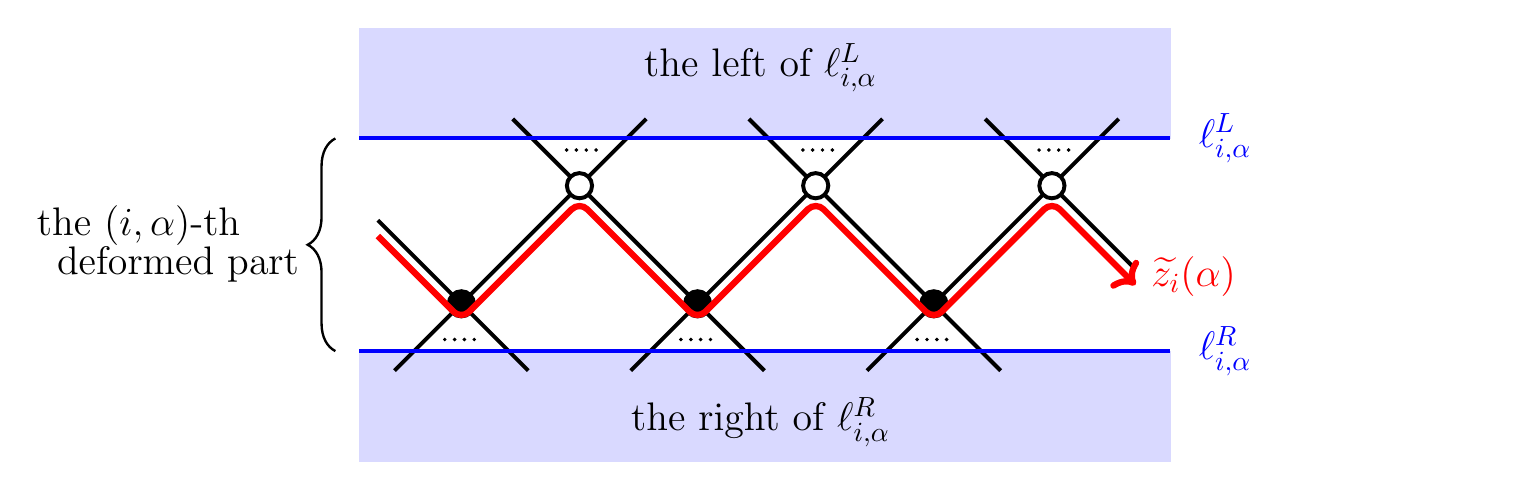
\begin{tikzpicture}[sarrow/.style={black, -latex, very thick},tarrow/.style={black, latex-, very thick}]
\newcommand{\edgewidth}{0.05cm} %line_width_of _edges
\newcommand{\nodewidth}{0.05cm} %line_width_around_nodes
\newcommand{\noderad}{0.16} %radius_of_node

%coordinate setting
\coordinate (B1) at (0,0); \coordinate (B2) at (3,0); \coordinate (B3) at (6,0);
\coordinate (W1) at (1.5,1.5); \coordinate (W2) at (4.5,1.5); \coordinate (W3) at (7.5,1.5);

\path (B1) ++(135:1.5cm) coordinate (B1w); \path (B1) ++(225:1.2cm) coordinate (B1s); \path (B1) ++(315:1.2cm) coordinate (B1e);
\path (W1) ++(45:1.2cm) coordinate (W1w); \path (W1) ++(135:1.2cm) coordinate (W1s);
\path (B2) ++(225:1.2cm) coordinate (B2s); \path (B2) ++(315:1.2cm) coordinate (B2e);
\path (W2) ++(45:1.2cm) coordinate (W2w); \path (W2) ++(135:1.2cm) coordinate (W2s);
\path (B3) ++(225:1.2cm) coordinate (B3s); \path (B3) ++(315:1.2cm) coordinate (B3e);
\path (W3) ++(315:1.5cm) coordinate (W3n);
\path (W3) ++(45:1.2cm) coordinate (W3w); \path (W3) ++(135:1.2cm) coordinate (W3s);

\path (B1) ++(245:0.5cm) coordinate (B1ss); \path (B1) ++(295:0.5cm) coordinate (B1ee);
\path (W1) ++(65:0.5cm) coordinate (W1ww); \path (W1) ++(115:0.5cm) coordinate (W1ss);
\path (B2) ++(245:0.5cm) coordinate (B2ss); \path (B2) ++(295:0.5cm) coordinate (B2ee);
\path (W2) ++(65:0.5cm) coordinate (W2ww); \path (W2) ++(115:0.5cm) coordinate (W2ss);
\path (B3) ++(245:0.5cm) coordinate (B3ss); \path (B3) ++(295:0.5cm) coordinate (B3ee);
\path (W3) ++(65:0.5cm) coordinate (W3ww); \path (W3) ++(115:0.5cm) coordinate (W3ss);

%irrelevant part
\filldraw[blue!15, fill=blue!15] (-1.3,2.1)--(9,2.1)--(9,3.5)--(-1.3,3.5);
\filldraw[blue!15, fill=blue!15] (-1.3,-0.6)--(9,-0.6)--(9,-2)--(-1.3,-2);
%edge
\draw [line width=\edgewidth] (B1w)--(B1)--(W1)--(B2)--(W2)--(B3)--(W3)--(W3n);
\draw [line width=\edgewidth] (B1s)--(B1)--(B1e); \draw[line width=\edgewidth] (B2s)--(B2)--(B2e); \draw [line width=\edgewidth] (B3s)--(B3)--(B3e);
\draw [line width=\edgewidth] (W1w)--(W1)--(W1s); \draw[line width=\edgewidth] (W2w)--(W2)--(W2s); \draw [line width=\edgewidth] (W3w)--(W3)--(W3s);

\draw [line width=\edgewidth,line cap=round, dash pattern=on 0pt off 2.5\pgflinewidth] (B1ss)--(B1ee);
\draw [line width=\edgewidth,line cap=round, dash pattern=on 0pt off 2.5\pgflinewidth] (W1ww)--(W1ss);
\draw [line width=\edgewidth,line cap=round, dash pattern=on 0pt off 2.5\pgflinewidth] (B2ss)--(B2ee);
\draw [line width=\edgewidth,line cap=round, dash pattern=on 0pt off 2.5\pgflinewidth] (W2ww)--(W2ss);
\draw [line width=\edgewidth,line cap=round, dash pattern=on 0pt off 2.5\pgflinewidth] (B3ss)--(B3ee);
\draw [line width=\edgewidth,line cap=round, dash pattern=on 0pt off 2.5\pgflinewidth] (W3ww)--(W3ss);
%blacknode
\draw [line width=\nodewidth, fill=black] (B1) circle [radius=\noderad] ;
\draw [line width=\nodewidth, fill=black] (B2) circle [radius=\noderad] ;
\draw [line width=\nodewidth, fill=black] (B3) circle [radius=\noderad] ;
%whitenode
\draw [line width=\nodewidth, fill=white] (W1) circle [radius=\noderad] ;
\draw [line width=\nodewidth, fill=white] (W2) circle [radius=\noderad] ;
\draw [line width=\nodewidth, fill=white] (W3) circle [radius=\noderad] ;
%zigzag
\path (B1w) ++(-90:0.2cm) coordinate (B1w+);
\path (B1) ++(-90:0.2cm) coordinate (B1+); \path (W1) ++(-90:0.2cm) coordinate (W1+);
\path (B2) ++(-90:0.2cm) coordinate (B2+); \path (W2) ++(-90:0.2cm) coordinate (W2+);
\path (B3) ++(-90:0.2cm) coordinate (B3+); \path (W3) ++(-90:0.2cm) coordinate (W3+);
\path (W3n) ++(-90:0.2cm) coordinate (W3n+);
\draw [->, rounded corners, line width=0.08cm, red] (B1w+)--(B1+)--(W1+)--(B2+)--(W2+)--(B3+)--(W3+)--(W3n+) ;
%line
\draw[line width=0.05cm, blue] (-1.3,2.1)--(9,2.1); \draw[line width=0.05cm, blue] (-1.3,-0.6)--(9,-0.6);
%node
\node[red] at (9.3,0.35) {\Large$\widetilde{z_i}(\alpha)$} ;
\node[blue] at (9.7,2.1) {\Large $\ell_{i,\alpha}^L$} ; \node[blue] at (9.7,-0.6) {\Large $\ell_{i,\alpha}^R$} ;

\node at (3.8,3) {\Large the left of $\ell_{i,\alpha}^L$} ; \node at (3.8,-1.5) {\Large the right of $\ell_{i,\alpha}^R$} ;
\draw [line width=0.03cm, decorate, decoration={brace, mirror, amplitude=10pt}](-1.6,2.1) -- (-1.6,-0.6) node[black,midway,xshift=-2.5cm,yshift=0.25cm] {\Large the $(i,\alpha)$-th} node[black,midway,xshift=-2cm,yshift=-0.25cm] {\Large deformed part};
%modify the space
\node at (13,0) {};
\end{tikzpicture}
} }
\caption{}\label{def_leftright}
\end{figure}

Also, we call the region obtained as the intersection of the right of $\ell_{i-1,\alpha}^R$ and the left of $\ell_{i,\alpha}^L$ the \emph{$(i,\alpha)$-th irrelevant part}.
Here, we say that the intersection of the right of $\ell_{r,\alpha}^R$ and the left of $\ell_{1,\alpha+1}^L$ is the \emph{$(1,\alpha+1)$-th irrelevant part}.
We remark that sometimes there are no nodes in an irrelevant part. We sometimes omit $\alpha\in\ZZ$ from the notation unless it causes confusion.
We also use these terminologies for~$\Gamma$.
That is, a part of~$\Gamma$ obtained by projecting a deformed (resp.\ irrelevant) part of $\widetilde{\Gamma}$ onto $\Gamma$ is said to be a \emph{deformed} (resp.\ \emph{irrelevant}) \emph{part} of~$\Gamma$.

\begin{figure}[h!]\centering
{\scalebox{0.6}{
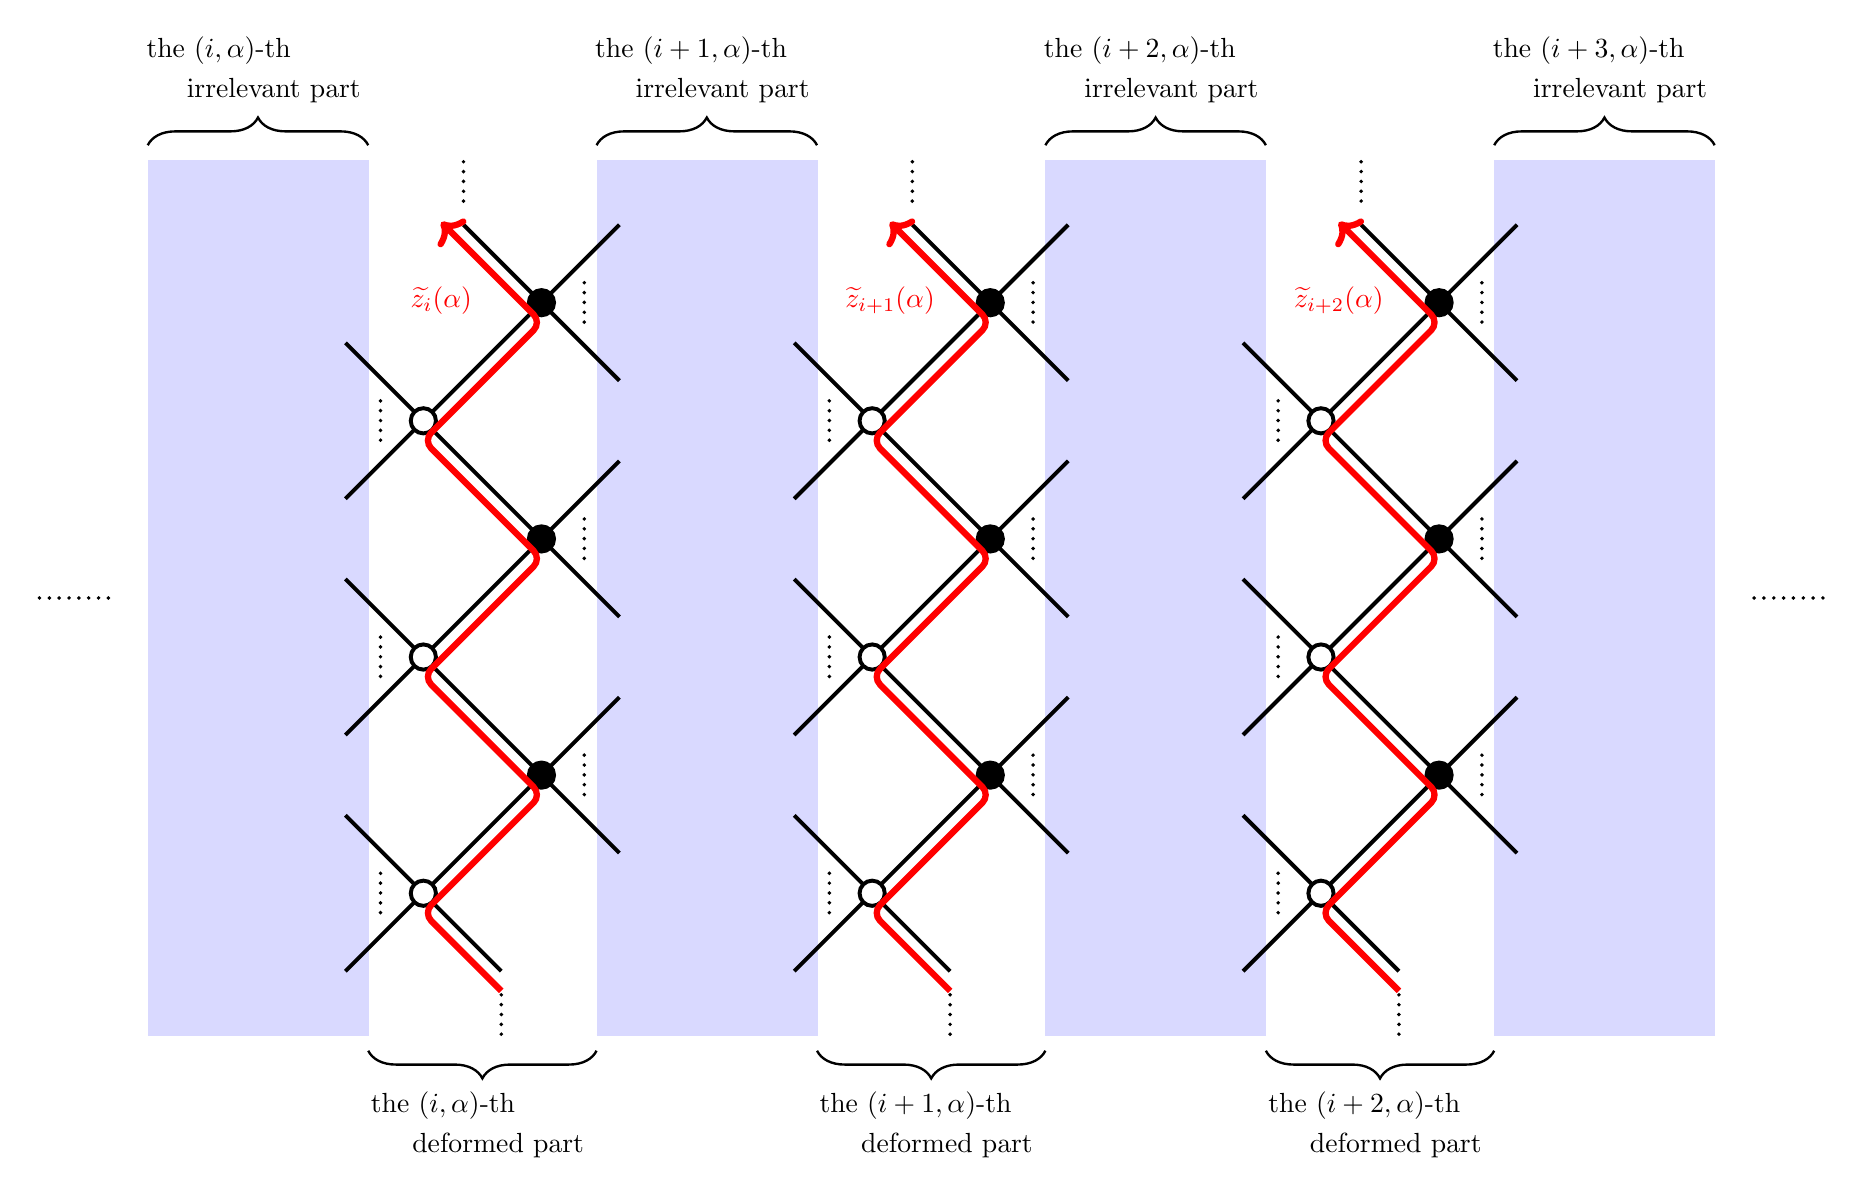
\begin{tikzpicture}
\newcommand{\edgewidth}{0.05cm} %line_width_of _edges
\newcommand{\nodewidth}{0.05cm} %line_width_around_nodes
\newcommand{\noderad}{0.16} %radius_of_node

%deform and irrelevant part I
\filldraw[blue!15, fill=blue!15] (-3.5,-1.8)--(-0.7,-1.8)--(-0.7,9.3)--(-3.5,9.3);
\draw [line width=0.03cm, decorate, decoration={brace, amplitude=10pt}](-3.5,9.5)--(-0.7,9.5) node[black,midway,xshift=-0.5cm,yshift=1.2cm] {the $(i,\alpha)$-th} node[black,midway,xshift=0.2cm,yshift=0.7cm] {irrelevant part};

\draw [line width=0.03cm, decorate, decoration={brace, mirror, amplitude=10pt}](-0.7,-2)--(2.2,-2) node[black,midway,xshift=-0.5cm,yshift=-0.7cm] {the $(i,\alpha)$-th} node[black,midway,xshift=0.2cm,yshift=-1.2cm] {deformed part};

%deform and irrelevant part II
\filldraw[blue!15, fill=blue!15] (2.2,-1.8)--(5,-1.8)--(5,9.3)--(2.2,9.3);
\draw [line width=0.03cm, decorate, decoration={brace, amplitude=10pt}](2.2,9.5)--(5,9.5) node[black,midway,xshift=-0.2cm,yshift=1.2cm] {the $(i+1,\alpha)$-th} node[black,midway,xshift=0.2cm,yshift=0.7cm] {irrelevant part};

\draw [line width=0.03cm, decorate, decoration={brace, mirror, amplitude=10pt}](5,-2)--(7.9,-2) node[black,midway,xshift=-0.2cm,yshift=-0.7cm] {the $(i+1,\alpha)$-th} node[black,midway,xshift=0.2cm,yshift=-1.2cm] {deformed part};

%deform and irrelevant part III
\filldraw[blue!15, fill=blue!15] (7.9,-1.8)--(10.7,-1.8)--(10.7,9.3)--(7.9,9.3);
\draw [line width=0.03cm, decorate, decoration={brace, amplitude=10pt}](7.9,9.5)--(10.7,9.5) node[black,midway,xshift=-0.2cm,yshift=1.2cm] {the $(i+2,\alpha)$-th} node[black,midway,xshift=0.2cm,yshift=0.7cm] {irrelevant part};

\draw [line width=0.03cm, decorate, decoration={brace, mirror, amplitude=10pt}](10.7,-2)--(13.6,-2) node[black,midway,xshift=-0.2cm,yshift=-0.7cm] {the $(i+2,\alpha)$-th} node[black,midway,xshift=0.2cm,yshift=-1.2cm] {deformed part};

%deform and irrelevant part IV
\filldraw[blue!15, fill=blue!15] (13.6,-1.8)--(16.4,-1.8)--(16.4,9.3)--(13.6,9.3);
\draw [line width=0.03cm, decorate, decoration={brace, amplitude=10pt}](13.6,9.5)--(16.4,9.5) node[black,midway,xshift=-0.2cm,yshift=1.2cm] {the $(i+3,\alpha)$-th} node[black,midway,xshift=0.2cm,yshift=0.7cm] {irrelevant part};

\draw [line width=\edgewidth,line cap=round, dash pattern=on 0pt off 2.5\pgflinewidth] (-4,3.75)--(-5,3.75);
\draw [line width=\edgewidth,line cap=round, dash pattern=on 0pt off 2.5\pgflinewidth] (16.9,3.75)--(17.9,3.75);

%deformed part I
%coordinate setting
\coordinate (W1) at (0,0); \coordinate (W2) at (0,3); \coordinate (W3) at (0,6);
\coordinate (B1) at (1.5,1.5); \coordinate (B2) at (1.5,4.5); \coordinate (B3) at (1.5,7.5);

\path (W1) ++(135:1.4cm) coordinate (W1w); \path (W1) ++(225:1.4cm) coordinate (W1s); \path (W1) ++(315:1.4cm) coordinate (W1e);
\path (B1) ++(45:1.4cm) coordinate (B1e); \path (B1) ++(315:1.4cm) coordinate (B1s);
\path (W2) ++(135:1.4cm) coordinate (W2w); \path (W2) ++(225:1.4cm) coordinate (W2s);
\path (B2) ++(45:1.4cm) coordinate (B2e); \path (B2) ++(315:1.4cm) coordinate (B2s);
\path (W3) ++(135:1.4cm) coordinate (W3w); \path (W3) ++(225:1.4cm) coordinate (W3s);
\path (B3) ++(45:1.4cm) coordinate (B3e); \path (B3) ++(315:1.4cm) coordinate (B3s); \path (B3) ++(135:1.4cm) coordinate (B3n);

\path (W1) ++(155:0.6cm) coordinate (W1+); \path (W1) ++(205:0.6cm) coordinate (W1-);
\path (W2) ++(155:0.6cm) coordinate (W2+); \path (W2) ++(205:0.6cm) coordinate (W2-);
\path (W3) ++(155:0.6cm) coordinate (W3+); \path (W3) ++(205:0.6cm) coordinate (W3-);
\path (B1) ++(25:0.6cm) coordinate (B1+); \path (B1) ++(335:0.6cm) coordinate (B1-);
\path (B2) ++(25:0.6cm) coordinate (B2+); \path (B2) ++(335:0.6cm) coordinate (B2-);
\path (B3) ++(25:0.6cm) coordinate (B3+); \path (B3) ++(335:0.6cm) coordinate (B3-);
%edge
\draw [line width=\edgewidth] (W1)--(B1)--(W2)--(B2)--(W3)--(B3) ;

\draw [line width=\edgewidth] (W1)--(W1w); \draw [line width=\edgewidth] (W1)--(W1s); \draw [line width=\edgewidth] (W1)--(W1e);
\draw [line width=\edgewidth] (B1)--(B1e); \draw [line width=\edgewidth] (B1)--(B1s);
\draw [line width=\edgewidth] (W2)--(W2w); \draw [line width=\edgewidth] (W2)--(W2s);
\draw [line width=\edgewidth] (B2)--(B2e); \draw [line width=\edgewidth] (B2)--(B2s);
\draw [line width=\edgewidth] (W3)--(W3w); \draw [line width=\edgewidth] (W3)--(W3s);
\draw [line width=\edgewidth] (B3)--(B3e); \draw [line width=\edgewidth] (B3)--(B3s); \draw [line width=\edgewidth] (B3)--(B3n);

\draw [line width=\edgewidth,line cap=round, dash pattern=on 0pt off 2.5\pgflinewidth] (W1+)--(W1-);
\draw [line width=\edgewidth,line cap=round, dash pattern=on 0pt off 2.5\pgflinewidth] (W2+)--(W2-);
\draw [line width=\edgewidth,line cap=round, dash pattern=on 0pt off 2.5\pgflinewidth] (W3+)--(W3-);
\draw [line width=\edgewidth,line cap=round, dash pattern=on 0pt off 2.5\pgflinewidth] (B1+)--(B1-);
\draw [line width=\edgewidth,line cap=round, dash pattern=on 0pt off 2.5\pgflinewidth] (B2+)--(B2-);
\draw [line width=\edgewidth,line cap=round, dash pattern=on 0pt off 2.5\pgflinewidth] (B3+)--(B3-);

\path (W1e) ++(-90:0.3cm) coordinate (W1e_dot); \path (W1e) ++(-90:0.9cm) coordinate (W1e_ddot);
\draw [line width=\edgewidth,line cap=round, dash pattern=on 0pt off 2.5\pgflinewidth] (W1e_dot)--(W1e_ddot);
\path (B3n) ++(90:0.3cm) coordinate (B3n_dot); \path (B3n) ++(90:0.9cm) coordinate (B3n_ddot);
\draw [line width=\edgewidth,line cap=round, dash pattern=on 0pt off 2.5\pgflinewidth] (B3n_dot)--(B3n_ddot);

%blacknode
\draw [line width=\nodewidth, fill=black] (B1) circle [radius=\noderad] ;
\draw [line width=\nodewidth, fill=black] (B2) circle [radius=\noderad] ;
\draw [line width=\nodewidth, fill=black] (B3) circle [radius=\noderad] ;
%whitenode
\draw [line width=\nodewidth, fill=white] (W1) circle [radius=\noderad] ;
\draw [line width=\nodewidth, fill=white] (W2) circle [radius=\noderad] ;
\draw [line width=\nodewidth, fill=white] (W3) circle [radius=\noderad] ;
%zigzag
\path (W1e) ++(-90:0.25cm) coordinate (W1ez);
\path (B1) ++(-90:0.25cm) coordinate (B1z); \path (W1) ++(-90:0.25cm) coordinate (W1z);
\path (B2) ++(-90:0.25cm) coordinate (B2z); \path (W2) ++(-90:0.25cm) coordinate (W2z);
\path (B3) ++(-90:0.25cm) coordinate (B3z); \path (W3) ++(-90:0.25cm) coordinate (W3z);
\path (B3) ++(135:1.8cm) coordinate (B3nn); \path (B3nn) ++(-90:0.25cm) coordinate (B3nz);
\draw [->, rounded corners, line width=0.08cm, red] (W1ez)--(W1z)--(B1z)--(W2z)--(B2z)--(W3z)--(B3z)--(B3nz) ;
%node
\path (B3nz) ++(-90:1cm) coordinate (zi);\node[red] at (zi) {$\widetilde{z_i}(\alpha)$} ;

%deformed part II
%coordinate setting
\coordinate (W1) at (5.7,0); \coordinate (W2) at (5.7,3); \coordinate (W3) at (5.7,6);
\coordinate (B1) at (7.2,1.5); \coordinate (B2) at (7.2,4.5); \coordinate (B3) at (7.2,7.5);

\path (W1) ++(135:1.4cm) coordinate (W1w); \path (W1) ++(225:1.4cm) coordinate (W1s); \path (W1) ++(315:1.4cm) coordinate (W1e);
\path (B1) ++(45:1.4cm) coordinate (B1e); \path (B1) ++(315:1.4cm) coordinate (B1s);
\path (W2) ++(135:1.4cm) coordinate (W2w); \path (W2) ++(225:1.4cm) coordinate (W2s);
\path (B2) ++(45:1.4cm) coordinate (B2e); \path (B2) ++(315:1.4cm) coordinate (B2s);
\path (W3) ++(135:1.4cm) coordinate (W3w); \path (W3) ++(225:1.4cm) coordinate (W3s);
\path (B3) ++(45:1.4cm) coordinate (B3e); \path (B3) ++(315:1.4cm) coordinate (B3s); \path (B3) ++(135:1.4cm) coordinate (B3n);

\path (W1) ++(155:0.6cm) coordinate (W1+); \path (W1) ++(205:0.6cm) coordinate (W1-);
\path (W2) ++(155:0.6cm) coordinate (W2+); \path (W2) ++(205:0.6cm) coordinate (W2-);
\path (W3) ++(155:0.6cm) coordinate (W3+); \path (W3) ++(205:0.6cm) coordinate (W3-);
\path (B1) ++(25:0.6cm) coordinate (B1+); \path (B1) ++(335:0.6cm) coordinate (B1-);
\path (B2) ++(25:0.6cm) coordinate (B2+); \path (B2) ++(335:0.6cm) coordinate (B2-);
\path (B3) ++(25:0.6cm) coordinate (B3+); \path (B3) ++(335:0.6cm) coordinate (B3-);
%edge
\draw [line width=\edgewidth] (W1)--(B1)--(W2)--(B2)--(W3)--(B3) ;

\draw [line width=\edgewidth] (W1)--(W1w); \draw [line width=\edgewidth] (W1)--(W1s); \draw [line width=\edgewidth] (W1)--(W1e);
\draw [line width=\edgewidth] (B1)--(B1e); \draw [line width=\edgewidth] (B1)--(B1s);
\draw [line width=\edgewidth] (W2)--(W2w); \draw [line width=\edgewidth] (W2)--(W2s);
\draw [line width=\edgewidth] (B2)--(B2e); \draw [line width=\edgewidth] (B2)--(B2s);
\draw [line width=\edgewidth] (W3)--(W3w); \draw [line width=\edgewidth] (W3)--(W3s);
\draw [line width=\edgewidth] (B3)--(B3e); \draw [line width=\edgewidth] (B3)--(B3s); \draw [line width=\edgewidth] (B3)--(B3n);

\draw [line width=\edgewidth,line cap=round, dash pattern=on 0pt off 2.5\pgflinewidth] (W1+)--(W1-);
\draw [line width=\edgewidth,line cap=round, dash pattern=on 0pt off 2.5\pgflinewidth] (W2+)--(W2-);
\draw [line width=\edgewidth,line cap=round, dash pattern=on 0pt off 2.5\pgflinewidth] (W3+)--(W3-);
\draw [line width=\edgewidth,line cap=round, dash pattern=on 0pt off 2.5\pgflinewidth] (B1+)--(B1-);
\draw [line width=\edgewidth,line cap=round, dash pattern=on 0pt off 2.5\pgflinewidth] (B2+)--(B2-);
\draw [line width=\edgewidth,line cap=round, dash pattern=on 0pt off 2.5\pgflinewidth] (B3+)--(B3-);

\path (W1e) ++(-90:0.3cm) coordinate (W1e_dot); \path (W1e) ++(-90:0.9cm) coordinate (W1e_ddot);
\draw [line width=\edgewidth,line cap=round, dash pattern=on 0pt off 2.5\pgflinewidth] (W1e_dot)--(W1e_ddot);
\path (B3n) ++(90:0.3cm) coordinate (B3n_dot); \path (B3n) ++(90:0.9cm) coordinate (B3n_ddot);
\draw [line width=\edgewidth,line cap=round, dash pattern=on 0pt off 2.5\pgflinewidth] (B3n_dot)--(B3n_ddot);

%blacknode
\draw [line width=\nodewidth, fill=black] (B1) circle [radius=\noderad] ;
\draw [line width=\nodewidth, fill=black] (B2) circle [radius=\noderad] ;
\draw [line width=\nodewidth, fill=black] (B3) circle [radius=\noderad] ;
%whitenode
\draw [line width=\nodewidth, fill=white] (W1) circle [radius=\noderad] ;
\draw [line width=\nodewidth, fill=white] (W2) circle [radius=\noderad] ;
\draw [line width=\nodewidth, fill=white] (W3) circle [radius=\noderad] ;
%zigzag
\path (W1e) ++(-90:0.25cm) coordinate (W1ez);
\path (B1) ++(-90:0.25cm) coordinate (B1z); \path (W1) ++(-90:0.25cm) coordinate (W1z);
\path (B2) ++(-90:0.25cm) coordinate (B2z); \path (W2) ++(-90:0.25cm) coordinate (W2z);
\path (B3) ++(-90:0.25cm) coordinate (B3z); \path (W3) ++(-90:0.25cm) coordinate (W3z);
\path (B3) ++(135:1.8cm) coordinate (B3nn); \path (B3nn) ++(-90:0.25cm) coordinate (B3nz);
\draw [->, rounded corners, line width=0.08cm, red] (W1ez)--(W1z)--(B1z)--(W2z)--(B2z)--(W3z)--(B3z)--(B3nz) ;
%node
\path (B3nz) ++(-90:1cm) coordinate (zi);\node[red] at (zi) {$\widetilde{z}_{i+1}(\alpha)$} ;

%deformed part III
%coordinate setting
\coordinate (W1) at (11.4,0); \coordinate (W2) at (11.4,3); \coordinate (W3) at (11.4,6);
\coordinate (B1) at (12.9,1.5); \coordinate (B2) at (12.9,4.5); \coordinate (B3) at (12.9,7.5);

\path (W1) ++(135:1.4cm) coordinate (W1w); \path (W1) ++(225:1.4cm) coordinate (W1s); \path (W1) ++(315:1.4cm) coordinate (W1e);
\path (B1) ++(45:1.4cm) coordinate (B1e); \path (B1) ++(315:1.4cm) coordinate (B1s);
\path (W2) ++(135:1.4cm) coordinate (W2w); \path (W2) ++(225:1.4cm) coordinate (W2s);
\path (B2) ++(45:1.4cm) coordinate (B2e); \path (B2) ++(315:1.4cm) coordinate (B2s);
\path (W3) ++(135:1.4cm) coordinate (W3w); \path (W3) ++(225:1.4cm) coordinate (W3s);
\path (B3) ++(45:1.4cm) coordinate (B3e); \path (B3) ++(315:1.4cm) coordinate (B3s); \path (B3) ++(135:1.4cm) coordinate (B3n);

\path (W1) ++(155:0.6cm) coordinate (W1+); \path (W1) ++(205:0.6cm) coordinate (W1-);
\path (W2) ++(155:0.6cm) coordinate (W2+); \path (W2) ++(205:0.6cm) coordinate (W2-);
\path (W3) ++(155:0.6cm) coordinate (W3+); \path (W3) ++(205:0.6cm) coordinate (W3-);
\path (B1) ++(25:0.6cm) coordinate (B1+); \path (B1) ++(335:0.6cm) coordinate (B1-);
\path (B2) ++(25:0.6cm) coordinate (B2+); \path (B2) ++(335:0.6cm) coordinate (B2-);
\path (B3) ++(25:0.6cm) coordinate (B3+); \path (B3) ++(335:0.6cm) coordinate (B3-);
%edge
\draw [line width=\edgewidth] (W1)--(B1)--(W2)--(B2)--(W3)--(B3) ;

\draw [line width=\edgewidth] (W1)--(W1w); \draw [line width=\edgewidth] (W1)--(W1s); \draw [line width=\edgewidth] (W1)--(W1e);
\draw [line width=\edgewidth] (B1)--(B1e); \draw [line width=\edgewidth] (B1)--(B1s);
\draw [line width=\edgewidth] (W2)--(W2w); \draw [line width=\edgewidth] (W2)--(W2s);
\draw [line width=\edgewidth] (B2)--(B2e); \draw [line width=\edgewidth] (B2)--(B2s);
\draw [line width=\edgewidth] (W3)--(W3w); \draw [line width=\edgewidth] (W3)--(W3s);
\draw [line width=\edgewidth] (B3)--(B3e); \draw [line width=\edgewidth] (B3)--(B3s); \draw [line width=\edgewidth] (B3)--(B3n);

\draw [line width=\edgewidth,line cap=round, dash pattern=on 0pt off 2.5\pgflinewidth] (W1+)--(W1-);
\draw [line width=\edgewidth,line cap=round, dash pattern=on 0pt off 2.5\pgflinewidth] (W2+)--(W2-);
\draw [line width=\edgewidth,line cap=round, dash pattern=on 0pt off 2.5\pgflinewidth] (W3+)--(W3-);
\draw [line width=\edgewidth,line cap=round, dash pattern=on 0pt off 2.5\pgflinewidth] (B1+)--(B1-);
\draw [line width=\edgewidth,line cap=round, dash pattern=on 0pt off 2.5\pgflinewidth] (B2+)--(B2-);
\draw [line width=\edgewidth,line cap=round, dash pattern=on 0pt off 2.5\pgflinewidth] (B3+)--(B3-);

\path (W1e) ++(-90:0.3cm) coordinate (W1e_dot); \path (W1e) ++(-90:0.9cm) coordinate (W1e_ddot);
\draw [line width=\edgewidth,line cap=round, dash pattern=on 0pt off 2.5\pgflinewidth] (W1e_dot)--(W1e_ddot);
\path (B3n) ++(90:0.3cm) coordinate (B3n_dot); \path (B3n) ++(90:0.9cm) coordinate (B3n_ddot);
\draw [line width=\edgewidth,line cap=round, dash pattern=on 0pt off 2.5\pgflinewidth] (B3n_dot)--(B3n_ddot);

%blacknode
\draw [line width=\nodewidth, fill=black] (B1) circle [radius=\noderad] ;
\draw [line width=\nodewidth, fill=black] (B2) circle [radius=\noderad] ;
\draw [line width=\nodewidth, fill=black] (B3) circle [radius=\noderad] ;
%whitenode
\draw [line width=\nodewidth, fill=white] (W1) circle [radius=\noderad] ;
\draw [line width=\nodewidth, fill=white] (W2) circle [radius=\noderad] ;
\draw [line width=\nodewidth, fill=white] (W3) circle [radius=\noderad] ;
%zigzag
\path (W1e) ++(-90:0.25cm) coordinate (W1ez);
\path (B1) ++(-90:0.25cm) coordinate (B1z); \path (W1) ++(-90:0.25cm) coordinate (W1z);
\path (B2) ++(-90:0.25cm) coordinate (B2z); \path (W2) ++(-90:0.25cm) coordinate (W2z);
\path (B3) ++(-90:0.25cm) coordinate (B3z); \path (W3) ++(-90:0.25cm) coordinate (W3z);
\path (B3) ++(135:1.8cm) coordinate (B3nn); \path (B3nn) ++(-90:0.25cm) coordinate (B3nz);
\draw [->, rounded corners, line width=0.08cm, red] (W1ez)--(W1z)--(B1z)--(W2z)--(B2z)--(W3z)--(B3z)--(B3nz) ;
%node
\path (B3nz) ++(-90:1cm) coordinate (zi); \node[red] at (zi) {$\widetilde{z}_{i+2}(\alpha)$} ;
\end{tikzpicture}
} }
\caption{}
\label{fig_deformed_irrelevant}
\end{figure}

By the condition of Definition~\ref{def_properly}(3), $z_1,\dots,z_r$ do not have a common node, and therefore the irrelevant parts do not overlap each other.
Since the operations (zig-1)--(zig-4) (or (zag-1)--(zag-4)) are local operations on each deformed part, any irrelevant part will be unchanged even if we apply these operations.
Thus, we continue to use these terminologies ``deformed parts’’ and ``irrelevant parts’’.
We then consider a zigzag path $w$ satisfying the following properties:
\begin{itemize}\itemsep=0pt
\item[(a)] If $[z_i]$ and $[w]$ are linearly independent, then by Lemma~\ref{slope_linearly_independent}, $\widetilde{w}$ intersects with $\widetilde{z_i}(\alpha)$ precisely once, and so does any $\widetilde{z_i}(\alpha)$ with $i=1,\dots,r$ and $\alpha\in\ZZ$.
In particular, all intersections are zigs of $w$ or zags of $w$ by Lemma~\ref{intersect_zigorzag2}.
If $\widetilde{w}$ intersects with $\widetilde{z_i}(\alpha)$ at a zig (resp.\ zag) of $\widetilde{z_i}(\alpha)$, then we easily see that $\widetilde{w}$ crosses the $(i,\alpha)$-th deformed part in the direction from the $(i,\alpha)$-th (resp.~$(i+1,\alpha)$-th) irrelevant part to the $(i+1,\alpha)$-th (resp.~$(i,\alpha)$-th) irrelevant part.

\item[(b)] If $[z_i]$ and $[w]$ are linearly dependent, then by Lemma~\ref{slope_linearly_independent}, $\widetilde{w}$ and $\widetilde{z_i}(\alpha)$ do not intersect for any $i=1,\dots,r$ and $\alpha\in\ZZ$.
This is equivalent to the condition that $\widetilde{w}$ is contained in some irrelevant part.
In this case, $w$ is unchanged even if we apply the extended deformations because (zig-1)--(zig-4) (or (zag-1)--(zag-4)) are operations on the deformed parts, and~(zig-5) (or~(zag-5)) does not affect $w$ by Lemma~\ref{bypass_removable} below.
\end{itemize}
\end{observation}

In the remainder of this subsection, we discuss the behavior of zigzag paths after applying the operations (zig-1)--(zig-4).
(We can apply the same arguments for the case of (zag-1)--(zag-4).)

\begin{observation}\label{obs_deformed_part2}
We consider a zigzag path $y_k$ on a consistent dimer model $\Gamma$ intersecting with $z_i$ at a zig of $z_i$.
Let $\widetilde{z}_i$ and $\widetilde{y}_k$ be zigzag paths on $\widetilde{\Gamma}$ projecting onto $z_i$ and $y_k$, respectively.
By Observation~\ref{obs_deformed_part}(a), $\widetilde{y}_k$ crosses the $i$-th deformed part in the direction from the $i$-th irrelevant part to the $(i+1)$-th irrelevant part, and $\widetilde{y}_k$ intersects with $\widetilde{z_i}$ precisely once.
We suppose that the zig $\widetilde{z_i}[2m-1]$ of $\widetilde{z_i}$ is such an intersection.
In this case, $\widetilde{z_i}[2m-1]$ is also a zag of $\widetilde{y}_k$; thus we may write it as~$\widetilde{y_k}[2m]$.

Now, we apply the operations (zig-1)--(zig-3) to~$\Gamma$, and we denote the resulting dimer model by~$\Gamma^\prime$ and its universal cover by~$\widetilde{\Gamma}^\prime$.
Then, some new nodes are inserted in $\widetilde{z_i}[2m-1]=\widetilde{y_k}[2m]$, and zigzag paths $\widetilde{z}_{i,1},\dots,\widetilde{z}_{i,p_i}$ on $\widetilde{\Gamma}^\prime$, which project onto zigzag paths $z_{i,1},\dots,z_{i,p_i}$ on~$\Gamma^\prime$, respectively, appear in the $i$-th deformed part.

\begin{figure}[h!]\centering
\begin{tikzpicture}
\node at (-0.5,0)
{\scalebox{0.7}{
\begin{tikzpicture}
\newcommand{\edgewidth}{0.05cm} %line_width_of _edges
\newcommand{\nodewidth}{0.05cm} %line_width_around_nodes
\newcommand{\noderad}{0.16} %radius_of_node

%coordinate setting
\coordinate (W1) at (0,0); \coordinate (B1) at (2.5,0);
\path (W1) ++(135:1.5cm) coordinate (W1a); \path (W1) ++(150:1.5cm) coordinate (W1a-); \path (W1) ++(225:1.5cm) coordinate (W1b);
\path (B1) ++(45:1.5cm) coordinate (B1a); \path (B1) ++(330:1.5cm) coordinate (B1a-); \path (B1) ++(315:1.5cm) coordinate (B1b);

%edge
\draw [line width=\edgewidth] (W1)--(B1);
\draw [line width=\edgewidth] (W1)--(W1a); \draw [line width=\edgewidth] (W1)--(W1a-); \draw [line width=\edgewidth] (W1)--(W1b);
\draw [line width=\edgewidth] (B1)--(B1a); \draw [line width=\edgewidth] (B1)--(B1a-); \draw [line width=\edgewidth] (B1)--(B1b);
\draw [line width=\edgewidth,line cap=round, dash pattern=on 0pt off 2.5\pgflinewidth] (-1,0.25)--(-1,-0.45);
\draw [line width=\edgewidth,line cap=round, dash pattern=on 0pt off 2.5\pgflinewidth] (3.5,0.45)--(3.5,-0.25);

%node
\draw [line width=\nodewidth, fill=white] (W1) circle [radius=\noderad] ;
\draw [line width=\nodewidth, fill=black] (B1) circle [radius=\noderad] ;

%zigzag
\path (W1) ++(270:0.3cm) coordinate (W1-); \path (W1) ++(90:0.3cm) coordinate (W1+);
\path (B1) ++(270:0.3cm) coordinate (B1-); \path (B1) ++(90:0.3cm) coordinate (B1+);
\path (W1-) ++(225:1.7cm) coordinate (W1--); \path (W1+) ++(135:1.7cm) coordinate (W1++);
\path (B1-) ++(315:1.7cm) coordinate (B1--); \path (B1+) ++(45:1.7cm) coordinate (B1++);

\draw [->, rounded corners, line width=0.08cm, red] (B1--)--(B1-)--(W1+)--(W1++) ;
\draw [->, rounded corners, line width=0.08cm, blue] (W1--)--(W1-)--(B1+)--(B1++) ;

%node
\node[blue] at (3,1.3) {\Large$\widetilde{y}_k$};
\node[red] at (-0.5,1.3) {\Large$\widetilde{z}_i$};
\end{tikzpicture}
} };

\draw [->,line width=0.035cm] (2.2,0)--(4.8,0);
%\node at (3.5,0.5) {$\nu_\bfp^\zig$};
\node at (3.5,0.35) {\small(zig-1)--(zig-3)};

\node at (8.5,0)
{\scalebox{0.7}{
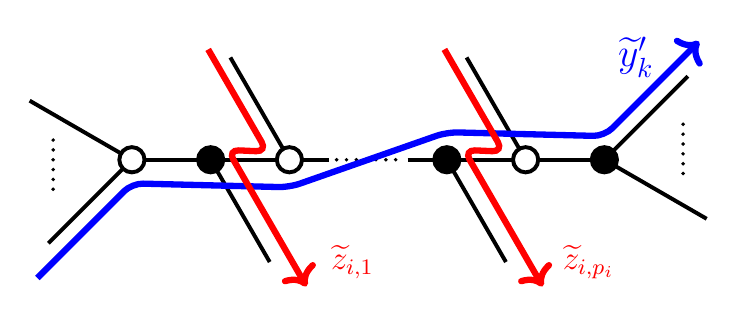
\begin{tikzpicture}
\newcommand{\edgewidth}{0.05cm} %line_width_of _edges
\newcommand{\nodewidth}{0.05cm} %line_width_around_nodes
\newcommand{\noderad}{0.16} %radius_of_node

%coordinate setting
\coordinate (W1) at (0,0); \coordinate (B1) at (6,0);
\path (W1) ++(135:1.5cm) coordinate (W1a); \path (W1) ++(150:1.5cm) coordinate (W1a-); \path (W1) ++(225:1.5cm) coordinate (W1b);
\path (B1) ++(45:1.5cm) coordinate (B1a); \path (B1) ++(330:1.5cm) coordinate (B1a-); \path (B1) ++(315:1.5cm) coordinate (B1b);

\coordinate (W2) at (2,0); \coordinate (W3) at (5,0);
\coordinate (B2) at (1,0); \coordinate (B3) at (4,0);

\path (W2) ++(120:1.5cm) coordinate (W2+); \path (W3) ++(120:1.5cm) coordinate (W3+);
\path (B2) ++(300:1.5cm) coordinate (B2+); \path (B3) ++(300:1.5cm) coordinate (B3+);

%edge
\draw [line width=\edgewidth] (W1)--(2.5,0); \draw [line width=\edgewidth] (3.5,0)--(B1);
\draw [line width=\edgewidth,line cap=round, dash pattern=on 0pt off 2.5\pgflinewidth] (2.6,0)--(3.4,0);
\draw [line width=\edgewidth] (W1)--(W1a-); \draw [line width=\edgewidth] (W1)--(W1b);
\draw [line width=\edgewidth] (B1)--(B1a); \draw [line width=\edgewidth] (B1)--(B1a-);
\draw [line width=\edgewidth,line cap=round, dash pattern=on 0pt off 2.5\pgflinewidth] (-1,0.25)--(-1,-0.45);
\draw [line width=\edgewidth,line cap=round, dash pattern=on 0pt off 2.5\pgflinewidth] (7,0.45)--(7,-0.25);

\draw [line width=\edgewidth] (B2)--(B2+); \draw [line width=\edgewidth] (B3)--(B3+);
\draw [line width=\edgewidth] (W2)--(W2+); \draw [line width=\edgewidth] (W3)--(W3+);

%node
\draw [line width=\nodewidth, fill=white] (W1) circle [radius=\noderad] ;
\draw [line width=\nodewidth, fill=black] (B1) circle [radius=\noderad] ;

\draw [line width=\nodewidth, fill=white] (W2) circle [radius=\noderad] ; \draw [line width=\nodewidth, fill=white] (W3) circle [radius=\noderad] ;
\draw [line width=\nodewidth, fill=black] (B2) circle [radius=\noderad] ; \draw [line width=\nodewidth, fill=black] (B3) circle [radius=\noderad] ;

%zigzag
\path (W1) ++(270:0.3cm) coordinate (W1-); \path (W1) ++(90:0.3cm) coordinate (W1+);
\path (B1) ++(270:0.3cm) coordinate (B1-); \path (B1) ++(90:0.3cm) coordinate (B1+);
\path (W1-) ++(225:1.7cm) coordinate (W1--); \path (W1+) ++(135:1.7cm) coordinate (W1++);
\path (B1-) ++(315:1.7cm) coordinate (B1--); \path (B1+) ++(45:1.7cm) coordinate (B1++);
\draw [->, rounded corners, line width=0.08cm, blue] (W1--)--(W1-)--(2,-0.35)--(4,0.35)--(B1+)--(B1++) ;

\path (B2) ++(30:0.25cm) coordinate (B2z); \path (W2) ++(160:0.3cm) coordinate (W2z);
\path (B2z) ++(300:2cm) coordinate (B2zz); \path (W2z) ++(120:1.5cm) coordinate (W2zz);
\draw [<-, rounded corners, line width=0.08cm, red] (B2zz)--(B2z)--(W2z)--(W2zz);

\path (B3) ++(30:0.25cm) coordinate (B3z); \path (W3) ++(160:0.3cm) coordinate (W3z);
\path (B3z) ++(300:2cm) coordinate (B3zz); \path (W3z) ++(120:1.5cm) coordinate (W3zz);
\draw [<-, rounded corners, line width=0.08cm, red] (B3zz)--(B3z)--(W3z)--(W3zz);
%node
\node[blue] at (6.4,1.3) {\Large$\widetilde{y}^\prime_k$};
\node[red] at (2.8,-1.3) {\large$\widetilde{z}_{i,1}$}; \node[red] at (5.8,-1.3) {\large$\widetilde{z}_{i,p_i}$};
\end{tikzpicture}
} };
\end{tikzpicture}
\caption{}\label{fig_observation_zigzag1}
\end{figure}
We consider the zigzag path $\widetilde{y}^\prime_k$ on $\widetilde{\Gamma}^\prime$ passing through $\widetilde{y_k}[2m-1]$ as a zig.
That is, $\widetilde{y}^\prime_k$ starts from $\widetilde{y_k}[2m-1]$, crosses through zigzag paths $\widetilde{z}_{i,1},\dots,\widetilde{z}_{i,p_i}$ in the $i$-th deformed part, and arrives at $\widetilde{y_k}[2m+1]$ (see the right of Figure~\ref{fig_observation_zigzag1}).
In particular, it crosses the $i$-th deformed part in the direction from the $i$-th irrelevant part to the $(i+1)$-th irrelevant part.
Although $\widetilde{y}^\prime_k$ looks different from $\widetilde{y}_k$ in the deformed parts, it connects the zigs $\widetilde{y_k}[2m-1]$ and $\widetilde{y_k}[2m+1]$ of $\widetilde{y}_k$ in the $i$-th deformed part for all $i$, and thus $\widetilde{y}^\prime_k$ shares the same nodes and edges as $\widetilde{y}_k$ in any irrelevant part.
We conclude that $\widetilde{y}^\prime_k$ coincides with $\widetilde{y}_k$ in all irrelevant parts, and behaves as depicted on the right-hand side of Figure~\ref{fig_observation_zigzag1} in each deformed part.
Also, we see that bypasses inserted in the operation (zig-4) do not affect the behavior of $\widetilde{y}^\prime_k$, because $\widetilde{y}^\prime_k$ never passes through bypasses.
\end{observation}

\begin{observation}
\label{obs_deformed_part3}
We consider a zigzag path $x_j$ on $\Gamma$ intersecting with $z_i$ at a zag of $z_i$.
Let $\widetilde{x}_j$ be a zigzag path on $\widetilde{\Gamma}$ projecting onto $x_j$.
By Observation~\ref{obs_deformed_part}(a), $\widetilde{x}_j$ crosses the $i$-th deformed part in the direction from the $(i+1)$-th irrelevant part to the $i$-th irrelevant part, and $\widetilde{x}_j$ intersects with $\widetilde{z_i}$ precisely once.
We suppose that the zag $\widetilde{z_i}[2m]$ of $\widetilde{z_i}$ is such an intersection.
In this case, $\widetilde{z_i}[2m]$ is also a zig of $\widetilde{x}_j$, and thus we may write it as $\widetilde{x_j}[2m+1]$.
We then apply the operations (zig-1)--(zig-4) to $\Gamma$, and we have the dimer model $\overline{\nu}_\calX^\zig(\Gamma)=\overline{\nu}_\calX^\zig(\Gamma,\{z_1,\dots,z_r\})$.

If $z_i[2m]$, which is the projection of $\widetilde{z_i}[2m]=\widetilde{x_j}[2m+1]$ on $\Gamma$, is not contained in $X_i$, then bypasses are inserted.
We consider the zigzag path $\widetilde{x}^\prime_j$ on the universal cover of $\overline{\nu}_\calX^\zig(\Gamma)$ passing through $\widetilde{x_j}[2m]$ as a zag of $\widetilde{x}^\prime_j$.
That is, $\widetilde{x}^\prime_j$ starts from $\widetilde{x_j}[2m]$, behaves as depicted on the right-hand side of Figure~\ref{fig_observation_zigzag2}, and arrives at $\widetilde{x_j}[2m+2]$.
In particular, $\widetilde{x}^\prime_j$ crosses the $i$-th deformed part in the direction from the $(i+1)$-th irrelevant part to the $i$-th irrelevant part,
and behaves in the same manner as $\widetilde{x}_j$ in each irrelevant part.

\begin{figure}[h!]\centering\vspace*{-31mm}
\begin{tikzpicture}
\newcommand{\edgewidth}{0.05cm} %line_width_of _edges
\newcommand{\nodewidth}{0.05cm} %line_width_around_nodes
\newcommand{\noderad}{0.16} %radius_of_node
%coordinate setting
\coordinate (W1) at (0,1.2); \coordinate (W2) at (0,3.6);
\path (W1) ++(0:4cm) coordinate (B1); \path (W2) ++(0:4cm) coordinate (B2);
\path (B1) ++(225:2cm) coordinate (B0); \path (W2) ++(45:2cm) coordinate (W3);

\path (W1) ++(-20:0.8cm) coordinate (B1-1); \path (W1) ++(-20:1.6cm) coordinate (W1-1);
\path (W1) ++(-20:2.4cm) coordinate (B1-2); \path (W1) ++(-20:3.2cm) coordinate (W1-2);
\path (W2) ++(-20:0.8cm) coordinate (B2-1); \path (W2) ++(-20:1.6cm) coordinate (W2-1);
\path (W2) ++(-20:2.4cm) coordinate (B2-2); \path (W2) ++(-20:3.2cm) coordinate (W2-2);

\path (B1) ++(30:1cm) coordinate (B1e); \path (B1) ++(330:1cm) coordinate (B1s);
\path (W1) ++(150:1cm) coordinate (W1w); \path (W1) ++(210:1cm) coordinate (W1s);
\path (B2) ++(30:1cm) coordinate (B2e); \path (B2) ++(330:1cm) coordinate (B2s);
\path (W2) ++(150:1cm) coordinate (W2w); \path (W2) ++(210:1cm) coordinate (W2s);

\path (W1) ++(160:0.7cm) coordinate (W1+); \path (W1) ++(200:0.7cm) coordinate (W1-);
\path (W2) ++(160:0.7cm) coordinate (W2+); \path (W2) ++(200:0.7cm) coordinate (W2-);
\path (B1) ++(20:0.7cm) coordinate (B1+); \path (B1) ++(340:0.7cm) coordinate (B1-);
\path (B2) ++(20:0.7cm) coordinate (B2+); \path (B2) ++(340:0.7cm) coordinate (B2-);

\node (original) at (0,0)
{\scalebox{0.65}{
\begin{tikzpicture}
%edge
\draw [line width=\edgewidth] (B1)--(W1); \draw [line width=\edgewidth] (B2)--(W1) ; \draw [line width=\edgewidth] (B2)--(W2) ;
\draw [line width=\edgewidth] (B1)--(B0) ; \draw [line width=\edgewidth] (W2)--(W3) ;
\draw [line width=\edgewidth] (B1)--(B1e); \draw [line width=\edgewidth] (B1)--(B1s);
\draw [line width=\edgewidth] (W1)--(W1w); \draw [line width=\edgewidth] (W1)--(W1s);
\draw [line width=\edgewidth] (B2)--(B2e); \draw [line width=\edgewidth] (B2)--(B2s);
\draw [line width=\edgewidth] (W2)--(W2w); \draw [line width=\edgewidth] (W2)--(W2s);

\draw [line width=\edgewidth,line cap=round, dash pattern=on 0pt off 2.5\pgflinewidth] (W1+)--(W1-);
\draw [line width=\edgewidth,line cap=round, dash pattern=on 0pt off 2.5\pgflinewidth] (W2+)--(W2-);
\draw [line width=\edgewidth,line cap=round, dash pattern=on 0pt off 2.5\pgflinewidth] (B1+)--(B1-);
\draw [line width=\edgewidth,line cap=round, dash pattern=on 0pt off 2.5\pgflinewidth] (B2+)--(B2-);
%blacknode
\draw [line width=\nodewidth, fill=black] (B1) circle [radius=\noderad] ; \draw [line width=\nodewidth, fill=black] (B2) circle [radius=\noderad] ;
%whitenode
\draw [line width=\nodewidth, fill=white] (W1) circle [radius=\noderad] ; \draw [line width=\nodewidth, fill=white] (W2) circle [radius=\noderad] ;

%zigzag path
\path (W1) ++(90:0.2cm) coordinate (W1z); \path (W2) ++(90:0.2cm) coordinate (W2z);
\path (B1) ++(90:0.2cm) coordinate (B1z); \path (B2) ++(90:0.2cm) coordinate (B2z);
\path (B1z) ++(225:2cm) coordinate (B0z); \path (W2z) ++(45:2cm) coordinate (W3z);

\path (B2) ++(-90:0.2cm) coordinate (B2zz); \path (B2zz) ++(330:1cm) coordinate (B2szz);
\path (W1) ++(-90:0.2cm) coordinate (W1zz); \path (W1zz) ++(150:1.5cm) coordinate (W1wzz);
\draw [->, rounded corners, line width=0.08cm, blue] (B2szz)--(B2zz)--(W1zz)--(W1wzz);
\draw [->, rounded corners, line width=0.08cm, red] (B0z)--(B1z)--(W1z)--(B2z)--(W2z)--(W3z);

\node at (0.3,4.8) {\color{red}\Large$\widetilde{z_i}$};
\node at (-1.2,2.3) {\color{blue}\Large$\widetilde{x_j}$};
\end{tikzpicture}
}};

\draw [->,line width=0.035cm] (2.6,0)--(5.2,0);
\node at (3.9,0.35) {\small(zig-1)--(zig-4)};

\node (after) at (8.9,0)
{\scalebox{0.65}{
\begin{tikzpicture}
%coordinate setting
\coordinate (WW1) at (0,1.2); \coordinate (WW2) at (0,3.6);
\path (WW1) ++(0:8cm) coordinate (BB1); \path (WW2) ++(0:8cm) coordinate (BB2);
\path (BB1) ++(200:2cm) coordinate (BB0); \path (WW2) ++(20:2cm) coordinate (WW3);

\path (WW1) ++(0:0.8cm) coordinate (BB1-1); \path (WW1) ++(0:1.6cm) coordinate (WW1-1);
\path (WW1) ++(0:2.4cm) coordinate (BB1-2);
\path (WW2) ++(0:0.8cm) coordinate (BB2-1); \path (WW2) ++(0:1.6cm) coordinate (WW2-1);
\path (WW2) ++(0:2.4cm) coordinate (BB2-2);

\path (WW1) ++(0:5.6cm) coordinate (WW1-2); \path (WW1) ++(0:6.4cm) coordinate (BB1-3);
\path (WW1) ++(0:7.2cm) coordinate (WW1-3);
\path (WW2) ++(0:5.6cm) coordinate (WW2-2); \path (WW2) ++(0:6.4cm) coordinate (BB2-3);
\path (WW2) ++(0:7.2cm) coordinate (WW2-3);

\path (BB1) ++(30:1cm) coordinate (BB1e); \path (BB1) ++(330:1cm) coordinate (BB1s);
\path (WW1) ++(150:1cm) coordinate (WW1w); \path (WW1) ++(210:1cm) coordinate (WW1s);
\path (BB2) ++(30:1cm) coordinate (BB2e); \path (BB2) ++(330:1cm) coordinate (BB2s);
\path (WW2) ++(150:1cm) coordinate (WW2w); \path (WW2) ++(210:1cm) coordinate (WW2s);

\path (WW1) ++(160:0.7cm) coordinate (WW1+); \path (WW1) ++(200:0.7cm) coordinate (WW1-);
\path (WW2) ++(160:0.7cm) coordinate (WW2+); \path (WW2) ++(200:0.7cm) coordinate (WW2-);
\path (BB1) ++(20:0.7cm) coordinate (BB1+); \path (BB1) ++(340:0.7cm) coordinate (BB1-);
\path (BB2) ++(20:0.7cm) coordinate (BB2+); \path (BB2) ++(340:0.7cm) coordinate (BB2-);

%edge
\draw [line width=\edgewidth] (WW1)-- ++(0:3.2cm); \draw [line width=\edgewidth] (BB1)-- ++(180:3.2cm);
\draw [line width=\edgewidth] (WW2)-- ++(0:3.2cm); \draw [line width=\edgewidth] (BB2)-- ++(180:3.2cm);

\path (WW1) ++(0:3.5cm) coordinate (dot_start1);
\draw [line width=\edgewidth,line cap=round, dash pattern=on 0pt off 2.5\pgflinewidth] (dot_start1)-- ++(0:1.1cm);
\path (WW2) ++(0:3.5cm) coordinate (dot_start2);
\draw [line width=\edgewidth,line cap=round, dash pattern=on 0pt off 2.5\pgflinewidth] (dot_start2)-- ++(0:1.1cm);

\draw [line width=\edgewidth] (BB1)--(BB1e); \draw [line width=\edgewidth] (BB1)--(BB1s);
\draw [line width=\edgewidth] (WW1)--(WW1w); \draw [line width=\edgewidth] (WW1)--(WW1s);
\draw [line width=\edgewidth] (BB2)--(BB2e); \draw [line width=\edgewidth] (BB2)--(BB2s);
\draw [line width=\edgewidth] (WW2)--(WW2w); \draw [line width=\edgewidth] (WW2)--(WW2s);

\draw [line width=\edgewidth,line cap=round, dash pattern=on 0pt off 2.5\pgflinewidth] (WW1+)--(WW1-);
\draw [line width=\edgewidth,line cap=round, dash pattern=on 0pt off 2.5\pgflinewidth] (WW2+)--(WW2-);
\draw [line width=\edgewidth,line cap=round, dash pattern=on 0pt off 2.5\pgflinewidth] (BB1+)--(BB1-);
\draw [line width=\edgewidth,line cap=round, dash pattern=on 0pt off 2.5\pgflinewidth] (BB2+)--(BB2-);

\path (BB1-1) ++(-70:1.5cm) coordinate (BB1-1-); \draw [line width=\edgewidth] (BB1-1)--(BB1-1-);
\path (BB1-2) ++(-70:1.5cm) coordinate (BB1-2-); \draw [line width=\edgewidth] (BB1-2)--(BB1-2-);
\path (WW2-1) ++(110:1.5cm) coordinate (WW2-1-); \draw [line width=\edgewidth] (WW2-1)--(WW2-1-);
\draw [line width=\edgewidth] (BB2-1)--(WW1-1);
\draw [line width=\edgewidth] (BB2-2)-- ++(-70:1.3cm);

\path (BB1-3) ++(-70:1.5cm) coordinate (BB1-3-); \draw [line width=\edgewidth] (BB1-3)--(BB1-3-);
\path (WW2-2) ++(110:1.5cm) coordinate (WW2-2-); \draw [line width=\edgewidth] (WW2-2)--(WW2-2-);
\path (WW2-3) ++(110:1.5cm) coordinate (WW2-3-); \draw [line width=\edgewidth] (WW2-3)--(WW2-3-);
\draw [line width=\edgewidth] (BB2-3)--(WW1-3);
\draw [line width=\edgewidth] (WW1-2)-- ++(110:1.3cm);

%bypass
\draw [line width=\edgewidth] (BB2-1)--(WW1); \draw [line width=\edgewidth] (BB2-2)--(WW1-1); %\draw [line width=\edgewidth] (BB2)--(WW1-2);
\draw [line width=\edgewidth] (WW1-3)--(BB2); \draw [line width=\edgewidth] (WW1-2)--(BB2-3);

%blacknode
\draw [line width=\nodewidth, fill=black] (BB1) circle [radius=\noderad] ; \draw [line width=\nodewidth, fill=black] (BB2) circle [radius=\noderad] ;
\draw [line width=\nodewidth, fill=black] (BB1-1) circle [radius=\noderad] ; \draw [line width=\nodewidth, fill=black] (BB1-2) circle [radius=\noderad] ;
\draw [line width=\nodewidth, fill=black] (BB1-3) circle [radius=\noderad] ;
\draw [line width=\nodewidth, fill=black] (BB2-1) circle [radius=\noderad] ; \draw [line width=\nodewidth, fill=black] (BB2-2) circle [radius=\noderad] ;
\draw [line width=\nodewidth, fill=black] (BB2-3) circle [radius=\noderad] ;
%whitenode
\draw [line width=\nodewidth, fill=white] (WW1) circle [radius=\noderad] ; \draw [line width=\nodewidth, fill=white] (WW2) circle [radius=\noderad] ;
\draw [line width=\nodewidth, fill=white] (WW1-1) circle [radius=\noderad] ; \draw [line width=\nodewidth, fill=white] (WW1-2) circle [radius=\noderad] ;
\draw [line width=\nodewidth, fill=white] (WW1-3) circle [radius=\noderad] ;
\draw [line width=\nodewidth, fill=white] (WW2-1) circle [radius=\noderad] ; \draw [line width=\nodewidth, fill=white] (WW2-2) circle [radius=\noderad] ;
\draw [line width=\nodewidth, fill=white] (WW2-3) circle [radius=\noderad] ;

%zigzag path
%\path (BB2s) ++(-90:0.3cm) coordinate (BB2sz);
\path (BB2) ++(-90:0.35cm) coordinate (BB2z); \path (BB2z) ++(330:1cm) coordinate (BB2sz);
\path (WW1-3) ++(-90:0.35cm) coordinate (WW1-3z);
\path (BB2-3) ++(-90:0.35cm) coordinate (BB2-3z); \path (WW1-2) ++(-90:0.35cm) coordinate (WW1-2z);
\draw [->, rounded corners, line width=0.08cm, blue] (BB2sz)--(BB2z)--(WW1-3z)--(BB2-3z)--(WW1-2z)-- ++(110:1.8cm);

\path (WW1) ++(-90:0.35cm) coordinate (WW1z);
\path (BB2-1) ++(-90:0.35cm) coordinate (BB2-1z); \path (BB2-2) ++(-90:0.35cm) coordinate (BB2-2z);
\path (WW1-1) ++(-90:0.35cm) coordinate (WW1-1z);
\path (WW1z) ++(150:1.35cm) coordinate (WW1wz);
\draw [<-, rounded corners, line width=0.08cm, blue] (WW1wz)--(WW1z)--(BB2-1z)--(WW1-1z)--(BB2-2z)-- ++(-70:1.8cm);

\path (WW1-1) ++(-30:0.25cm) coordinate (WW1-1z); \path (BB2-1) ++(-30:0.25cm) coordinate (BB2-1z);
\path (WW2-1) ++(-30:0.25cm) coordinate (WW2-1z); \path (BB1-1) ++(-30:0.25cm) coordinate (BB1-1z);
\path (WW2-1z) ++(110:1.8cm) coordinate (WW2-1zz); \path (BB1-1z) ++(290:1.7cm) coordinate (BB1-1zz);
\draw [->, rounded corners, line width=0.08cm, red] (WW2-1zz)--(WW2-1z)--(BB2-1z)--(WW1-1z)--(BB1-1z)--(BB1-1zz);

\path (WW1-3) ++(-30:0.25cm) coordinate (WW1-3z); \path (BB2-3) ++(-30:0.25cm) coordinate (BB2-3z);
\path (WW2-3) ++(-30:0.25cm) coordinate (WW2-3z); \path (BB1-3) ++(-30:0.25cm) coordinate (BB1-3z);
\path (WW2-3z) ++(110:1.8cm) coordinate (WW2-3zz); \path (BB1-3z) ++(290:1.7cm) coordinate (BB1-3zz);
\draw [->, rounded corners, line width=0.08cm, red] (WW2-3zz)--(WW2-3z)--(BB2-3z)--(WW1-3z)--(BB1-3z)--(BB1-3zz);


\node at (-1.3,2) {\color{blue}\Large$\widetilde{x}_j^\prime$};
\node[red] at (2.1,-0.3) {\large$\widetilde{z}_{i,1}$}; \node[red] at (7.8,-0.3) {\large$\widetilde{z}_{i,p_i}$};
\end{tikzpicture}
}};
\end{tikzpicture}
\caption{The case where the projection of $\widetilde{z_i}[2m]=\widetilde{x_j}[2m+1]$ on $\Gamma$ is not contained in $X_i$.}\label{fig_observation_zigzag2}
\end{figure}

\begin{figure}[h!]\centering
\begin{tikzpicture}
\newcommand{\edgewidth}{0.05cm} %line_width_of _edges
\newcommand{\nodewidth}{0.05cm} %line_width_around_nodes
\newcommand{\noderad}{0.16} %radius_of_node

\node (original) at (0,0)
{\scalebox{0.65}{
\begin{tikzpicture}
%edge
\draw [line width=\edgewidth] (B1)--(W1); \draw [line width=\edgewidth] (B2)--(W1) ; \draw [line width=\edgewidth] (B2)--(W2) ;
\draw [line width=\edgewidth] (B1)--(B0) ; \draw [line width=\edgewidth] (W2)--(W3) ;
\draw [line width=\edgewidth] (B1)--(B1e); \draw [line width=\edgewidth] (B1)--(B1s);
\draw [line width=\edgewidth] (W1)--(W1w); \draw [line width=\edgewidth] (W1)--(W1s);
\draw [line width=\edgewidth] (B2)--(B2e); \draw [line width=\edgewidth] (B2)--(B2s);
\draw [line width=\edgewidth] (W2)--(W2w); \draw [line width=\edgewidth] (W2)--(W2s);

\draw [line width=\edgewidth,line cap=round, dash pattern=on 0pt off 2.5\pgflinewidth] (W1+)--(W1-);
\draw [line width=\edgewidth,line cap=round, dash pattern=on 0pt off 2.5\pgflinewidth] (W2+)--(W2-);
\draw [line width=\edgewidth,line cap=round, dash pattern=on 0pt off 2.5\pgflinewidth] (B1+)--(B1-);
\draw [line width=\edgewidth,line cap=round, dash pattern=on 0pt off 2.5\pgflinewidth] (B2+)--(B2-);
%blacknode
\draw [line width=\nodewidth, fill=black] (B1) circle [radius=\noderad] ; \draw [line width=\nodewidth, fill=black] (B2) circle [radius=\noderad] ;
%whitenode
\draw [line width=\nodewidth, fill=white] (W1) circle [radius=\noderad] ; \draw [line width=\nodewidth, fill=white] (W2) circle [radius=\noderad] ;

%zigzag path
\path (W1) ++(90:0.2cm) coordinate (W1z); \path (W2) ++(90:0.2cm) coordinate (W2z);
\path (B1) ++(90:0.2cm) coordinate (B1z); \path (B2) ++(90:0.2cm) coordinate (B2z);
\path (B1z) ++(225:2cm) coordinate (B0z); \path (W2z) ++(45:2cm) coordinate (W3z);

\path (B2) ++(-90:0.2cm) coordinate (B2zz); \path (B2zz) ++(330:1cm) coordinate (B2szz);
\path (W1) ++(-90:0.2cm) coordinate (W1zz); \path (W1zz) ++(150:1.5cm) coordinate (W1wzz);
\draw [->, rounded corners, line width=0.08cm, blue] (B2szz)--(B2zz)--(W1zz)--(W1wzz);
\draw [->, rounded corners, line width=0.08cm, red] (B0z)--(B1z)--(W1z)--(B2z)--(W2z)--(W3z);

\node at (0.3,4.8) {\color{red}\Large$\widetilde{z_i}$};
\node at (-1.2,2.3) {\color{blue}\Large$\widetilde{x_j}$};
\end{tikzpicture}
}};

\draw [->,line width=0.035cm] (2.6,0)--(5.2,0);
\node at (3.9,0.35) {\small(zig-1)--(zig-4)};


\node (after) at (8.9,0)
{\scalebox{0.65}{
\begin{tikzpicture}
%edge
\draw [line width=\edgewidth] (WW1)-- ++(0:3.2cm); \draw [line width=\edgewidth] (BB1)-- ++(180:3.2cm);
\draw [line width=\edgewidth] (WW2)-- ++(0:3.2cm); \draw [line width=\edgewidth] (BB2)-- ++(180:3.2cm);

\path (WW1) ++(0:3.5cm) coordinate (dot_start1);
\draw [line width=\edgewidth,line cap=round, dash pattern=on 0pt off 2.5\pgflinewidth] (dot_start1)-- ++(0:1.1cm);
\path (WW2) ++(0:3.5cm) coordinate (dot_start2);
\draw [line width=\edgewidth,line cap=round, dash pattern=on 0pt off 2.5\pgflinewidth] (dot_start2)-- ++(0:1.1cm);

\draw [line width=\edgewidth] (BB1)--(BB1e); \draw [line width=\edgewidth] (BB1)--(BB1s);
\draw [line width=\edgewidth] (WW1)--(WW1w); \draw [line width=\edgewidth] (WW1)--(WW1s);
\draw [line width=\edgewidth] (BB2)--(BB2e); \draw [line width=\edgewidth] (BB2)--(BB2s);
\draw [line width=\edgewidth] (WW2)--(WW2w); \draw [line width=\edgewidth] (WW2)--(WW2s);

\draw [line width=\edgewidth,line cap=round, dash pattern=on 0pt off 2.5\pgflinewidth] (WW1+)--(WW1-);
\draw [line width=\edgewidth,line cap=round, dash pattern=on 0pt off 2.5\pgflinewidth] (WW2+)--(WW2-);
\draw [line width=\edgewidth,line cap=round, dash pattern=on 0pt off 2.5\pgflinewidth] (BB1+)--(BB1-);
\draw [line width=\edgewidth,line cap=round, dash pattern=on 0pt off 2.5\pgflinewidth] (BB2+)--(BB2-);

\path (BB1-1) ++(-70:1.5cm) coordinate (BB1-1-); \draw [line width=\edgewidth] (BB1-1)--(BB1-1-);
\path (BB1-2) ++(-70:1.5cm) coordinate (BB1-2-); \draw [line width=\edgewidth] (BB1-2)--(BB1-2-);
\path (WW2-1) ++(110:1.5cm) coordinate (WW2-1-); \draw [line width=\edgewidth] (WW2-1)--(WW2-1-);
\draw [line width=\edgewidth] (BB2-1)--(WW1-1);
\draw [line width=\edgewidth] (BB2-2)-- ++(-70:1.3cm);

\path (BB1-3) ++(-70:1.5cm) coordinate (BB1-3-); \draw [line width=\edgewidth] (BB1-3)--(BB1-3-);
\path (WW2-2) ++(110:1.5cm) coordinate (WW2-2-); \draw [line width=\edgewidth] (WW2-2)--(WW2-2-);
\path (WW2-3) ++(110:1.5cm) coordinate (WW2-3-); \draw [line width=\edgewidth] (WW2-3)--(WW2-3-);
\draw [line width=\edgewidth] (BB2-3)--(WW1-3);
\draw [line width=\edgewidth] (WW1-2)-- ++(110:1.3cm);

%blacknode
\draw [line width=\nodewidth, fill=black] (BB1) circle [radius=\noderad] ; \draw [line width=\nodewidth, fill=black] (BB2) circle [radius=\noderad] ;
\draw [line width=\nodewidth, fill=black] (BB1-1) circle [radius=\noderad] ; \draw [line width=\nodewidth, fill=black] (BB1-2) circle [radius=\noderad] ;
\draw [line width=\nodewidth, fill=black] (BB1-3) circle [radius=\noderad] ;
\draw [line width=\nodewidth, fill=black] (BB2-1) circle [radius=\noderad] ; \draw [line width=\nodewidth, fill=black] (BB2-2) circle [radius=\noderad] ;
\draw [line width=\nodewidth, fill=black] (BB2-3) circle [radius=\noderad] ;
%whitenode
\draw [line width=\nodewidth, fill=white] (WW1) circle [radius=\noderad] ; \draw [line width=\nodewidth, fill=white] (WW2) circle [radius=\noderad] ;
\draw [line width=\nodewidth, fill=white] (WW1-1) circle [radius=\noderad] ; \draw [line width=\nodewidth, fill=white] (WW1-2) circle [radius=\noderad] ;
\draw [line width=\nodewidth, fill=white] (WW1-3) circle [radius=\noderad] ;
\draw [line width=\nodewidth, fill=white] (WW2-1) circle [radius=\noderad] ; \draw [line width=\nodewidth, fill=white] (WW2-2) circle [radius=\noderad] ;
\draw [line width=\nodewidth, fill=white] (WW2-3) circle [radius=\noderad] ;

%zigzag path
\path (BB2) ++(-110:0.28cm) coordinate (BB2z); \path (BB2z) ++(330:1.2cm) coordinate (BB2zz);
\path (WW2-3) ++(-110:0.28cm) coordinate (WW2-3z); \path (WW2-3z) ++(110:2cm) coordinate (WW2-3zz);
\draw [->, rounded corners, line width=0.08cm, blue] (BB2zz)--(BB2z)--(WW2-3z)--(WW2-3zz);

\path (WW1-1) ++(-30:0.25cm) coordinate (WW1-1z); \path (BB2-1) ++(-30:0.25cm) coordinate (BB2-1z);
\path (WW2-1) ++(-30:0.25cm) coordinate (WW2-1z); \path (BB1-1) ++(-30:0.25cm) coordinate (BB1-1z);
\path (WW2-1z) ++(110:1.8cm) coordinate (WW2-1zz); \path (BB1-1z) ++(290:1.7cm) coordinate (BB1-1zz);
\draw [->, rounded corners, line width=0.08cm, red] (WW2-1zz)--(WW2-1z)--(BB2-1z)--(WW1-1z)--(BB1-1z)--(BB1-1zz);

\path (WW1-3) ++(-30:0.25cm) coordinate (WW1-3z); \path (BB2-3) ++(-30:0.25cm) coordinate (BB2-3z);
\path (WW2-3) ++(-30:0.25cm) coordinate (WW2-3z); \path (BB1-3) ++(-30:0.25cm) coordinate (BB1-3z);
\path (WW2-3z) ++(110:1.8cm) coordinate (WW2-3zz); \path (BB1-3z) ++(290:1.7cm) coordinate (BB1-3zz);
\draw [->, rounded corners, line width=0.08cm, red] (WW2-3zz)--(WW2-3z)--(BB2-3z)--(WW1-3z)--(BB1-3z)--(BB1-3zz);

\node at (6,4.8) {\color{blue}\Large$\widetilde{x}_j^\prime$};
\node[red] at (2.1,-0.3) {\large$\widetilde{z}_{i,1}$}; \node[red] at (7.8,-0.3) {\large$\widetilde{z}_{i,p_i}$};
\end{tikzpicture}
}};
\end{tikzpicture}
\caption{The case where the projection of $\widetilde{z_i}[2m]=\widetilde{x_j}[2m+1]$ on $\Gamma$ is contained in $X_i$.}
\label{fig_observation_zigzag3}
\end{figure}

If $z_i[2m]$ is contained in $X_i$, then no bypasses are inserted.
We again consider the zigzag path $\widetilde{x}^\prime_j$ on the universal cover of $\overline{\nu}_\calX^\zig(\Gamma)$ passing through $\widetilde{x_j}[2m]$ as a zag of $\widetilde{x}^\prime_j$ (e.g., see Figure~\ref{fig_observation_zigzag3}).
Unlike in the previous case, after passing through $\widetilde{x_j}[2m]$, $\widetilde{x}^\prime_j$ goes to the edge $\big\{\widetilde{b}_i[2m+1],\widetilde{w}_{i,1}[2m+1]\big\}$.
(Here, we denote the edge whose endpoints are a~black node~$b$ and a~white node~$w$ by~$\{b,w\}$.)

If $z_i[2m+2]\in X_i$, in which case bypasses are not inserted, then $\widetilde{x}^\prime_j$ goes to the edge $\big\{\widetilde{w}_{i,1}[2m+1], \widetilde{b}_{i,1}[2m+3]\big\}$.

On the other hand, if $z_i[2m+2]\not\in X_i$, in which case we insert bypasses, then $\widetilde{x}^\prime_j$ goes to the edge $\big\{\widetilde{w}_{i,1}[2m+1], \widetilde{b}_i[2m+3]\big\}$.
In such a way, $\widetilde{x}^\prime_j$ crosses the $i$-th deformed part in the direction from the $(i+1)$-th irrelevant part to the $i$-th irrelevant part.
More precisely, if we assume that~$\widetilde{x}^\prime_j$ goes through the edge $\{\widetilde{b}_{i,s}[2m-1], \widetilde{w}_{i,s+1}[2m-1]\}$ in the $i$-th deformed part,
then $\widetilde{x}^\prime_j$ behaves as follows:
\begin{itemize}\itemsep=0pt
\item[(1)] if $z_i[2m]\in X_i$, in which case bypasses are not inserted, then $\widetilde{x}^\prime_j$ goes through the edge $\big\{\widetilde{w}_{i,s+1}[2m-1],\widetilde{b}_{i,s+1}[2m+1]\big\}$ and then $\big\{\widetilde{b}_{i,s+1}[2m+1], \widetilde{w}_{i,s+2}[2m+1]\big\}$,
\item[(2)] if $z_i[2m]\not\in X_i$, in which case we insert bypasses, then $\widetilde{x}^\prime_j$ goes through the edge $\big\{\widetilde{w}_{i,s+1}[2m-1], \widetilde{b}_{i,s}[2m+1]\big\}$ and then $\big\{\widetilde{b}_{i,s}[2m+1], \widetilde{w}_{i,s+1}[2m+1]\big\}$,
\end{itemize}
where $m=1,\dots,n$ and $s=0,\dots,p_i-1$ with $\widetilde{b}_{i,0}[-]=\widetilde{b}_i[-]$ and $\widetilde{w}_{i,p_i+1}[-]=\widetilde{w}_i[-]$.
When we consider $\widetilde{x}^\prime_j$ in the $i$-th deformed part, we encounter case (1) $|X_i|$ times and case (2) $\ell(z_i)/2-|X_i|$ times.
Since $p_i=|X_i|-1$, we see that $\widetilde{x}^\prime_j$ goes out the $i$-th deformed part from $\widetilde{w}_i[2m-1+2n]=\widetilde{w}_i[2m-1+\ell(z_i)]$,
and then it goes into the $i$-th irrelevant part.
Thus, $\widetilde{x}^\prime_j$ behaves in the same manner as the shift of $\widetilde{x}_j$ in the $i$-th irrelevant part.
For example, if we consider the type I zigzag path $z_i$ with $\ell(z_i)=8$, and the zig-deformation parameter $X_i$ with $|X_i|=3$ and $z_i[2m+4]\not\in X_i$, then the $i$-th deformed part will change as shown in Figure~\ref{fig_observation_zigzag4}.

\begin{figure}[h!]\centering
\scalebox{0.6}{
\begin{tikzpicture}
\newcommand{\edgewidth}{0.05cm} %line_width_of _edges
\newcommand{\nodewidth}{0.05cm} %line_width_around_nodes
\newcommand{\noderad}{0.17} %radius_of_node

\node at (0,0){
\begin{tikzpicture}
%%%coordinate setting
%black
\foreach \blackname/\x/\y in {3/4.5/0, 6/4.5/2, 9/4.5/4, 12/4.5/6, 15/4.5/8}
{\coordinate (B\blackname) at (\x,\y);}
%white
\foreach \whitename/\x/\y in {1/0/0, 4/0/2, 7/0/4, 10/0/6, 13/0/8}
{\coordinate (W\whitename) at (\x,\y);}

%%%edges
\foreach \t/\h in {1/3,4/6,7/9,10/12,13/15}{\draw [line width=\edgewidth] (W\t)--(B\h); } %horizontal line
\foreach \t/\h in {1/6,4/9,7/12,10/15}{\draw [line width=\edgewidth] (W\t)--(B\h); }
\foreach \t in {3}{\draw [line width=\edgewidth] (B\t)-- ++(210:1.2cm); }
\foreach \t in {13}{\draw [line width=\edgewidth] (W\t)-- ++(30:1.2cm); }

%boundary_edges
\foreach \t in {1,4,7,10,13}{\draw [line width=\edgewidth] (W\t)-- ++(150:1cm); \draw [line width=\edgewidth] (W\t)-- ++(210:1cm); }
\foreach \t in {1,4,7,10,13}{\path (W\t) ++ (165:0.7cm) coordinate (W\t+); \draw [line width=\edgewidth,line cap=round, dash pattern=on 0pt off 2.5\pgflinewidth] (W\t+)-- ++(-90:0.38cm);}
\foreach \t in {3,6,9,12,15}{\draw [line width=\edgewidth] (B\t)-- ++(30:1cm); \draw [line width=\edgewidth] (B\t)-- ++(-30:1cm); }
\foreach \t in {3,6,9,12,15}{\path (B\t) ++ (15:0.7cm) coordinate (B\t+); \draw [line width=\edgewidth,line cap=round, dash pattern=on 0pt off 2.5\pgflinewidth] (B\t+)-- ++(-90:0.38cm);}

%%%nodes
%blacknode
\foreach \n in {3,6,9,12,15} {\draw [line width=\nodewidth, fill=black] (B\n) circle [radius=\noderad];}
%whitenode
\foreach \n in {1,4,7,10,13} {\draw [line width=\nodewidth, fill=white] (W\n) circle [radius=\noderad];}

%zigzag
\path (B6) ++(-90:0.2cm) coordinate (B6_z); \path (W1) ++(-90:0.2cm) coordinate (W1_z);
\path (B6_z) ++(-30:1.2cm) coordinate (B6_zz); \path (W1_z) ++(150:1.2cm) coordinate (W1_zz);
\draw [->, rounded corners, line width=0.09cm, blue] (B6_zz)--(B6_z)--(W1_z)--(W1_zz);

\path (W13) ++(-90:0.2cm) coordinate (W13_z); \path (W13_z) ++(150:1.2cm) coordinate (W13_zz+);
\path (W13_z) ++(30:1.2cm) coordinate (W13_zz-);
\draw [->, rounded corners, line width=0.09cm, blue] (W13_zz-)--(W13_z)--(W13_zz+);

%node
\path (W1_zz) ++(180:0.3cm) node[blue] {\large $\widetilde{x}_j$};
\path (W13_zz+) ++(180:0.6cm) node[blue] {\large $\widetilde{x}_j(1)$};

\node[red] at (2.25,-0.3) {$\widetilde{z}_i[2m-1]$}; \node[red] at (2.25,1.3) {$\widetilde{z}_i[2m]$};
\node[red] at (2.25,2.3) {$\widetilde{z}_i[2m+1]$}; \node[red] at (2.25,8.3) {$\widetilde{z}_i[2m+7]$};
\path (W1) ++(-90:0.86cm) node {$\widetilde{w}_i[2m-1]$}; \path (W13) ++(90:0.86cm) node {$\widetilde{w}_i[2m+7]$};
\path (B3) ++(-90:0.86cm) node {$\widetilde{b}_i[2m-1]$}; \path (B15) ++(90:0.86cm) node {$\widetilde{b}_i[2m+7]$};
\end{tikzpicture}};

\draw [->,line width=0.05cm] (4.5,0)--(9.7,0);
\node at (7.1,0.5) {\LARGE(zig-1)--(zig-4)};

\node at (15,0){
\begin{tikzpicture}
%%%coordinate setting
%black
\foreach \blackname/\x/\y in {1/1.5/0, 2/4.5/0, 3/7.5/0, 4/1.5/2, 5/4.5/2, 6/7.5/2, 7/1.5/4, 8/4.5/4, 9/7.5/4, 10/1.5/6, 11/4.5/6, 12/7.5/6, 13/1.5/8, 14/4.5/8, 15/7.5/8}
{\coordinate (B\blackname) at (\x,\y);}
%white
\foreach \whitename/\x/\y in {1/0/0, 2/3/0, 3/6/0, 4/0/2, 5/3/2, 6/6/2, 7/0/4, 8/3/4, 9/6/4, 10/0/6, 11/3/6, 12/6/6, 13/0/8, 14/3/8, 15/6/8}
{\coordinate (W\whitename) at (\x,\y);}

%%%edges
\foreach \t/\h in {1/3,4/6,7/9,10/12,13/15}{\draw [line width=\edgewidth] (W\t)--(B\h); } %horizontal line
\foreach \t/\h in {2/4,3/5,5/7,6/8,8/10,9/11,11/13,12/14}{\draw [line width=\edgewidth] (W\t)--(B\h); }
\foreach \t/\h in {7/10,8/11,9/12}{\draw [line width=\edgewidth] (W\t)--(B\h); } %bypass

\foreach \t in {1,2}{\draw [line width=\edgewidth] (B\t)-- ++(-50:1.2cm); }
\foreach \t in {14,15}{\draw [line width=\edgewidth] (W\t)-- ++(130:1.2cm); }

%boundary_edges
\foreach \t in {1,4,7,10,13}{\draw [line width=\edgewidth] (W\t)-- ++(150:1cm); \draw [line width=\edgewidth] (W\t)-- ++(210:1cm); }
\foreach \t in {1,4,7,10,13}{\path (W\t) ++ (165:0.7cm) coordinate (W\t+); \draw [line width=\edgewidth,line cap=round, dash pattern=on 0pt off 2.5\pgflinewidth] (W\t+)-- ++(-90:0.38cm);}
\foreach \t in {3,6,9,12,15}{\draw [line width=\edgewidth] (B\t)-- ++(30:1cm); \draw [line width=\edgewidth] (B\t)-- ++(-30:1cm); }
\foreach \t in {3,6,9,12,15}{\path (B\t) ++ (15:0.7cm) coordinate (B\t+); \draw [line width=\edgewidth,line cap=round, dash pattern=on 0pt off 2.5\pgflinewidth] (B\t+)-- ++(-90:0.38cm);}

%%%nodes
%blacknode
\foreach \n in {1,2,3,4,5,6,7,8,9,10,11,12,13,14,15} {\draw [line width=\nodewidth, fill=black] (B\n) circle [radius=\noderad];}
%whitenode
\foreach \n in {1,2,3,4,5,6,7,8,9,10,11,12,13,14,15} {\draw [line width=\nodewidth, fill=white] (W\n) circle [radius=\noderad];}

%zigzag
\foreach \t in {6,8,11,13}{\path (B\t) ++(-90:0.2cm) coordinate (B\t_z); }
\foreach \t in {6,8,11,13}{\path (W\t) ++(-90:0.2cm) coordinate (W\t_z); }
\path (B6_z) ++(-30:1.2cm) coordinate (B6_zz); \path (W13_z) ++(150:1.2cm) coordinate (W13_zz);
\draw [->, rounded corners, line width=0.09cm, blue] (B6_zz)--(B6_z)--(W6_z)--(B8_z)--(W8_z)--(B11_z)--(W11_z)--(B13_z)--(W13_z)--(W13_zz);

%node
\path (W13_zz) ++(180:0.3cm) node[blue] {\large $\widetilde{x}_j^\prime$};

\path (W1) ++(-90:0.86cm) node {$\widetilde{w}_i[2m-1]$}; \path (W13) ++(90:0.86cm) node {$\widetilde{w}_i[2m+7]$};
\path (B3) ++(-90:0.86cm) node {$\widetilde{b}_i[2m-1]$}; \path (B15) ++(90:0.86cm) node {$\widetilde{b}_i[2m+7]$};
\end{tikzpicture}};

\end{tikzpicture}
}
\caption{An example of the behavior of $\widetilde{x}^\prime_j$ in the $i$-th deformed part.}
\label{fig_observation_zigzag4}
\end{figure}
\end{observation}

\subsection{Properties of zigzag paths on deformed dimer models}\label{subsec_property_zigzag}

In this subsection, we study the slopes of zigzag paths on deformed dimer models.
In particular, we can describe them in terms of zigzag paths of the original dimer model, and this description plays a crucial role when discussing the relationship with the combinatorial mutations of the associated polygons.

\begin{Proposition}\label{deform_vector}
The path $z_{i,j}$ given in {\rm(zig-3)} of Definition~{\rm \ref{def_deformation_zig}} $($resp.\ {\rm(zag-3)} of Definition~{\rm \ref{def_deformation_zag})} is a type I zigzag path $z_{i,j}$ of $\nu^\zig_\calX(\Gamma)$ $($resp.~$\nu^\zag_\calY(\Gamma)$$)$ with $\ell(z_{i,j})=\ell(z_i)$.
Moreover, $z_{i,j}$ does not have any self-intersections on the universal cover, and satisfies $[z_{i,j}]=-[z_i]=-v$, and hence it is not homologically trivial.
\end{Proposition}

\begin{proof}
We consider the case of $\nu^\zig_\calX(\Gamma)$. The case of $\nu^\zag_\calY(\Gamma)$ is similar.

First, $z_{i,j}$ is a zigzag path of $\overline{\nu}^\zig_\calX(\Gamma)$ by definition.
We see that zigzag paths of $\overline{\nu}^\zig_\calX(\Gamma)$ intersecting with $\widetilde{z}_{i,j}$ take either the form of $\widetilde{y}_k^\prime$ given in Observation~\ref{obs_deformed_part2} or $\widetilde{x}_j^\prime$ given in Observation~\ref{obs_deformed_part3}.
In particular, these intersect with $\widetilde{z}_{i,j}$ precisely once in each deformed part, and
$\widetilde{y}_k^\prime$ crosses the $i$-th deformed part in the direction from the $i$-th irrelevant part to the $(i+1)$-th irrelevant part, and $\widetilde{x}_j^\prime$ crosses the $i$-th deformed part in the direction from the $(i+1)$-th irrelevant part to the $i$-th irrelevant part for all $i$.
Since other zigzag paths do not intersect with $\widetilde{z}_{i,j}$, we see that $z_{i,j}$ is a type I zigzag path of $\overline{\nu}^\zig_\calX(\Gamma)$.
Also, $\widetilde{z}_{i,j}$ does not have any self-intersections by definition.
By these properties, the edges constituting $z_{i,j}$ are not removed by the operation (zig-5).
In addition, since $z_{i,j}$ contains no $2$-valent nodes, the operation (join) does not affect $z_{i,j}$.
Therefore, we see that $z_{i,j}$ is a type I zigzag path of $\nu^\zig_\calX(\Gamma)$, and the remaining assertions follow from the definition of $z_{i,j}$.
\end{proof}

\begin{Proposition}\label{zigzag_afterdeform1}
The paths $y_1,\dots, y_t$ $($resp.\ the paths $x_1,\dots, x_s)$ are zigzag paths of $\Gamma$ intersecting with a chosen type~I zigzag path~$z$
at some zigs $($resp.\ zags$)$ of $z$. We have the following.
\begin{itemize}\itemsep=0pt
\item[\rm (1)] For any zigzag path $y_k$ of $\Gamma$, there exists a unique zigzag path $y_k^\prime$ of $\nu^\zig_\calX(\Gamma)$ without self-intersections
on the universal cover and satisfying $[y_k]=[y_k^\prime]$ where $k=1,\dots,t$.
\item[\rm (2)] For any zigzag path $x_j$ of $\Gamma$, there exists a unique zigzag path $x_j^\prime$ of $\nu^\zag_\calY(\Gamma)$ without self-intersections
on the universal cover and satisfying $[x_j]=[x_j^\prime]$ where $j=1,\dots,s$.
\end{itemize}
\end{Proposition}

\begin{proof}We consider the case of $\nu^\zig_\calX(\Gamma)$. The case of $\nu^\zag_\calY(\Gamma)$ is similar.

We use the same notation used in Observation~\ref{obs_deformed_part2}.
In particular, we consider the zigzag path~$\widetilde{y}^\prime_k$ of~$\widetilde{\Gamma}^\prime$ which coincides with $\widetilde{y}_k$ in all irrelevant parts, and behaves as depicted on the right-hand side of Figure~\ref{fig_observation_zigzag1} in each deformed part,
and therefore does not have any self-intersections.
Since bypasses inserted in the operation~(zig-4) do not affect the behavior of $\widetilde{y}^\prime_k$, we can extend $\widetilde{y}^\prime_k$ to a zigzag path of the universal cover of $\overline{\nu}^\zig_\calX(\Gamma)$.
By projecting $\widetilde{y}^\prime_k$ onto~$\overline{\nu}^\zig_\calX(\Gamma)$, we have the zigzag path $y_k^\prime$ of $\overline{\nu}^\zig_\calX(\Gamma)$.
By the construction given in Observation~\ref{obs_deformed_part2}, we see that $[y_k]=[y_k^\prime]$.
Since~$\widetilde{y}^\prime_k$ coincides with $\widetilde{y}_k$ in all irrelevant parts and $\Gamma$ is consistent, it does not behave pathologically in irrelevant parts as it infringes on the consistency condition.
Furthermore, $\widetilde{y}^\prime_k$ intersects with zigzag paths of the forms $\widetilde{z}_{i,j}$ and $\widetilde{x}^\prime_j$ (see Observation~\ref{obs_deformed_part3}) in some deformed parts, but they do not intersect with each other in the same direction more than once.
Therefore, the edges constituting~$y_k^\prime$ are not removed by the operation~(zig-5), and hence~$y_k^\prime$ is not changed by~(zig-5).
In addition, the operation (join) does not change the slopes.
Thus, we naturally extend this zigzag path $y_k^\prime$ as the path of $\nu^\zig_\calX(\Gamma)$, which is determined uniquely and satisfies $[y_k]=[y_k^\prime]$ by construction.
\end{proof}

By the proof of Propositions~\ref{deform_vector} and \ref{zigzag_afterdeform1}, the zigzag paths $\widetilde{z}_{i,j}$
and $\widetilde{y}^\prime_k$ do not have any self-intersections,
and do not intersect with other zigzag paths in the same direction more than once.
Furthermore, the intersections between $\widetilde{x}^\prime_j$ and $\widetilde{z}_{i,j}$ or $\widetilde{y}^\prime_k$ are not bypasses
(see Observations~\ref{obs_deformed_part2} and \ref{obs_deformed_part3}). This proves the following lemma.

\begin{Lemma}\label{bypass_removable}
We have the following.
\begin{itemize}\itemsep=0pt
\item[\rm (1)] The edges removed by the operation {\rm(zig-5)} are a part of the bypasses added in {\rm(zig-4)} or edges appearing in some irrelevant parts that are intersections between pairs of zigzag paths $x_1,\dots,x_s$.
\item[\rm (2)] The edges removed by the operation {\rm(zag-5)} are a part of the bypasses added in {\rm(zag-4)} or edges appearing in some irrelevant parts that are intersections between pairs of zigzag paths $y_1,\dots,y_t$.
\end{itemize}
\end{Lemma}

Before showing the next proposition, we introduce some notation.

\begin{setting}\label{setting_PMs_z}
Let $z$ be a zigzag path on a consistent dimer model $\Gamma$.
We recall that corner perfect matchings are ordered in the anti-clockwise direction along the vertices of~$\Delta_\Gamma$ (see Section~\ref{subsection_PM}).
Let~$\sfP$,~$\sfP^\prime$ be adjacent corner perfect matchings on~$\Gamma$ such that the difference of~$\sfP$ and~$\sfP^\prime$ contains~$z$ (see Proposition~\ref{zigzag_sidepolygon}).
We assume that~$\sfP$,~$\sfP^\prime$ are ordered with this order, in which case $\sfP\cap z=\Zig(z)$ and $\sfP^\prime\cap z=\Zag(z)$.
Then, we set $\sfP_z\coloneqq \sfP$ and $\sfP^\prime_z\coloneqq (\sfP{\setminus}\Zig(z))\cup\Zag(z)$.
By Proposition~\ref{char_bound}, $\sfP_z$, $\sfP^\prime_z$ are boundary perfect matchings corresponding to certain lattice points on the edge of $\Delta_\Gamma$ whose outer normal vector is~$[z]$,
and we see that the difference of~$\sfP_z$ and~$\sfP^\prime_z$, namely $\sfP_z\cup\sfP^\prime_z{\setminus}\sfP_z\cap\sfP^\prime_z$, forms~$z$.
Thus, by this construction, $h(\sfP^\prime_z,\sfP_z)\in\ZZ^2$ is a primitive lattice element with $\langle[z],h(\sfP^\prime_z,\sfP_z)\rangle=0$.
\end{setting}

\begin{Proposition}\label{zigzag_afterdeform2}
Let $h(\sfP^\prime_z,\sfP_z)$ be a primitive lattice element as above.
We have the following.
\begin{itemize}\itemsep=0pt
\item[\rm (1)] For any zigzag path $x_j$ of $\Gamma$,
there exists a unique zigzag path $x_j^\prime$ of $\nu^\zig_\calX(\Gamma)$ such that for every $j=1,\dots,s$
\begin{displaymath}
[x^{\prime}_j]=[x_j]+\langle [x_j],h(\sfP_z^\prime,\sfP_z)\rangle[z].
\end{displaymath}
\item[\rm (2)] For any zigzag path $y_k$ of $\Gamma$, there exists a unique zigzag path $y_k^\prime$ of $\nu^\zag_\calY(\Gamma)$ such that for every $k=1,\dots,t$
\begin{displaymath}
[y^{\prime}_k]=[y_k]+\langle [y_k],h(\sfP_z^\prime,\sfP_z)\rangle[z].
\end{displaymath}
\end{itemize}
\end{Proposition}

\begin{proof}We consider the case of $\nu^\zig_\calX(\Gamma)$. The case of $\nu^\zag_\calY(\Gamma)$ is similar.

We recall that $|x_j\cap z|=|x_j\cap z_i|$ for all $i=1,\dots,r$, and that this number is denoted by $m_j$ (see Definition~\ref{def_deformation_data}).
We first show that
\begin{equation}\label{desired_eq1}
m_j=\langle [x_j],h(\sfP_z^\prime,\sfP_z)\rangle
\end{equation}
for $j=1,\dots,s$. Let $p_{x_j}$ be the path of the quiver $Q_\Gamma$ going along the left side of~$x_j$ (see Observation~\ref{height_zigzag}).
In particular, considering $p_{x_j}$ as an element in $\rmH_1(\TT)$, we have $[p_{x_j}]=[x_j]$.
By our assumption, the intersections~$x_j\cap z$ are contained in $\Zag(z)=\sfP^\prime\cap z$.
Thus, $p_{x_j}$ crosses~$z$ at a~zig of~$z$.
Since $\sfP\cap z=\Zig(z)$, every time $p_{x_j}$ crosses $z$, the height function $\sfh_{\sfP^\prime,\sfP}$ increases by~$1$.
Since $m_j=|x_j\cap z|$, we have the equation~(\ref{desired_eq1}).

Then, we show that for each $x_j$ where $j=1,\dots,s$, there exists a zigzag path $x^{\prime}_j$ on $\overline{\nu}_\calX^\zig(\Gamma)=\overline{\nu}_\calX^\zig(\Gamma,\{z_1,\dots,z_r\})$ such that
\begin{equation}\label{desired_eq2}
[x^{\prime}_j]=[x_j]+m_j[z].
\end{equation}
We divide $x_j$ into sub-zigzag paths $x_j^{(1)},\dots,x_j^{(m_j)}$. By definition, $x_j^{(1)}$ intersects with $z_r$ at a~zag of~$z_r$.
We denote this zag by $z_r[2m]\coloneqq x_j^{(1)}\cap z_r$, in which case the white (resp.\ black) node that is the end point of $z_r[2m]$ is denoted by $w_r[2m-1]$ (resp.~$b_r[2m+1]$).
By considering the universal cover $\widetilde{\Gamma}$, we naturally define $\widetilde{x}_j$, $\widetilde{x}_j^{(1)}$, $\widetilde{z}_r$, $\widetilde{z}_r[2m]$, $\widetilde{w}_r[2m-1]$, $\widetilde{b}_r[2m+1]$, etc.
Also, we assume that~$\widetilde{z}_r$ is contained in the~$(r,0)$-th deformed part.
Then, $\widetilde{x}_j$ crosses the $(r,0)$-th deformed part in the direction from the $(r+1,0)$-th irrelevant part to the $(r,0)$-th irrelevant part,
in which case the entrance of the $(r,0)$-th deformed part is $\widetilde{b}_r[2m+1]$ and the exit is $\widetilde{w}_r[2m-1]$.

In what follows, we use the same notation used in Observation~\ref{obs_deformed_part3}.
In particular, we pay attention to the zigzag path $\widetilde{x}_j^\prime$ of the universal cover $\overline{\nu}_\calX^\zig(\Gamma)^\sim$ of $\overline{\nu}_\calX^\zig(\Gamma)$, which behaves as follows:
\begin{itemize}\itemsep=0pt
\item[$(A_r)$] If $z_r[2m]\not\in X_r$, then $\widetilde{x}_j^\prime$ goes into the $(r,0)$-th deformed part of $\overline{\nu}_\calX^\zig(\Gamma)^\sim$ from $\widetilde{b}_r[2m+1]$ and goes out from $\widetilde{w}_r[2m-1]$ (see also Figure~\ref{fig_observation_zigzag2}).
After crossing the $(r,0)$-th deformed part, it goes into the $(r,0)$-th irrelevant part, and it behaves in the same manner as $\widetilde{x}_j$ in that part.
\item[$(B_r)$] If $z_r[2m]\in X_r$, then $\widetilde{x}_j^\prime$ goes into the $(r,0)$-th deformed part of $\overline{\nu}_\calX^\zig(\Gamma)^\sim$ from $\widetilde{b}_r[2m+1]$ and goes out from $\widetilde{w}_r[2m-1+2n]=\widetilde{w}_r[2m-1+\ell(z)]$ (see also Figures~\ref{fig_observation_zigzag3} and \ref{fig_observation_zigzag4}).
After crossing the $(r,0)$-th deformed part, it goes into the $(r,0)$-th irrelevant part, and it behaves in the same manner as the shift of $\widetilde{x}_j$, which we denote as $\widetilde{x}_j(1)$, in that part.
\end{itemize}
Then, $\widetilde{x}_j^\prime$ goes into the $(r-1,0)$-th deformed part of $\overline{\nu}_\calX^\zig(\Gamma)^\sim$.
We let $\widetilde{z}_{r-1}[2m^\prime]\coloneqq \widetilde{x}_j\cap \widetilde{z}_{r-1}$ and $\widetilde{z}_{r-1}[2m^{\prime\prime}]\coloneqq \widetilde{x}_j(1)\cap \widetilde{z}_{r-1}$.
We note that on the dimer model $\Gamma$ we have $z_{r-1}[2m^\prime]=z_{r-1}[2m^{\prime\prime}]=x_j^{(1)}\cap z_{r-1}$ by definition.
\begin{itemize}\itemsep=0pt
\item If $z_r[2m]\in X_r$ in the above argument, then $z_{r-1}[2m^\prime]\not\in X_{r-1}$ by the definition of~$X_r$ and~$X_{r-1}$.
(Furthermore, $x_j^{(1)}\cap z_i\not\in X_i$ for any $i\neq r$.)
In this case, $\widetilde{x}_j^\prime$ crosses the $(r-1,0)$-th deformed part of $\overline{\nu}_\calX^\zig(\Gamma)^\sim$ in the same manner as $(A_r)$ above.
Then, it behaves in the same manner as $\widetilde{x}_j(1)$ in the $(r-1,0)$-th irrelevant part.
\item Let $z_r[2m]\not\in X_r$ in the above argument.
\begin{itemize}\itemsep=0pt
\item If $z_{r-1}[2m^\prime]\not\in X_{r-1}$, then $\widetilde{x}_j^\prime$ crosses the $(r-1,0)$-th deformed part of $\overline{\nu}_\calX^\zig(\Gamma)^\sim$ in the same way as~$(A_r)$.
Then, it behaves in the same manner as $\widetilde{x}_j$ in the $(r-1,0)$-th irrelevant part.
\item If $z_{r-1}[2m^\prime]\in X_{r-1}$, then $\widetilde{x}_j^\prime$ crosses the $(r-1,0)$-th deformed part of $\overline{\nu}_\calX^\zig(\Gamma)^\sim$ in the same way as~$(B_r)$.
Then, it behaves in the same manner as $\widetilde{x}_j(1)$ in the~$(r-1,0)$-th irrelevant part.
\end{itemize}
\end{itemize}
Repeating these inductive arguments, we see that $\widetilde{x}^\prime_j$ crosses the $(i,0)$-th deformed part of $\overline{\nu}_\calX^\zig(\Gamma)^\sim$ for $i=r,r-1,\dots,1$ in this order, and goes into the $(1,0)$-th irrelevant part.
In any case, $\widetilde{x}^\prime_j$ behaves in the same manner as $\widetilde{x}_j(1)$ in this irrelevant part.

Then, $\widetilde{x}^\prime_j$ goes into the $(r,-1)$-th deformed part, in which case we consider the sub-zigzag path $x_j^{(2)}$ of~$\Gamma$
and the intersection between $\widetilde{z}_r(-1)$ and $\widetilde{x}_j^{(2)}$ on~$\widetilde{\Gamma}$.
By the same arguments as above, we see that $\widetilde{x}^\prime_j$ crosses the $(i,-1)$-th deformed part of $\overline{\nu}_\calX^\zig(\Gamma)^\sim$ for $i=r,r-1,\dots,1$ in this order.
After that, it goes into $(1,-1)$-th irrelevant part and behaves in the same manner as~$\widetilde{x}_j(2)$ in this irrelevant part.

Repeating these arguments, we finally see that $\widetilde{x}^\prime_j$ crosses the $(i,-m_j+1)$-th deformed part of $\overline{\nu}_\calX^\zig(\Gamma)^\sim$ for $i=r,r-1,\dots,1$ in this order,
and behaves in the same manner as $\widetilde{x}_j(m_j)$ in the $(1,-m_j+1)$-th irrelevant part.
Then, $\widetilde{x}^\prime_j$ goes into the $(r,-m_j)$-th deformed part of $\overline{\nu}_\calX^\zig(\Gamma)^\sim$, in which case
we denote the black node that is the entrance of this deformed part by~$B$.
Since $m_j=|x_j\cap z_i|$, the projection of $\widetilde{x}_j\cap \widetilde{z}_i(-m_j)$ on~$\Gamma$ coincides with $z_i[2m]$, which is the starting edge of our arguments.
Thus, $B$ coincides with $\widetilde{b}_r[2m+1]$ if they are projected onto $\overline{\nu}_\calX^\zig(\Gamma)$,
which means we can follow all edges of the zigzag path $x^\prime_j$ of $\overline{\nu}_\calX^\zig(\Gamma)$.
By these arguments, we see that the slope of~$\widetilde{x}^\prime_j$ changes $[z]$ in each deformed part, and thus we have $[x^{\prime}_j]=[x_j]+m_j[z]$.

Finally, we apply the operations (zig-5) and (join) to $\overline{\nu}_\calX^\zig(\Gamma)$.
Then, we obtain the deformed dimer model $\nu_\calX^\zig(\Gamma)$ and the zigzag path on it having the same slope as $\widetilde{x}^\prime_j$.
This zigzag path is determined uniquely by the construction, and we use the same notation for this zigzag path by abuse of the notation.
Since (zig-5) and (join) do not change the slopes of zigzag paths, we have~(\ref{desired_eq2}).
\end{proof}

Since the slopes of zigzag paths $\nu^\zig_\calX(\Gamma)$ and $\nu^\zag_\calY(\Gamma$) do not depend on
the choice of $X_1,\dots,X_r$ (resp.\ $Y_1,\dots,Y_r$) by Propositions~\ref{deform_vector}, \ref{zigzag_afterdeform1} and \ref{zigzag_afterdeform2},
we obtain the proposition below.
However, we remark that the deformed dimer model depends on the choice of zig-deformation parameters; thus $\nu^\zig_\calX(\Gamma,\{z_1,\dots,z_r\})\not\cong\nu^\zig_{\calX^\prime}(\Gamma,\{z_1,\dots,z_r\})$ in general (the zag version is similar).

\begin{Proposition}\label{other_weight_PMpolygon}
For zig-deformation parameter $\calX^\prime\coloneqq\{X_1^\prime,\dots,X_r^\prime\}$ and
zag-deformation parameter $\calY^\prime\coloneqq\{Y_1^\prime,\dots,Y_r^\prime\}$ different from $\calX$ and $\calY$, we have
\begin{displaymath}
\Delta_{\nu^\zig_\calX(\Gamma,\{z_1,\dots,z_r\})}=\Delta_{\nu^\zig_{\calX^\prime}(\Gamma,\{z_1,\dots,z_r\})}\qquad\text{and}\qquad \Delta_{\nu^\zag_\calY(\Gamma,\{z_1,\dots,z_r\})}=\Delta_{\nu^\zag_{\calY^\prime}(\Gamma,\{z_1,\dots,z_r\})}.
\end{displaymath}
\end{Proposition}


% Original source lines 5469--5694
\section[Combinatorial mutations of the PM polygon are realized\\ by extended deformations]{Combinatorial mutations of the PM polygon are realized\\ by extended deformations}
\label{mutation_vs_deformation}

Throughout this section, we still keep the notation of Sections~\ref{sec_def_deform} and~\ref{sec_def_exdeform} unless otherwise stated.
In this section, we show that the combinatorial mutation of the PM polygon of a consistent dimer model coincides with the PM polygon of the deformed dimer model (see Theorem~\ref{mutation=deformation}).
First, we observe the relationship between the deformation data (see Definition~\ref{def_deformation_data}) and the mutation data (see Definition~\ref{def_mutation_data}).

\begin{setting}
\label{mutation_deformation_setting}
Let $\Gamma$ be a reduced consistent dimer model, and $\Delta_\Gamma$ be the PM polygon of $\Gamma$.
We take a type I zigzag path $z$ of $\Gamma$ with $v\coloneqq [z]\in\ZZ^2$. Then, by Proposition~\ref{zigzag_sidepolygon}
there is an edge $E$ of $\Delta_\Gamma$ whose outer normal vector is $v$.
Since $\Delta_\Gamma$ is determined up to translation, there is ambiguity concerning the position of the origin.
Thus, we fix the origin ${\bf 0}$ for $\Delta_\Gamma$ so that ${\bf 0}\in\Delta_\Gamma$.
Let $w\coloneqq -v$, and consider
\begin{gather*}
h_{\max}= h_{\max}(\Delta_\Gamma,w)\coloneqq{\max}\{\langle w,u\rangle \,|\, u\in \Delta_\Gamma\},
\\
h_{\min}= h_{\min}(\Delta_\Gamma,w)\coloneqq{\min}\{\langle w,u\rangle \,|\, u\in \Delta_\Gamma\}.
\end{gather*}
Now, we let $r\coloneqq-h_{\min}$ and assume that $r\le\big|\calZ_v^\rmI(\Gamma)\big|$.
Since the length of the line segments of~$E$ is~$|E\cap N|-1$ and this is equal to $|\calZ_v(\Gamma)|$ by Proposition~\ref{zigzag_sidepolygon}, we have
\begin{displaymath}
-h_{\min}=r\le|\calZ_v^\rmI(\Gamma)|\le|\calZ_v(\Gamma)|=|E\cap N|-1.
\end{displaymath}
Thus $\Delta_\Gamma$ admits the combinatorial mutation with respect to~$w$ (see Remark~\ref{rem_def_mutation}).
Let $\ell(z)\coloneqq2n$. Then, by Lemma~\ref{zigzag_lem1} we have
\begin{align*}
n=\ell(z)/2&=|\sfP\cap z|+\langle h(\sfP,\sfP_i),w\rangle =|\sfP\cap z|+\langle h(\sfP,\sfP_0)-h(\sfP_i,\sfP_0),w\rangle\\
&=|\sfP\cap z|+\langle h(\sfP,\sfP_0),w\rangle-\langle h(\sfP_i,\sfP_0),w\rangle,
\end{align*}
where $\sfP$ is a perfect matching on $\Gamma$, $\sfP_0$ is the reference perfect matching, and $\sfP_i\in\PM_{\max}(z)$.
Since $h(\sfP_i,\sfP_0)$ is a lattice point on $E$ by Lemma~\ref{number_zigzag_corner}, we have $\langle h(\sfP_i,\sfP_0),w\rangle=h_{\min}$.
If $\sfP\in\PM_{\min}(z)$, then $|\sfP\cap z|=0$ by Lemma~\ref{lem_existence_pm}, and this means that $\langle h(\sfP,\sfP_0),w\rangle=h_{\max}$.
Thus, we have $n=h_{\max}-h_{\min}=\width(\Delta_\Gamma,w)$.


We show how the correspondence between mutation data and deformation data in Table~\ref{mutation_deformation_data}.

\begin{table}[h!]\centering
\begin{tabular}{|c|c|}
\hline
Mutation data&Deformation data \\ \hline
$w$&$-v$ \\ \hline
$h_{\min}$&$-r$\\ \hline
$h_{\max}$&$h$ \\ \hline
$\width(\Delta_\Gamma,w)$&$n$ \\ \hline
\end{tabular}

\caption{Relationships between the mutation data and the deformation data.}\label{mutation_deformation_data}
\end{table}

Using the integers $r$, $h$, we take type I zigzag paths $z_1,\dots,z_r$ and the zig-deformation (resp.\ zag-deformation) parameter~$\calX$ (resp.~$\calY$) with respect to $z_1,\dots,z_r$ as in Setting~\ref{def_deformation_exdata}.
We then have the deformed consistent dimer models $\nu^\zig_\calX(\Gamma)=\nu^\zig_\calX(\Gamma, \{z_1,\dots,z_r\})$
and $\nu^\zag_\calY(\Gamma)=\nu^\zag_\calY(\Gamma, \{z_1,\dots,z_r\})$.

We determine the origin of the PM polygons $\Delta_{\nu^\zig_\calX(\Gamma)}$ and $\Delta_{\nu^\zag_\calY(\Gamma)}$ as follows.
First, there are zigzag paths $y_1^\prime,\dots,y_t^\prime$ on $\nu^\zig_\calX(\Gamma)$ whose slope respectively corresponds to the one of zigzag paths $y_1,\dots, y_t$ on $\Gamma$ by Proposition~\ref{zigzag_afterdeform1}.
Then, we put $\Delta_{\nu^\zig_\calX(\Gamma)}$ on $\Delta_\Gamma$ so that the edges corresponding to $y_1^\prime,\dots,y_t^\prime$ respectively coincide with the edges of $\Delta_\Gamma$ corresponding to $y_1,\dots,y_t$.
We determine the origin for $\Delta_{\nu^\zig_\calX(\Gamma)}$ so that it is in the same position as the origin for $\Delta_\Gamma$.
Considering the zigzag paths on $\nu^\zag_\calY(\Gamma)$ obtained from the zigzag paths $x_1,\dots,x_s$ on $\Gamma$,
we can also determine the origin for $\Delta_{\nu^\zag_\calY(\Gamma)}$.
\end{setting}

\begin{Remark}
\label{rem_typeI_isoradial}
In Setting~\ref{mutation_deformation_setting}, we assumed that $r\le|\calZ_v^\rmI(\Gamma)|$ for defining the deformation data.
As we mentioned in Remark~\ref{rem_typeI_to_typeII}, even if the number of type I zigzag paths is insufficient,
we can sometimes change a type II zigzag path into a type I zigzag path without changing the PM polygon by using mutations of dimer models (see Appendix~\ref{app_mutationdimer}).
Moreover, it is known that for a given lattice polygon $P$ there exists an isoradial dimer model giving $P$ as the PM polygon by~\cite{Gul}, in which case all zigzag paths are type I (see Definition~\ref{def_isoradial}), and hence $\big|\calZ_v^\rmI(\Gamma)\big|=|\calZ_v(\Gamma)|$.
Thus, if $-h_{\min}\le|E\cap N|-1$ we can find a certain isoradial dimer model $\Gamma$ satisfying $-h_{\min}=r\le|\calZ_v^{\rmI}(\Gamma)|=|E\cap N|-1$.
\end{Remark}

For any edge $E$ of $\Delta_\Gamma$ as in Setting~\ref{mutation_deformation_setting}, we take a primitive lattice element $u_E\in N$ such that $\langle w,u_E\rangle=0$.
Here, there are two choices of~$u_E$ and we fix~$u_E$ as follows.
We recall the primitive lattice element $h(\sfP^\prime_z,\sfP_z)$ given in Settings~\ref{setting_PMs_z}, which satisfies $\langle[z],h(\sfP^\prime_z,\sfP_z)\rangle=0$.
We let $u_E\coloneqq h(\sfP^\prime_z,\sfP_z)$, and hence $\langle w,u_E\rangle=\langle-[z],u_E\rangle=0$.
We set the line segment $F$ as $F\coloneqq \operatorname{conv}\{{\bf 0},u_E\}$.
Using this with Setting~\ref{mutation_deformation_setting} (and also Table~\ref{mutation_deformation_data}),
our main theorem can be stated as follows.

\begin{Theorem}\label{mutation=deformation}
Let $\Gamma$ be a reduced consistent dimer model with ${\bf 0}\in\Delta_\Gamma$.
Then, we have
\begin{gather*}
\mutation_{w}(\Delta_\Gamma,F)=\Delta_{\nu^\zig_\calX(\Gamma,\{z_1,\dots,z_r\})},\\
\mutation_{w}(\Delta_\Gamma,-F)=\Delta_{\nu^\zag_\calY(\Gamma,\{z_1,\dots,z_r\})}.
\end{gather*}
\end{Theorem}

\begin{proof}We will prove the first equation. The other one follows from a similar argument.

First, we show that
\begin{displaymath}
\varphi(\Delta_\Gamma^*)=\Delta_{\nu^\zig_\calX(\Gamma,\{z_1,\dots,z_r\})}^*,
\end{displaymath}
where $\varphi=\varphi_{w,F}$ is the map given in (\ref{mutation_M}).

Let $E_1\coloneqq E, E_2,\dots,E_m$ be the edges of $\Delta_\Gamma$ ordered cyclically in the anti-clockwise direction.
As we mentioned in Setting~\ref{mutation_deformation_setting}, we suppose that ${\bf 0}\in\Delta_\Gamma$.
Let $w_1\coloneqq w,w_2, \dots, w_m$ be inner normal vectors corresponding to $E_1,\dots,E_m$, respectively (see Figure~\ref{PMpolygon_normalvec}).
Also, we let $v_i=-w_i$ for $i=1,\dots,r$, which are the outer normal vectors corresponding to $E_i$.
We then consider $u\in\Delta_\Gamma$ such that $\langle w_1,u\rangle=h_{\max}(\Delta_\Gamma,w_1)=h$; that is, we consider $w_{h_{\max}}(\Delta_\Gamma)$, which is either a~vertex or an edge of $\Delta_\Gamma$.
If $w_{h_{\max}}(\Delta_\Gamma)$ is an edge, we easily see that it is parallel to $E$, in which case we may write $E_a\coloneqq w_{h_{\max}}(\Delta_\Gamma)$ for some $1<a<m$.
If $w_{h_{\max}}(\Delta_\Gamma)$ is a vertex, we set the edges intersecting at $w_{h_{\max}}(\Delta_\Gamma)$ as $E_{a-1}$, $E_{a+1}$ and set $E_a=\varnothing$ where $1<a<m$.
Recall that by Proposition~\ref{zigzag_sidepolygon}, for each $E_i\neq\varnothing$ there exist zigzag paths on $\Gamma$ such that the slopes coincide with $v_i$,
and the set of such zigzag paths is denoted by $\calZ_{v_i}=\calZ_{v_i}(\Gamma)$.

\begin{figure}[h!]\centering
\scalebox{0.9}{
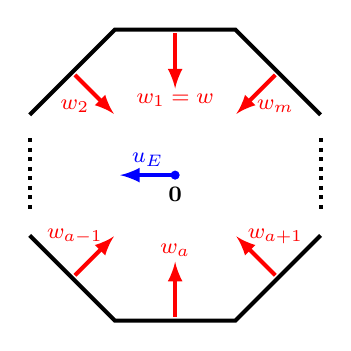
\begin{tikzpicture}[sarrow/.style={-latex, very thick}]
\foreach \name/\r in {0/2,1/2,2/2,3/2,4/2,5/2,6/2,7/2}{\coordinate (v\name) at (22.5+45*\name:\r cm);}
\draw [line width=0.05cm] (v0)--(v1)--(v2)--(v3); \draw [line width=0.05cm] (v4)--(v5)--(v6)--(v7);

\path (v3) ++(-90:0.3cm) coordinate (v3-); \path (v4) ++(90:0.3cm) coordinate (v4+);
\draw [line width=0.05cm, dotted] (v3-)--(v4+);
\path (v0) ++(-90:0.3cm) coordinate (v0-); \path (v7) ++(90:0.3cm) coordinate (v7+);
\draw [line width=0.05cm, dotted] (v0-)--(v7+);

\foreach \name in {1,2,3,5,6,7}{\coordinate (vec\name) at (45*\name:1.8 cm);}
\foreach \name in {1,2,3,5,6,7}{\draw[red, sarrow, line width=0.05cm] (vec\name)-- ++(180+45*\name:0.7cm);}

\path (vec1) ++(-90:0.4cm) node[red] {\footnotesize$w_m$};
\path (vec2) ++(-90:0.85cm) node[red] {\footnotesize$w_1=w$};
\path (vec3) ++(-90:0.4cm) node[red] {\footnotesize$w_2$};
\path (vec5) ++(90:0.5cm) node[red] {\footnotesize$w_{a-1}$};
\path (vec6) ++(90:0.85cm) node[red] {\footnotesize$w_a$};
\path (vec7) ++(90:0.5cm) node[red] {\footnotesize$w_{a+1}$};
\filldraw [blue] (0,0) circle [radius=0.05cm];
\draw[blue, sarrow, line width=0.05cm] (0,0)-- ++(180:0.7cm) node[inner sep=0.5pt, circle, midway, xshift=0cm, yshift=0.2cm, blue] {\footnotesize$u_E$};
\node at (0,-0.25) {\footnotesize${\bf 0}$};
\end{tikzpicture}
}
\caption{The PM polygon $\Delta_\Gamma$ and its inner normal vectors (the case where the origin is contained in the strict interior of $\Delta_\Gamma$).}
\label{PMpolygon_normalvec}
\end{figure}

First, we consider the edge $E_1$ and zigzag paths in $\calZ_{v_1}=\calZ_{(-w)}$.
By definition, we have $\langle -v_1,u_E\rangle=0$ and $\{z_1,\dots,z_r\}\subseteq\calZ_{(-w)}^\rmI\subseteq \calZ_{(-w)}$.
If $|\calZ_{(-w)}|>r$, then there exists a zigzag path in $\calZ_{(-w)}$ that is not in $\{z_1,\dots,z_r\}$.
If $E_a\neq\varnothing$, we have zigzag paths in $\calZ_{v_a}$.
Since $E_1$ and $E_a$ are parallel, $v_1$ and $v_a$ are linearly dependent, and hence $\langle v_a,u_E\rangle=0$.
Then, we see that zigzag paths in $\calZ_{v_a}$ do not intersect with any type I zigzag path $z$ satisfying $[z]=v_1$ in the universal cover (see Lemma~\ref{slope_linearly_independent}).

Next, we consider the edges $E_2,\dots,E_{a-1}$ of $\Delta_\Gamma$ and zigzag paths in $\calZ_1\coloneqq\calZ_{v_2}\cup\cdots\cup\calZ_{v_{a-1}}$.
We see that $v_i$ with $i=2,\dots,a-1$ satisfies $\langle -v_i,u_E\rangle<0$ by a choice of the edges $E_2,\dots,E_{a-1}$.
By the same argument as in the proof of Proposition~\ref{prop_nondegenerate}, we see that
the zigzag paths in $\calZ_1$ intersect with a type I zigzag path $z$ satisfying $[z]=v_1$ precisely once in the universal cover (see Lemma~\ref{slope_linearly_independent}); specifically, they intersect with $z$ in $\Zag(z)$.
Thus, we have $\calZ_1=\{x_1,\dots,x_s\}$, and for each $i=2,\dots ,a-1$ the vector $v_i$ satisfies $v_i=[x_j]$ for some $j=1,\dots,s$.

Next, we consider the edges $E_{a+1},\dots,E_m$ of $\Delta_\Gamma$ and zigzag paths in $\calZ_2\coloneqq\calZ_{v_{a+1}}\cup\cdots\allowbreak\cup\calZ_{v_m}$.
We see that~$v_i$ with $i=a+1,\dots,m$ satisfies $\langle -v_i,u_E\rangle>0$ by the choice of the edges $E_{a+1},\dots,E_m$.
By a similar argument as above, we see that the zigzag paths in $\calZ_2$ intersect with a type I zigzag path $z$ satisfying $[z]=v_1$ precisely once in the universal cover; specifically, they intersect with $z$ in $\Zig(z)$.
Thus, we have $\calZ_2=\{y_1,\dots,y_t\}$, and for each $i=a+1,\dots,m$ the vector $v_i$ satisfies $v_i=[y_k]$ for some $k=1,\dots,t$.

Collectively, we see that any zigzag path of $\Gamma$ takes one of the following forms:
\begin{itemize}\itemsep=0pt
\item $z_1,\dots,z_r$,
\item $z_1^\prime,\dots,z_{r^\prime}^\prime$ contained in $\calZ_{(-w)}{\setminus}\{z_1,\dots,z_r\}$ for $w=-v_1$ with $\langle w,u_E\rangle=0$ if $|\calZ_{(-w)}|>r$,
\item $z_1^{\prime\prime},\dots,z_{r^{\prime\prime}}^{\prime\prime}$ contained in $\calZ_w$ for $w=-v_1$ with $\langle w,u_E\rangle=0$ if $E_a\neq\varnothing$,
\item $x_j$ where $j=1,\dots,s$, in which case it satisfies $\langle-[x_j],u_E\rangle<0$,
\item $y_k$ where $k=1,\dots,t$, in which case it satisfies $\langle-[y_k],u_E\rangle>0$.
\end{itemize}
The slopes of these zigzag paths give the supporting hyperplanes of $\Delta_\Gamma$ by Proposition~\ref{zigzag_sidepolygon}. More precisely, if $\Delta_\Gamma$ contains the origin ${\bf 0}$ as an interior lattice point, then
\begin{displaymath}
H_{-[\zeta],\ge -k_\zeta}=\{u\in N_\RR\,|\,\langle-[\zeta],u\rangle\ge -k_\zeta\}
\end{displaymath}
is the supporting hyperplane of $\Delta_\Gamma$ for any zigzag path $\zeta$ of $\Gamma$ and a certain positive integer $k_\zeta$.
If the origin ${\bf 0}$ lies on the boundary of $\Delta_\Gamma$, $k_\zeta$ is replaced by $0$ for the zigzag paths corresponding to the edges that contain ${\bf 0}$.
By Proposition~\ref{prop_dual_polytope} and its proof, $\Delta_\Gamma^*$ can be written as $\Delta_\Gamma^*=Q+C$, where $Q$ is a polygon and $C$ is a polyhedral cone.
Since the set of the slopes of zigzag paths of $\Gamma$ coincides with $\{v_1,\dots,v_m\}$ if we identify the same slopes,
we see that the set $\{u_1,\dots,u_p,u_1^\prime,\dots,u_q^\prime\}$, which generates $Q$ and $C$ in the proof of Proposition~\ref{prop_dual_polytope},
is given by $\{w_1,\dots,w_m\}$ in our situation.
In what follows, we assume that ${\bf 0}$ is contained in the strict interior of $\Delta_\Gamma$, in which case $\Delta_\Gamma^*=Q$ and
$Q=\operatorname{conv}\big(\big\{\frac{1}{k_1}w_1,\dots,\frac{1}{k_m}w_m\big\}\big)$ for some positive integers $k_i$,
giving the supporting hyperplanes $H_{w_i,\ge-k_i}$ of $\Delta_\Gamma$ for $i=1,\dots,m$.
We remark that $\frac{1}{k_a}w_a$ appears in the above generating set if $E_a\neq\varnothing$.
Since $\langle w_i,u_E\rangle\ge0$ for $i=1,a, a+1,\dots, m$ and $\langle w_i,u_E\rangle<0$ for $i=2,\dots, a-1$,
we see that
\begin{gather}
\varphi(\Delta_\Gamma^*)=\operatorname{conv}\bigg(\bigg\{\frac{1}{k_1}w_1,\frac{1}{k_2}w_2^\prime,\dots,\frac{1}{k_{a-1}}w_{a-1}^\prime,
\frac{1}{k_a}w_a \ \text{(if $E_a\neq\varnothing$)}, \nonumber\\
\hphantom{\varphi(\Delta_\Gamma^*)=\operatorname{conv}\bigg(\bigg\{}{}
\frac{1}{k_{a+1}}w_{a+1}, \dots,\frac{1}{k_m}w_m\bigg\}\bigg),\label{generating_set_dual}
\end{gather}
where $w_i^\prime\coloneqq w_i-\langle w_i,u_E\rangle w$ for $i=2,\dots,a-1$.
We also note that when $E_a=\varnothing$, we can take the positive integer $k_a$ so that the line $\{u\in N_\RR\,|\,\langle v_1,u\rangle= -k_a\}$, which is parallel to $E_1$, passes through the vertex of $\Delta_\Gamma$ that is the intersection of $E_{a-1}$ and $E_{a+1}$.
By the choice of $k_a$, we have $\langle \frac{1}{k_a}v_1,u\rangle\ge -1$ for any $u\in \Delta_\Gamma$; thus $\frac{1}{k_a}v_1=\frac{1}{k_a}(-w_1)\in\Delta_\Gamma^*$ and hence $\frac{1}{k_a}v_1=\frac{1}{k_a}(-w_1)\in\varphi(\Delta_\Gamma^*)$.

We then consider the deformed dimer model $\nu^\zig_\calX(\Gamma)=\nu^\zig_\calX(\Gamma,\{z_1,\dots,z_r\})$.
By Observation~\ref{obs_deformed_part}, the lift of any zigzag path of the form $z_i^\prime$ or $z_i^{\prime\prime}$ on the universal cover is contained in some irrelevant part, and hence it does not change even if we apply the extended deformation.
Also, by Proposition~\ref{zigzag_afterdeform2}, we have the zigzag paths $x_1^\prime,\dots,x_s^\prime$ on $\nu^\zig_\calX(\Gamma)$ satisfying
\begin{displaymath}
-[x^{\prime}_j]=-[x_j]-\langle [x_j],h(\sfP_z^\prime,\sfP_z)\rangle[z]=w_i-\langle w_i,u_E\rangle w
\end{displaymath}
for $j=1,\dots,s$ and some $i=2,\dots,a-1$.
Furthermore, by Proposition~\ref{zigzag_afterdeform1}, we have the zigzag paths $y_1^\prime,\dots,y_t^\prime$ on $\nu^\zig_\calX(\Gamma)$ satisfying
\begin{displaymath}
-[y_k^\prime]=-[y_k]=w_i
\end{displaymath}
for $k=1,\dots,t$ and some $i=a+1,\dots,m$.
Thus, we see that the zigzag paths $x_j, y_k$ vary as they satisfy the condition (\ref{mutation_M}) when we apply the extended deformation $\nu^\zig_\calX$ to $\Gamma$.
In addition, we have the zigzag path of the form $z_{i,j}$ defined in (zig-3).
Thus, the zigzag paths on the consistent dimer model $\nu^\zig_\calX(\Gamma)$ are
\begin{gather*}
\{z_i^\prime\}_{1\le i\le r^\prime}\quad \text{(if $|\calZ_{(-w)}|>r$)},\qquad \{z_i^{\prime\prime}\}_{1\le i\le r^{\prime\prime}}\quad \text{(if $E_a\neq\varnothing$)},\\
\{x_j^\prime\}_{1\le j\le s},\qquad \{y_k^\prime\}_{1\le k\le t},\qquad \text{and} \qquad \{z_{i,j}\}_{\substack{1\le i\le r \\ 1\le j\le p_i}}.
\end{gather*}
By the description of their slopes and Proposition~\ref{zigzag_sidepolygon}, we see that the inner normal vectors of~$\Delta_{\nu^\zig_\calX(\Gamma)}$ are
\begin{displaymath}
\{w_1,w_2^\prime,\dots,w_{a-1}^\prime,w_a=-w_1, w_{a+1}, \dots,w_m\},
\end{displaymath}
and these vectors give the supporting hyperplanes of $\Delta_{\nu^\zig_\calX(\Gamma)}$ just like for $\Delta_\Gamma$.
Here, $w_1$ appears in the above set if $|\calZ_{(-w_1)}|=|\calZ_{v_1}|>r$,
but we always have $\frac{1}{k_1}w_1\in \Delta_{\nu^\zig_\calX(\Gamma)}^*$ by the same argument as we used for showing $\frac{1}{k_a}(-w_1)\in\Delta_\Gamma^*$ above, whereas $w_a$ certainly appears since $[z_{i,j}]=-[z_i]=-w_1=w_a$ (see Lemma~\ref{deform_vector}). Thus, we have
\begin{displaymath}
\Delta_{\nu^\zig_\calX(\Gamma)}^*=\operatorname{conv}\bigg(\bigg\{\frac{1}{k_1}w_1,\frac{1}{k_2}w_2^\prime,\dots,\frac{1}{k_{a-1}}w_{a-1}^\prime,
\frac{1}{k_a}w_a, \frac{1}{k_{a+1}}w_{a+1}, \dots,\frac{1}{k_m}w_m\bigg\}\bigg).
\end{displaymath}
By the description (\ref{generating_set_dual}) and the fact that $\frac{1}{k_1}w_1$ and $\frac{1}{k_a}w_a=\frac{1}{k_a}(-w_1)$ are contained in both $\varphi(\Delta_\Gamma^*)$ and $\Delta_{\nu^\zig_\calX(\Gamma)}^*$, we see that $\varphi(\Delta_\Gamma^*)=\Delta_{\nu^\zig_\calX(\Gamma)}^*$.

The case where the origin ${\bf 0}$ lies on the boundary of $\Delta_\Gamma$ can be proved by a similar argument if we consider the hyperplane $\{u\in N_\RR\,|\,\langle-[\zeta],u\rangle\ge 0\}$ instead of $\{u\in N_\RR\,|\,\langle-[\zeta],u\rangle\ge -k_\zeta\}$ for the zigzag paths corresponding to the edges that contain ${\bf 0}$, in which case $-[\zeta]$ will be a~generator of a polyhedral cone~$C$.

By Propositions~\ref{prop_dual_polytope}(ii) and \ref{prop_mutation_dual_polytope}, we conclude that
$\mutation_{w}(\Delta_\Gamma,F)=\Delta_{\nu^\zig_\calX(\Gamma)}$.
\end{proof}
\begin{thebibliography}{99}
\bibitem[2]{ACGK}
Akhtar M., Coates T., Galkin S., Kasprzyk A.M., Minkowski polynomials and
 mutations, \href{https://doi.org/10.3842/SIGMA.2012.094}{\textit{SIGMA}} \textbf{8} (2012), 094, 707~pages,
 \href{https://arxiv.org/abs/1212.1785}{arXiv:1212.1785}.

\bibitem[3]{BIU}
Beil C., Ishii A., Ueda K., Cancellativization of dimer models,
 \href{https://arxiv.org/abs/1301.5410}{arXiv:1301.5410}.

\bibitem[4]{Boc1}
Bocklandt R., Consistency conditions for dimer models, \href{https://doi.org/10.1017/S0017089512000080}{\textit{Glasg. Math.~J.}}
 \textbf{54} (2012), 429--447, \href{https://arxiv.org/abs/1104.1592}{arXiv:1104.1592}.

\bibitem[7]{Bro}
Broomhead N., Dimer models and {C}alabi--{Y}au algebras, \href{https://doi.org/10.1090/S0065-9266-2011-00617-9}{\textit{Mem. Amer.
 Math. Soc.}} \textbf{215} (2012), viii+86~pages, \href{https://arxiv.org/abs/0901.4662}{arXiv:0901.4662}.

\bibitem[10]{Duf}
Duffin R.J., Potential theory on a rhombic lattice, \href{https://doi.org/10.1016/S0021-9800(68)80072-9}{\textit{J.~Combinatorial
 Theory}} \textbf{5} (1968), 258--272.

\bibitem[11]{FHK}
Franco S., Hanany A., Vegh D., Wecht B., Kennaway K.D., Brane dimers and quiver
 gauge theories, \href{https://doi.org/10.1088/1126-6708/2006/01/096}{\textit{J.~High Energy Phys.}} \textbf{2006} (2006), no.~1,
 096, 48~pages, \href{https://arxiv.org/abs/hep-th/0504110}{arXiv:hep-th/0504110}.

\bibitem[14]{Gul}
Gulotta D.R., Properly ordered dimers, {$R$}-charges, and an efficient inverse
 algorithm, \href{https://doi.org/10.1088/1126-6708/2008/10/014}{\textit{J.~High Energy Phys.}} \textbf{2008} (2008), no.~10, 014,
 31~pages, \href{https://arxiv.org/abs/0807.3012}{arXiv:0807.3012}.

\bibitem[16]{HV}
Hanany A., Vegh D., Quivers, tilings, branes and rhombi, \href{https://doi.org/10.1088/1126-6708/2007/10/029}{\textit{J.~High Energy
 Phys.}} \textbf{2007} (2007), no.~10, 029, 35~pages, \href{https://arxiv.org/abs/hep-th/0511063}{arXiv:hep-th/0511063}.

\bibitem[19]{IU1}
Ishii A., Ueda K., A note on consistency conditions on dimer models, in Higher
 Dimensional Algebraic Geometry, \textit{RIMS K\^oky\^uroku Bessatsu}, Vol.~B24, Res. Inst. Math. Sci. (RIMS), Kyoto, 2011, 143--164, \href{https://arxiv.org/abs/1012.5449}{arXiv:1012.5449}.

\bibitem[20]{IU2}
Ishii A., Ueda K., Dimer models and the special {M}c{K}ay correspondence,
 \href{https://doi.org/10.2140/gt.2015.19.3405}{\textit{Geom. Topol.}} \textbf{19} (2015), 3405--3466, \href{https://arxiv.org/abs/0905.0059}{arXiv:0905.0059}.

\bibitem[22]{KNP}
Kasprzyk A., Nill B., Prince T., Minimality and mutation-equivalence of
 polygons, \href{https://doi.org/10.1017/fms.2017.10}{\textit{Forum Math. Sigma}} \textbf{5} (2017), e18, 48~pages,
 \href{https://arxiv.org/abs/1501.05335}{arXiv:1501.05335}.

\bibitem[25]{KS}
Kenyon R., Schlenker J.M., Rhombic embeddings of planar quad-graphs,
 \href{https://doi.org/10.1090/S0002-9947-04-03545-7}{\textit{Trans. Amer. Math. Soc.}} \textbf{357} (2005), 3443--3458,
 \href{https://arxiv.org/abs/math-ph/0305057}{arXiv:math-ph/0305057}.

\bibitem[26]{Mer}
Mercat C., Discrete {R}iemann surfaces and the {I}sing model, \href{https://doi.org/10.1007/s002200000348}{\textit{Comm.
 Math. Phys.}} \textbf{218} (2001), 177--216, \href{https://arxiv.org/abs/0909.3600}{arXiv:0909.3600}.

\bibitem[30]{Sch}
Schrijver A., Theory of linear and integer programming, \textit{Wiley-Interscience
 Series in Discrete Mathematics}, John Wiley \& Sons, Ltd., Chichester, 1986.

\end{thebibliography}
\end{document}
